\chapter{CLIC Experimental Conditions and Detector Requirements\label{chapter_03}}

%%----------------------------------------------------------------------------------------------------------------------

In this chapter the design requirements for a detector at CLIC are described.
These requirements are driven both by the physics at CLIC, potentially operating
over a range of centre-of-mass energies, and by the machine environment and
related backgrounds at the interaction point (IP). 

%%----------------------------------------------------------------------------------------------------------------------

\section{The CLIC Experimental Environment\label{sec:chapter3:environment}}

The main parameters of the CLIC beam of relevance to the physics reach of the
machine and the related levels of background at the \acs{IP} are summarised in
Table~\ref{tab:chap3:clicBeam} (see also~\cite{CLICacceleratorCDR}).
\begin{table}[!hbt]
  \centering
  \begin{threeparttable}
  \captionsetup{width=\linewidth}
  \caption{The main parameters of the CLIC machine and background rates at the interaction point.
    The listed variables are:
    $\theta_c$ the horizontal crossing angle of the beams at the IP;
    $f_{\mathrm{rep}}$, the repetition frequency;
    $n_\mathrm{b}$, the number of bunches per bunch train;
    $\Delta t$, the separation between bunches in a train;
    $N$, the number of particles per bunch;
    $\sigma_\mathrm{x}$, $\sigma_\mathrm{y}$, and $\sigma_\mathrm{z}$, the bunch dimensions at the \acs{IP};
    % the normalised horizontal/vertical emittance at the IP, $\epsilon_x$ and $\epsilon_y$ ;
    $\beta_x$ and $\beta_y$ the beta functions at the IP;
    \acs{L$^*$} the distance from the last quadrupole to the IP;
    ${\cal{L}}$, the design luminosity;
    ${\cal{L}}_{0.01}$, the luminosity with $\rootsprime>0.99\roots$;
    $\Delta E/E$, the average fraction loss of energy from beamstrahlung;
    $n_\upgamma$, the average number of beamstrahlung photons per beam
    particle;
    $N_{\mathrm{coh}}$, the number of coherent pair particles per
    bunch crossing (BX);
    $E_{\mathrm{coh}}$, the total energy of coherent pair particles per BX;
    $N_{\mathrm{incoh}}$, the number of incoherent pair particles per BX;
    $E_{\mathrm{incoh}}$, the total energy of incoherent pair particles per BX;
    and,  $n_{\mathrm{Had}}$, the number of \gghadrons events per BX
    for a threshold of 2~GeV.  %%$\sqrt{s_{\gamma\gamma}}>5$~GeV,
                               %%$n_{\mathrm{Had}}$. 
    The backgrounds rates and energy releases are quoted excluding
    safety factors for the simulation uncertainties.
    \label{tab:chap3:clicBeam}}
  \begin{tabular}{c c c c}
    \toprule
    Parameter              & Units               & $\roots=500$~GeV   & $\roots=3$~TeV     \\  \midrule
    $\theta_c$    &      mrad&       18.6   &        20          \\
    $f_{\mathrm{rep}}$     & Hz                  & 50                 & 50                 \\
    $n_{\mathrm{b}}$       &                     & 354                & 312                \\
    $\Delta t$             & ns                  & 0.5                & 0.5                \\
    $N$                    &                     & $6.8 \cdot 10^9$    & $3.72 \cdot 10^9$    \\
    $\sigma_x$             & nm                  & 202                & $\approx 45$        \\
    $\sigma_y$             & nm                  & 2.26               & $\approx 1$         \\
    $\sigma_z$             & \micron             & 72                 & 44                 \\
    %% $\epsilon_x$        & $\upmu$m            & 2.4                & 0.66               \\
    %% $\epsilon_y$        & nm                  & 25                 & 20                 \\
    $\beta_x$           & mm                  & 8                  & 4                  \\
    $\beta_y$           & mm                  & 0.1                & 0.07               \\  
    {L$^*$}~\tnote{a}   &     m            &  3.5                &  3.5         \\
    %%\acs{L$^*$} (\clicild)            &     m       &              4.3               &       4.3         \\
    %%\midrule
    ${\cal{L}}$            & $\rm cm^{-2}s^{-1}$ & $2.3 \cdot 10^{34}$ & $5.9 \cdot 10^{34}$ \\
    ${\cal{L}}_{0.01}$     & $\rm cm^{-2}s^{-1}$ & $1.4 \cdot 10^{34}$ & $2.0 \cdot 10^{34}$ \\
    $n_\upgamma$           &                     & 1.3                & 2.1                \\
    {$\Delta E/E$}         &                     & {$0.07$}           & {$0.28$}           \\ \midrule
    {$N_{\mathrm{coh}}$}   &                     & {$2 \cdot 10^{2}$}  & {$6.8 \cdot 10^8$}  \\
    {$E_{\mathrm{coh}}$}   & TeV                 & {$1.5 \cdot 10^1$}  & {$2.1 \cdot 10^8$}  \\ \midrule
    {$N_{\mathrm{incoh}}$} &                     & {8$ \cdot 10^4$}    & {3$ \cdot 10^5$}    \\
    {$E_{\mathrm{incoh}}$} & TeV                 & 3.6$ \cdot 10^2$    & 2.3$ \cdot 10^4$    \\ \midrule
    {$n_{\mathrm{Had}}$} ($W_{\upgamma\upgamma}>$2~GeV)   &                     & {0.3}             & {3.2}              \\\bottomrule
  \end{tabular}
\begin{tablenotes}
\item[a] This value holds for SiD, and has been used throughout the accelerator studies for this CDR\@. For ILD, the corresponding value is 4.3~m.
\end{tablenotes}
\end{threeparttable}
\end{table}

The experimental environment at CLIC differs from that at previous \epem
colliders such as \acs{LEP} and also the proposed \acs{ILC}. In particular, there are three
main aspects of the CLIC machine that determine the physics environment and
significantly impact the CLIC detector design:
\begin{itemize}
\item The high bunch charge density, related to the small beam size at the
interaction point, means that the electrons and positrons radiate strongly
in the electromagnetic field of the other beam, an effect known as
beamstrahlung (similar to synchrotron radiation). Consequently the 
centre-of-mass energies of the \epem collision have a long tail towards
significantly lower values than the notional centre-of-mass energy (discussed
in Section~\ref{sec:chapter3:environment:beam}). 
\item There are significant beam related backgrounds. The \epem incoherent
pair background has a major impact on the design of the inner region of the
detector and the forward region. The pile-up of approximately 3.2
\gghadrons ``mini-jet'' events per bunch crossing (BX) impacts the timing
requirements placed on the individual detector elements and is an important
consideration in all physics analyses (discussed in
Section~\ref{sec:chapter3:environment:beambackgrounds})
\item The CLIC beam consists of bunch trains of 312 bunches with a train
repetition rate of 50~Hz. Within a bunch train, the bunches are separated
by 0.5~ns. The short time between bunches means that a detector will
inevitably integrate over a number of bunch crossings. This combined with
the significant \gghadrons background implies fast readout of all detector
elements and excellent time resolution (discussed in
Section~\ref{sec:chapter3:clic_detector:timingRequirements}). 
\end{itemize} 

\subsection{The CLIC Beam \label{sec:chapter3:environment:beam}}

The intrinsic r.m.s. energy spread of CLIC beams is 0.35\%. In addition, due to
variations of the main linac accelerating \acs{RF} voltage and phase, the mean beam
energy is expected to be subject to a jitter of the order of 0.1\%. However, due
to beamstrahlung, not all the \epem collisions at CLIC will take place at the
nominal centre-of-mass energy. The impact of beamstrahlung on physics
measurements is not unlike that of initial state radiation (ISR); the colliding
electron and positron may radiate a high energy photon before the collision
and, consequently, the centre-of-mass energy of the electron-positron
collision \rootsprime is less than the nominal centre-of-mass energy of the
machine \roots. This results in an effective centre-of-mass spectrum (the
luminosity spectrum) with a peak at \roots corresponding to collisions with
no beamstrahlung and a long tail towards lower energies.
Figure~\ref{fig:chap3:lumiSpectrum} shows the luminosity spectrum for CLIC
operating at 500~GeV and 3~TeV. The long tail from beamstrahlung is
particularly evident at $\roots = 3~\mathrm{TeV}$; the effect of beamstrahlung is less
evident for the 500~GeV machine. 

\begin{figure}[hbt]
  \centering
  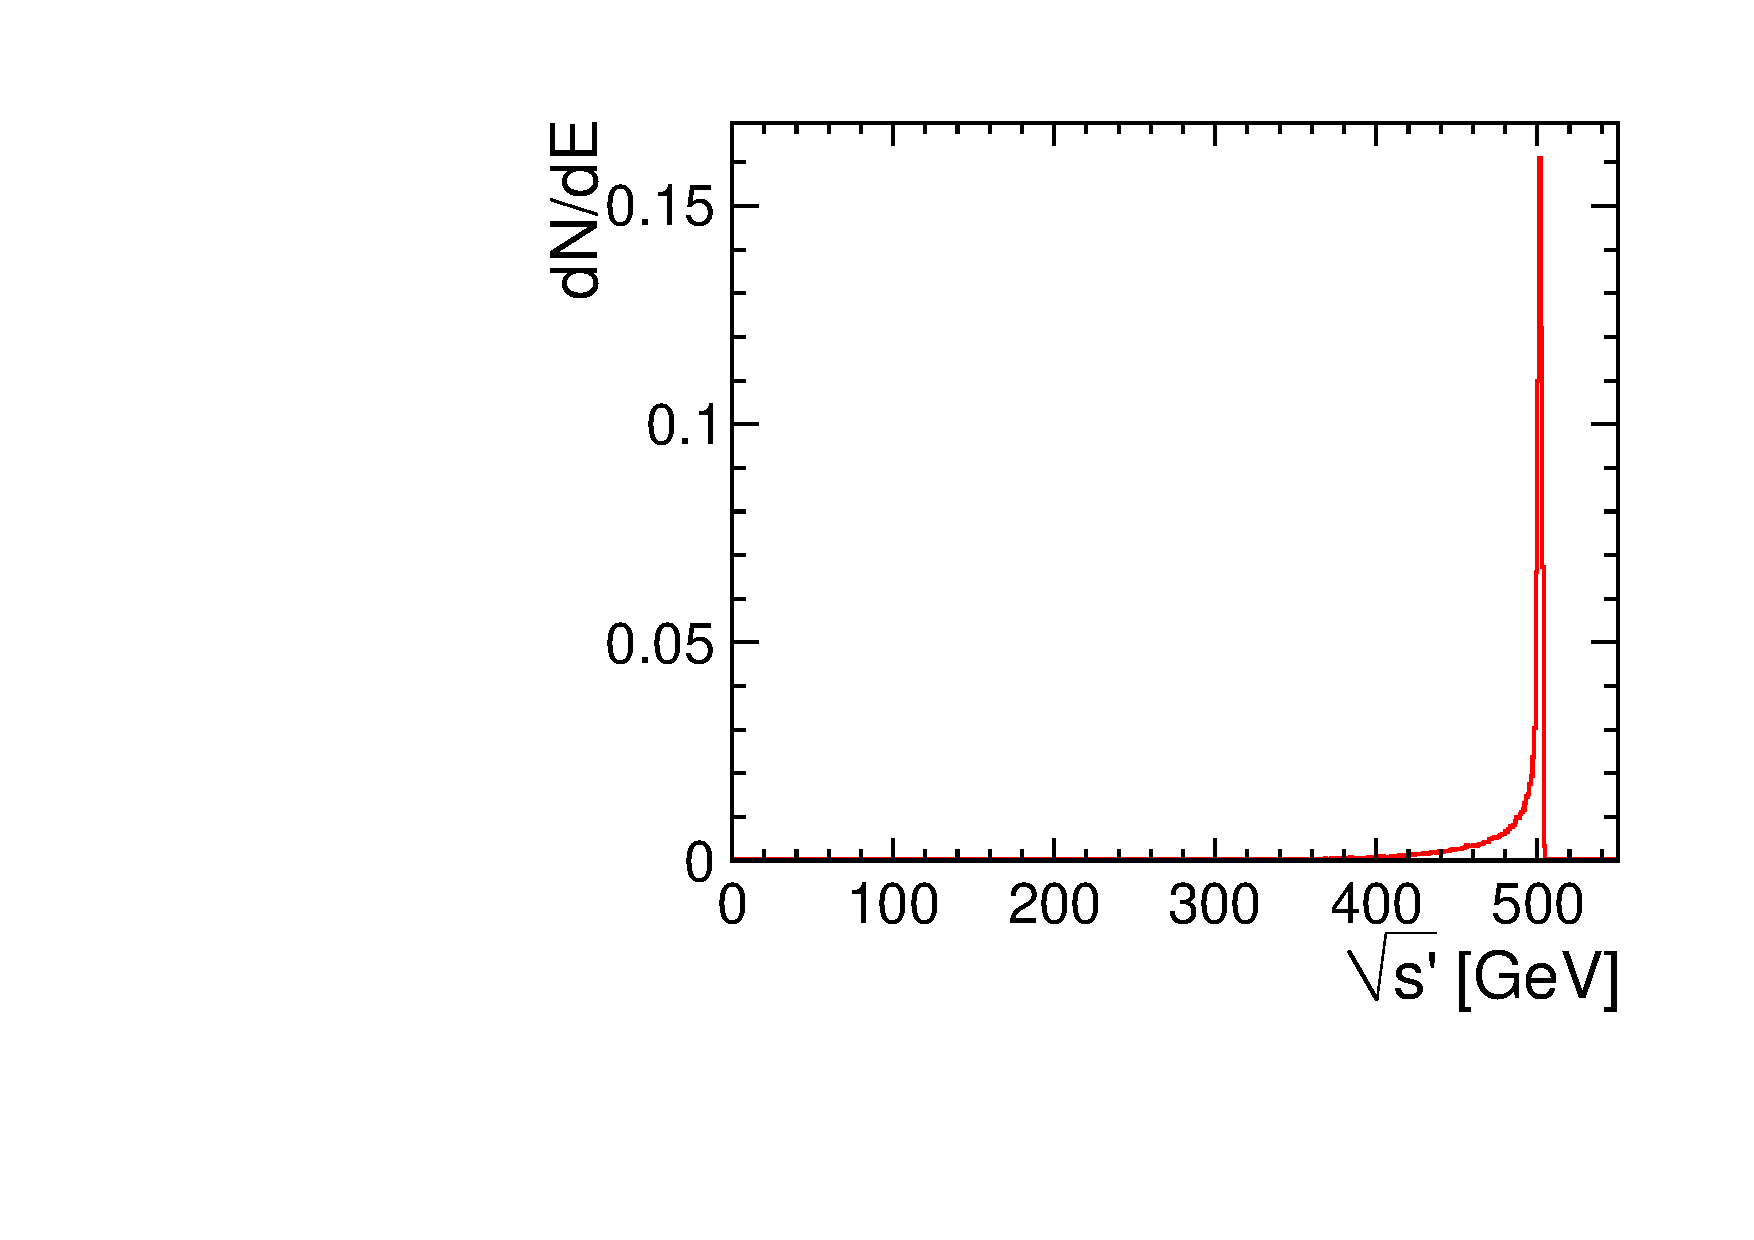
\includegraphics[width=0.49\linewidth]{../Chap3_ExpCond_PhysPerfsReqs/Lumi500GeV_fixed.pdf}
  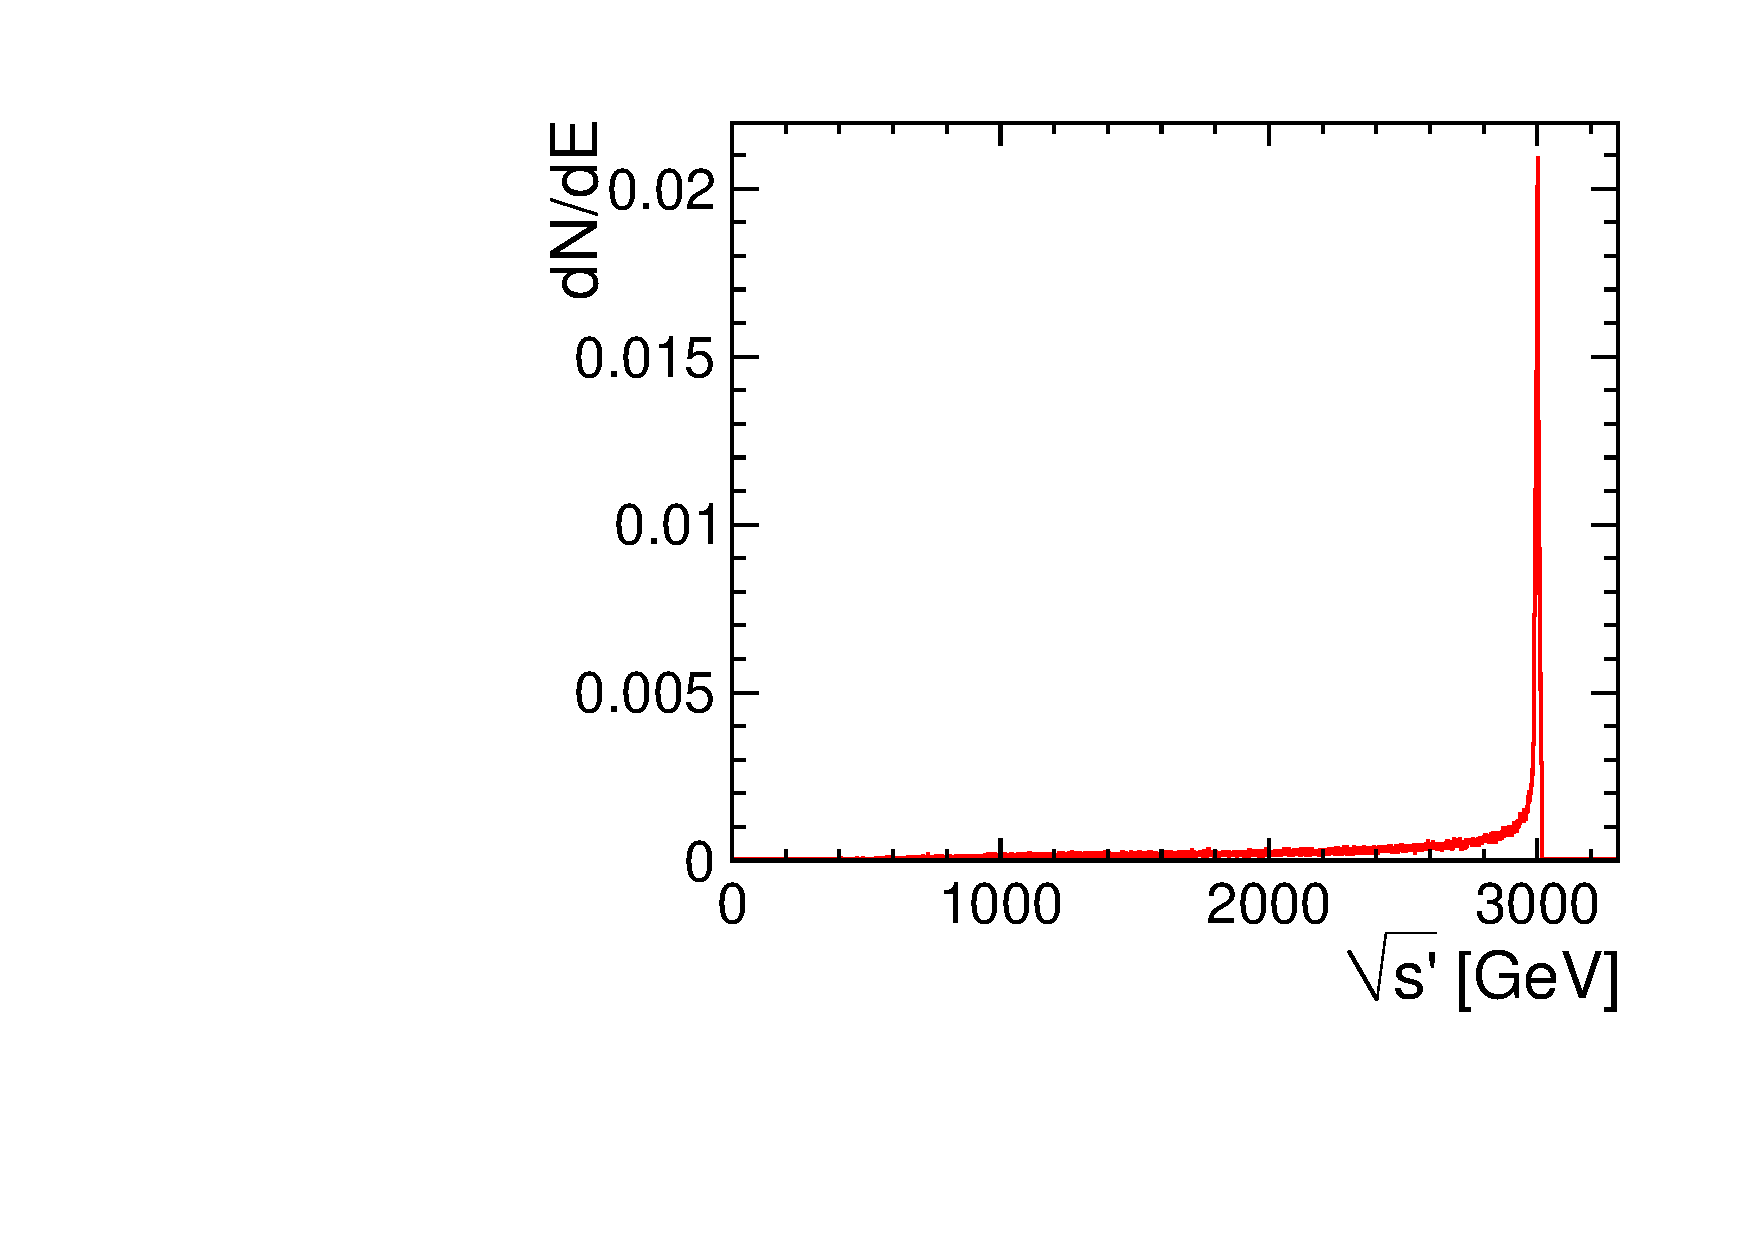
\includegraphics[width=0.49\linewidth]{../Chap3_ExpCond_PhysPerfsReqs/Lumi3TeV_fixed_nopeak.pdf}
  \caption{The luminosity spectrum for CLIC operating at (left)$\roots=500$~GeV and
    (right)$\roots=3$~TeV.\label{fig:chap3:lumiSpectrum}}
\end{figure}

The impact of the luminosity spectrum on the physics reach of CLIC is not simple
to quantify; it depends on the physics process being studied. At the most basic
level it reduces the amount of luminosity available at the highest
centre-of-mass energies. This is quantified in
Table~\ref{tab:chap3:lumiSpectrum}. For CLIC operating at 3~TeV only 35\% of
the effective luminosity is within 1\% of the nominal centre-of-mass energy.
However, this number should not be over-emphasised. Unless a \Zprime
is discovered, in which the production cross section is likely to be large,
physics at CLIC is unlikely to involve operation at the peak of a resonance.
Hence the useful luminosity will depend on the threshold of the process being
studied; for example, for CLIC operation at 3~TeV the useful luminosity for a
process with a threshold of 2~TeV is greater than 75\%. In addition to
reducing the effective useful luminosity, the effect of beamstrahlung has the
potential to distort the reconstructed particle energy spectrum in a number of
physics analyses (for example \acs{SUSY} decays involving the \acs{LSP}). This aspect is
discussed below and later in Chapter~\ref{chapter_14}.

\subsection{Beam-Induced Backgrounds\label{sec:chapter3:environment:beambackgrounds}}

There are three main sources of beam related backgrounds at CLIC:
\begin{itemize}
 \item \epem pairs which are predominantly produced with low transverse momenta \pT;
 \item \gghadrons which result in pile-up of low energy particles with $\pT \lesssim 5~\mathrm{GeV}$;
 \item beam halo muons.
\end{itemize}
Each background has been studied in detail and the impact on the detector
design has been carefully evaluated using full \geant simulations of the CLIC
detector concepts which are described in Section~\ref{sec:chapter3:detector_requirements} and
Chapter~\ref{chapter_05}. The beam-beam
backgrounds are estimated from simulation. First, the particles in the CLIC beams are
tracked from the beginning of the main linac to the interaction
point~\cite{Schulte:572820}. Then the resulting distributions are used,
without modifications or approximations,
as input for the beam-beam simulation code
\guineapig~\cite{Schulte:1999tx} which uses the known cross sections for the
relevant physical processes~\cite{Schulte1996}. 
Uncertainties on the simulation of the production rates and of the
detector response have been estimated. As a result, safety factors of
two for the background rates from \gghadrons and five for the ones
from \epem pairs have been estimated. Details are described
elsewhere~\cite{barklow_bg,lcd:2011-DannheimSailerBgrNote}.
Throughout this document,
results obtained with nominal parameters are presented in most tables
and figures, while safety factors are mentioned explicitly in the text.

\begin{table}[h]
  \centering
  \caption{\label{tab:chap3:lumiSpectrum} Fraction of luminosity above $\rootsprime/\roots$.}
  \begin{tabular}{c  *2{c}} \toprule
    \tabt{Fraction \rootsprime/\roots} & \tabt{500~GeV} & \tabt{3~TeV} \\ \midrule
    $>0.99$                            & 62\%           & 35\%         \\
    $>0.90$                            & 89\%           & 54\%         \\
    $>0.80$                            & 97\%           & 68\%         \\
    $>0.70$                            & 99.3\%         & 76\%         \\
    $>0.50$                            & 99.9\%         & 88\%         \\\bottomrule
  \end{tabular}
\end{table}


\subsubsection{Pair Background\label{sec:chapter3:environment:pairs}}

The large flux of beamstrahlung photons will produce \epem pairs in the strong
electromagnetic fields of the electron and positron bunches, both by coherent
and incoherent pair creation processes~\cite{Chen:242895}. The coherent
process consists of the interaction of the real beamstrahlung photons with the
collective electromagnetic field of the opposite beam. The coherent production
of \epem pairs will increase the total number of colliding electrons and
positrons by about 9\%. The production of coherent pairs from the virtual
photons associated with the beam particles (trident pairs) is roughly an order
of magnitude lower than the production of coherent pairs~\cite{c:jakob}. The
incoherent production of pairs arises from the interaction of both real or
virtual photons with \textit{individual} particles of the other beam. There are
three main physical processes responsible for the production of incoherent
pairs: the Breit-Wheeler (BW) process which is the interaction between two real
photons from beamstrahlung; the Bethe-Heitler (BH) process of the interaction
of a real photon and a virtual photon associated with a beam particle; and the
Landau-Lifshitz (LL) process of the interaction between two virtual photons. The
\guineapig calculation for the BH and LL processes uses a
Weizs\"{a}cker-Williams approach, known as the Equivalent Photon Approximation
(EPA). In the EPA, the equivalent spectrum of virtual photons is convolved
with the real photon interaction cross sections. The production of incoherent
pairs in \guineapig has been compared to other codes in~\cite{Schulte1996}
and~\cite{Rimbault:2005td}.


Most pairs are produced with very small angles along the beam axis. In order to
avoid significant loss of such particles in the detector, a beam exit line with
a half-cone opening angle of 10~mrad is needed, see
Figure~\ref{fig4.5}.
However, depending on the motion of the produced electron and positron with
respect to the electron and positron beams they may either be focused or
defocused. The effect of this electromagnetic beam deflection gives rise to
a component of the pair spectrum with sufficient transverse momentum for it to
travel beyond the beam pipe, and thus represent a potential background in the
detector volume. The effect of beam deflection on the coherent pairs is
relatively small as they are typically very high energy particles which are
highly boosted along the beam direction. Consequently, whilst the coherent pair
rate is extremely high, $7\cdot 10^8$ particles per bunch crossing at
3~TeV, almost all of the coherent pairs are collinear with the outgoing beams
and thus do not constitute a major detector background. 

While the number of incoherent pairs is much smaller than that of the coherent
pairs (see Table~\ref{tab:chap3:clicBeam}), they can be produced at larger
angles and potentially provide a significant source of background hits, for example, in
the inner layers of the vertex detector. The energy and angular distributions of
the pair backgrounds are shown in Figure~\ref{fig:chap3:background}. Because of
their larger transverse momentum, the incoherent pairs cause more energy
deposits in the detector and are a more relevant background source than the
coherent pairs, despite the much larger number of coherent pairs.

\begin{figure}[hbt]
\centering
 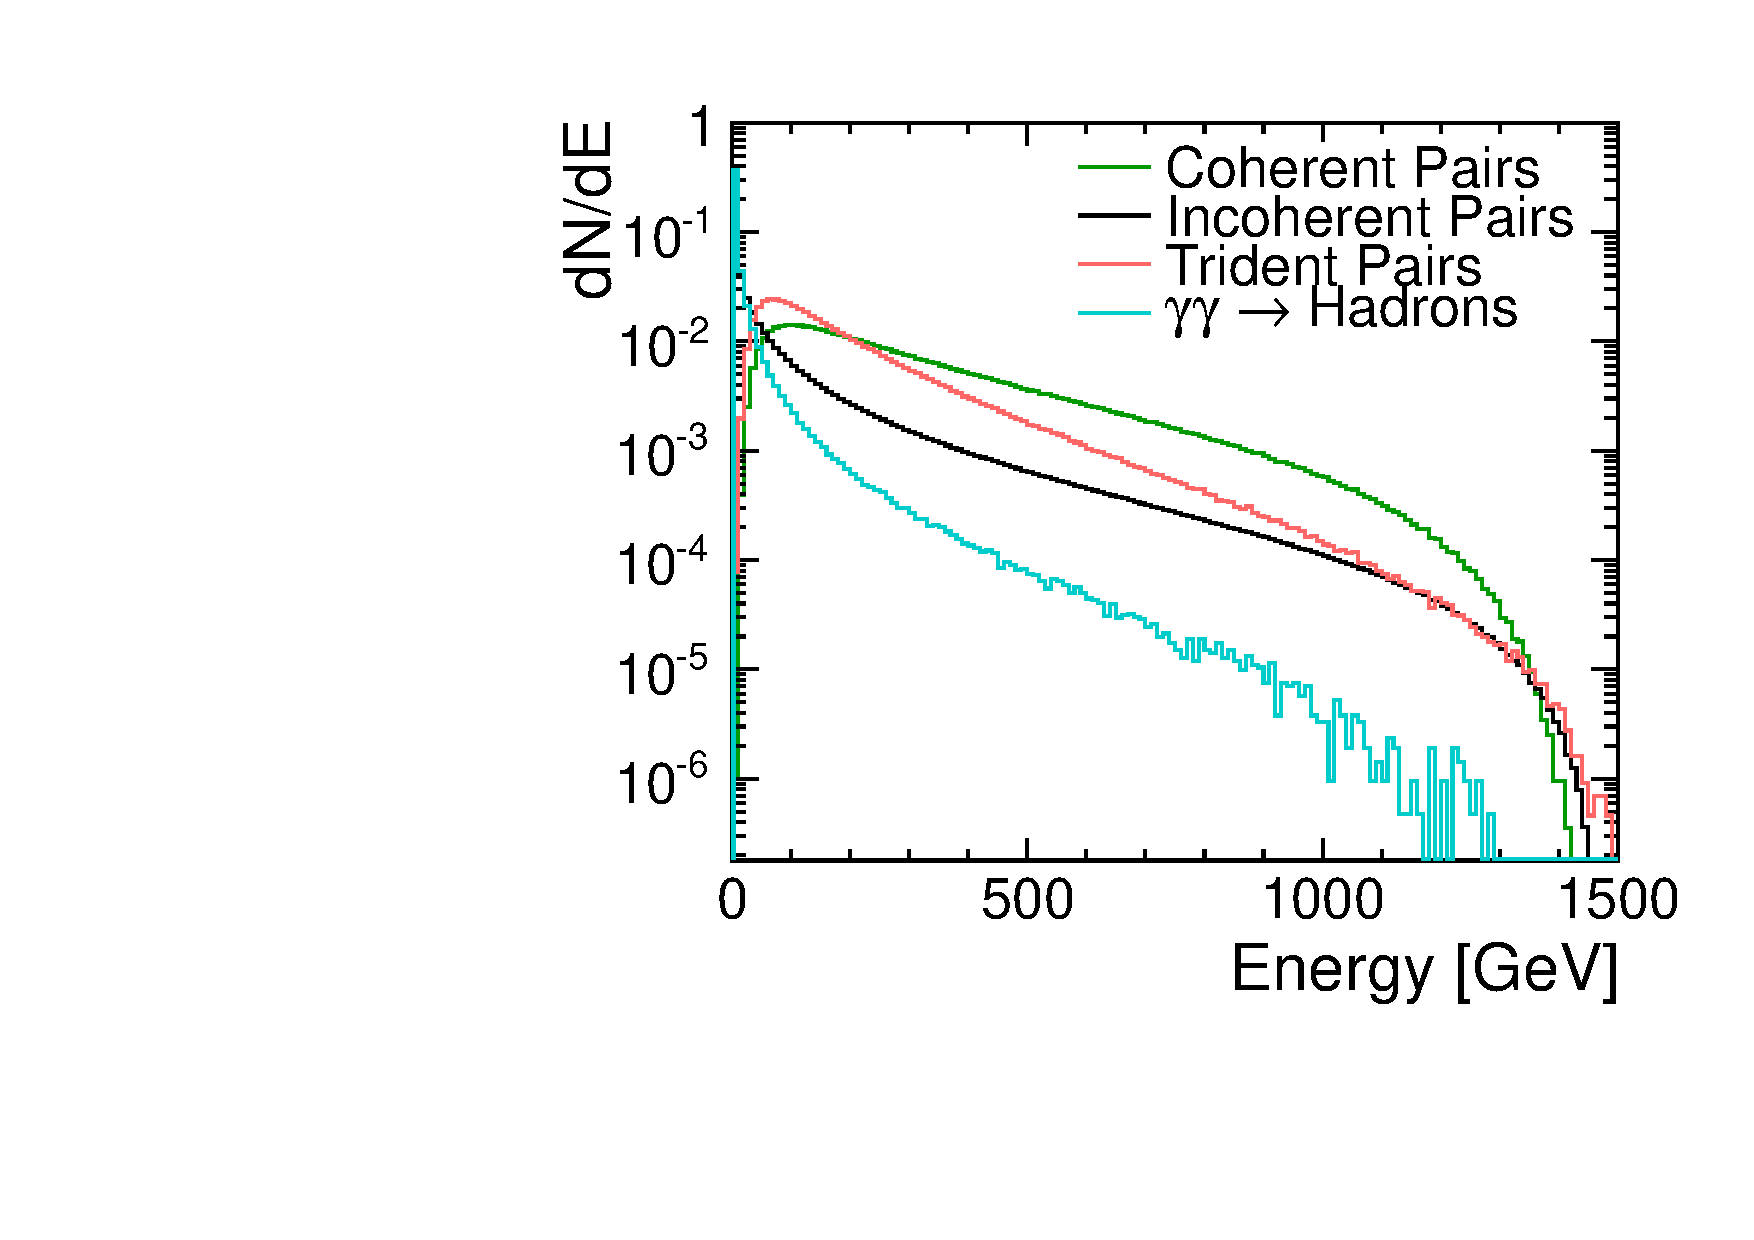
\includegraphics[width=0.49\linewidth]{../Chap3_ExpCond_PhysPerfsReqs/Energy.pdf} 
 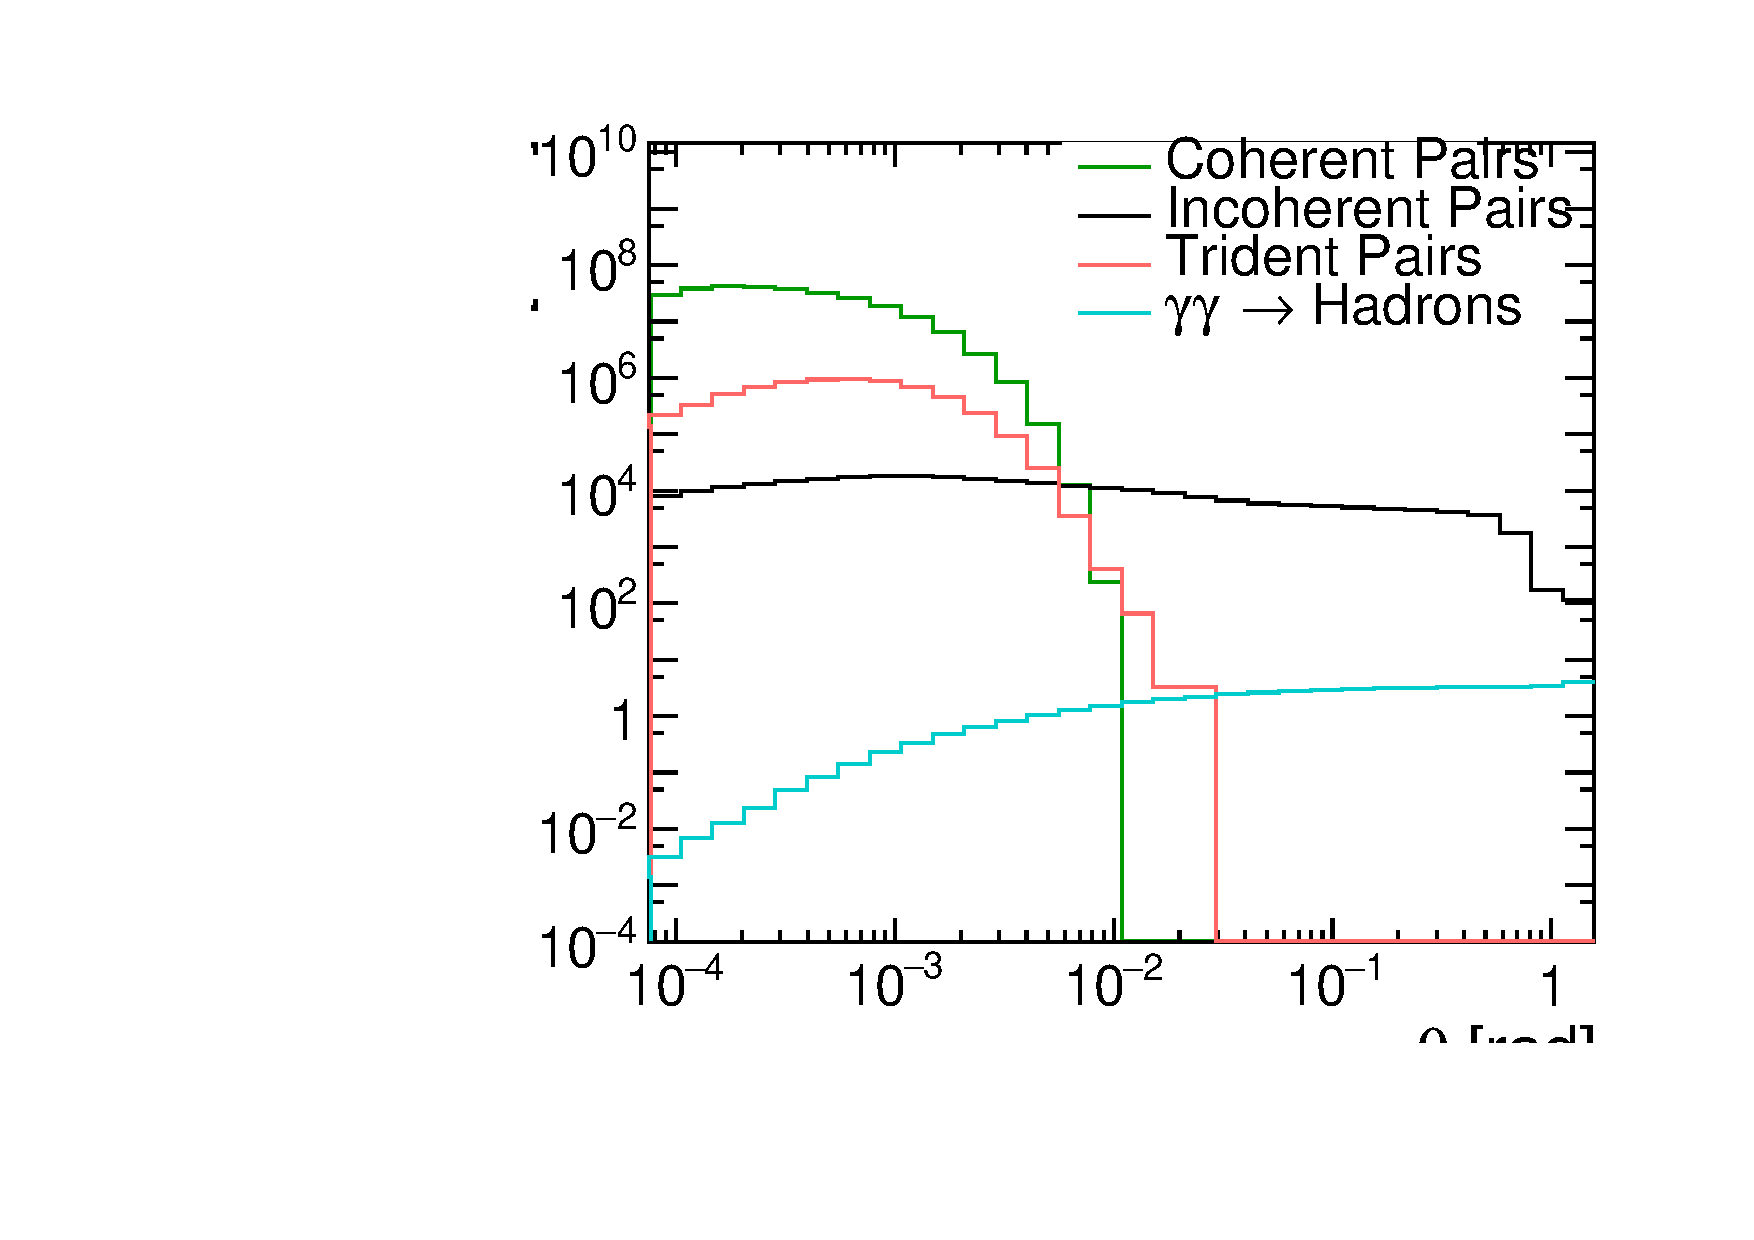
\includegraphics[width=0.49\linewidth]{../Chap3_ExpCond_PhysPerfsReqs/Angle.pdf}
 \caption{The distributions of the beam related backgrounds: (left) Fraction of
   energies for the particles of each background source. (right)
   Angular distribution of the produced background particles. Both plots are for
   CLIC at $\roots=3~\mathrm{TeV}$.\label{fig:chap3:background}}
\end{figure}


\subsubsection{Two-photon Background\label{sec:chapter3:environment:gammagamma}}

The interaction of real and virtual photons from the colliding beams can also
lead to multi-peripheral two-photon interactions producing hadronic final
states~\cite{dreesgodbole1991,Chen:561345}. The energy and
angular distributions of \gghadrons backgrounds are shown in
Figure~\ref{fig:chap3:background}. These interactions can produce particles at
a large angle to the beam line and constitute the main background for the
central tracking volumes and the calorimeters. 
The simulation of \gghadrons uses the photon spectrum from \guineapig and
a parametrisation of the total cross section based on~\cite{Schuler:1996en}: 
\begin{equation}
\sigma_{\gamgam}(s_{\gamgam})= 211~\mathrm{nb}\left(\frac{s_{\gamgam}}{\mathrm{GeV}^2}\right)^{0.0808} +215~\mathrm{nb}\left(\frac{s_{\gamgam}}{\mathrm{GeV}^2}\right)^{-0.4525}
\end{equation}
The predicted number of \gghadrons events per bunch crossing within the
detector acceptance at $\roots=3~\mathrm{TeV}$ is 3.2 for a \gamgam centre-of-mass
energy greater than 2~GeV. For a \gamgam centre-of-mass energy greater than
5~GeV, 2.8 \gghadrons events per bunch crossing are expected~\cite{barklow_bg}.

For the purpose of evaluating the impact of the \gghadrons background in the
detector, the spectrum of colliding photons from \guineapig are used to
generate events using the \pythia program~\cite{Sjostrand2006} which
simulates the hard interaction and the subsequent hadronisation. The resulting
\pT distribution of the produced particles which are within the detector acceptance is shown
in Figure~\ref{fig:chap3:gghad-pt}.

\begin{figure}[hbt]
\centering
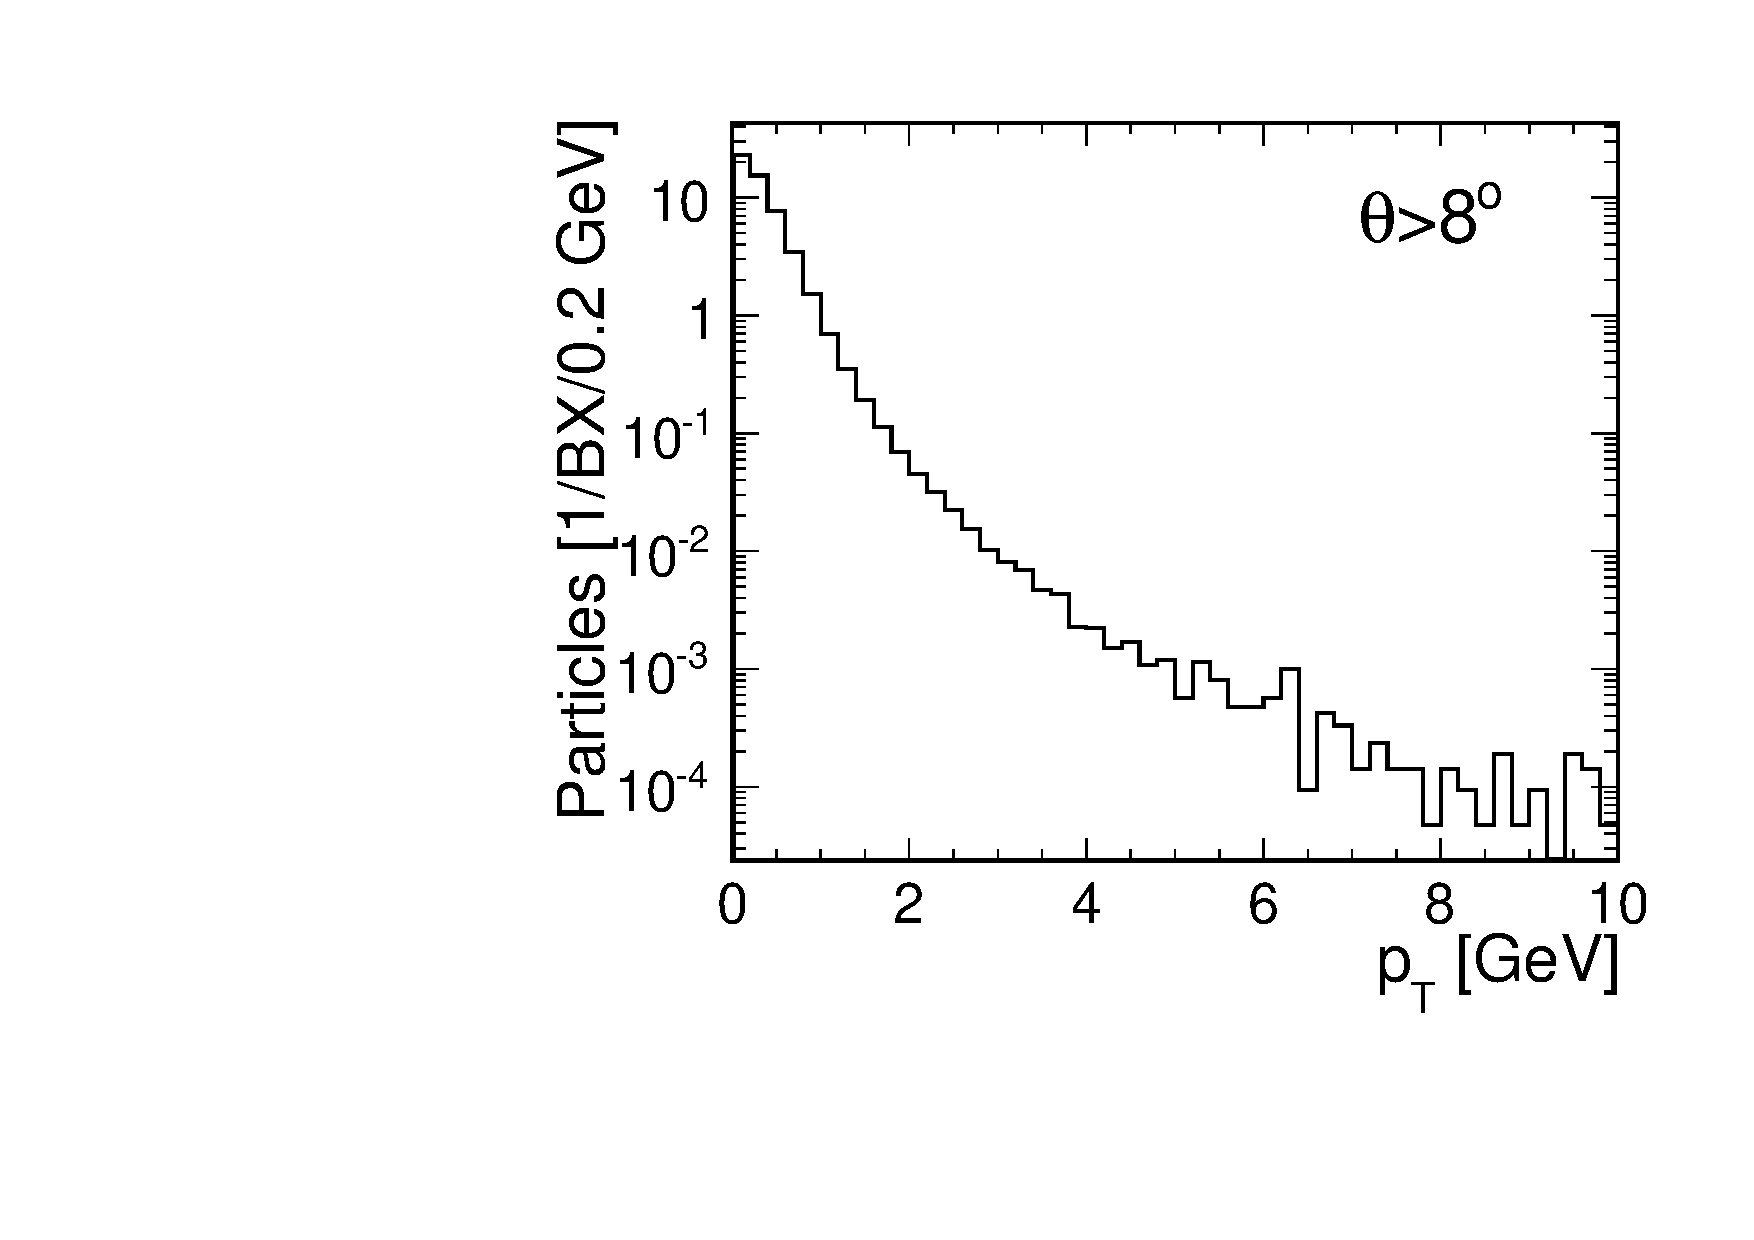
\includegraphics[width=0.49\linewidth]{../Chap3_ExpCond_PhysPerfsReqs/gghad-pt.pdf}
 \caption{The generated \pT distribution for particles from \gghadrons which are within a notional 
 detector angular acceptance of $8^\circ<\theta<172^\circ$. The rate
 is normalised to one bunch crossing, excluding safety factors for the simulation uncertainties.
 \label{fig:chap3:gghad-pt}}
\end{figure}



\subsubsection{Beam Halo Muons\label{sec:chapter3:environment:beamhalo}}

Machine-induced secondary electrons or positrons, produced, for example, from
inelastic collisions with the residual molecules in the beam pipe are a
potential source of detector background. The \acs{BDS} is designed to mitigate
the potential effects of this background, with six collimation stations placed
at strategic locations to ensure that essentially no beam particles are lost in
the last several hundred meters upstream of the \acs{IP}. 

High energy secondary muons are produced in inelastic collisions in the collimation of the beam halo 
electrons or positrons, and may reach the experimental cavern and the detector.
This beam halo muon background can be reduced significantly
through adaptations of the collimation scheme and through the placement of passive and/or
magnetised iron spoilers in the \acs{BDS}. Detailed tracking studies of the muons
through the \acs{BDS} have been performed. Preliminary results indicate that
it is realistic to aim for an average of 1 muon per 20 bunch crossings (combined from both beams) 
traversing the detector volume. Further information is given in~\cite{CLICacceleratorCDR}.
%For this report, one muon per BX is therefore assumed.

The simulated beam halo muon distribution in both energy and position has been used as the input to a number of 
dedicated detector simulation studies to assess the impact of this background.
For example, the occupancy in the \acs{TPC} due to halo muons 
was investigated, see Section~\ref{chapter_7_sect3}, and is
found to be negligible compared to the background from \gghadrons.

The beam halo muon background in the calorimeters can locally result in a significant energy deposition due to high energy 
electromagnetic showers produced by Bremsstrahlung. For an assumed single beam halo muon per bunch 
crossing -- a factor 20 above the expected halo muon rate -- the
average energy deposition for the entire bunch train would be approximately 3~TeV. 
Using the "tight" \acs{PFO} timing cuts (see Chapter~\ref{chapter_14}) this is reduced to approximately 100~GeV in time 
with a physics event. However, due to the highly granular nature of the proposed CLIC detector concepts, much of 
the remaining background can be rejected. A preliminary version of a 
pattern recognition algorithm, designed to remove hits and 
clusters consistent with coming from beam halo muons, was implemented in the \pandora reconstruction code.
It was demonstrated that the residual calorimeter background can be reduced to the level of approximately 10~GeV.
The impact of this background on physics observables was studied by overlaying a full bunch train of halo muons 
on $\ww \to \mathrm{qq} \PGm \PGn$ events at 1~TeV (a sample of \PW--like particles of 500~GeV mass decaying hadronically). 
%referring to Mark's presentation on 22 June 2011, see
%https://indico.cern.ch/getFile.py/access?contribId=0&resId=1&materialId=slides&confId=141893
For the background assumed for this study, one muon per BX (which implies a safety margin of a factor 20), 
the impact on the reconstructed
\PW mass distribution was found to be significantly less than that of the \gghadrons
background. 

In summary, at the expected level of 1 muon per 20 BX, the beam halo muon background does
not constitute an important problem for the detector concepts being
considered here, \ie in detectors which have sufficient granularity and timing
resolution in the calorimeters. 
%Further studies are needed on reducing the
%number of halo muons reaching the detector, as well as on mitigating their impact using more sophisticated
%pattern recognition algorithms.

\subsubsection{Backscattering from the Post-Collision Line and the Beam Dump\label{sec:chapter3:environment:backscattering}}

After collision, the particles are transported through a system of magnets -- 
the "post-collision line" -- to the main CLIC beam dump, 315~m downstream of the
\acs{IP}.
The beam-beam effect leads to a broad energy spectrum of electrons, positrons and photons,
some of which are lost in collimators installed to protect the magnets. Detailed Monte-Carlo simulations
have been performed in order to assess the particle flux scattering back from the post-collision line
towards the detector at the IP\@. The model includes the magnets, collimators, vacuum pipe, beam dump and tunnel walls,
but not the CLIC detector itself. Particles are counted in a scoring plane placed at 3.5~m from the IP.
The flux obtained in these simulations is approximately 20 photons (energies below 500~keV)
and 4 neutrons (energies below 1~MeV) per cm$^2$ and bunch train~\cite{EddaatIPAC11}. Adding the "self-shielding" effect of 
the CLIC detector yoke against such low energy particles, it can be concluded that backscattering from the 
post-collision line and beam dump is negligible.

\subsection{Beam Polarisation at CLIC\label{sec:chapter3:environment:polarisation}}
The CLIC accelerator conceptual design includes a source to produce a polarised electron beam,
and all elements necessary to transport the beam to the IP without loss of polarisation. 
An electron beam polarisation of 80\% is expected for the CLIC experimental programme. 
This corresponds to what is already achievable today for lower energy electron accelerators.   
   
Currently, a polarised positron beam is not part of the CLIC baseline, although provisions have been made
in the design of the accelerator complex to add this option at a later stage. 
Conservatively, one may assume 30\% polarisation of the positrons after such an upgrade phase.

The degree of polarisation in the beams can be measured in a dedicated section of the 
Beam Delivery System (\acs{BDS}) at CLIC, several hundred metres upstream of the IP,
using the well-established Compton back-scattering technique. 
Detailed studies performed for the 500~GeV beams at the ILC have been extrapolated to 
CLIC, and a statistical uncertainty of better than 0.1\% can be expected, 
even for low intensity beams during initial running of the accelerator complex
(cf. \acs{BDS} section in~\cite{CLICacceleratorCDR}).

Knowing with high absolute accuracy the degree of polarisation at the 
time of the interaction is important for a number of physics processes to be studied at CLIC\@. 
At 3~TeV centre-of-mass collision energy, this absolute accuracy is hampered by effects of the 
very strong beam-beam interaction. On the one hand, this produces a large number of beamstrahlung 
photons and coherent pairs. This creates a spray of background particles in the post-collision line, 
and makes it impossible to measure the beam polarisation after the IP\@. 
Moreover, the beam-beam interaction leads to depolarisation. 
Simulations indicate that the depolarisation varies throughout the luminosity spectrum~\cite{Bailey_2011, Esberg_2011}, 
starting below 1\% around the high energy peak at 3~TeV 
(i.e. for events with a lower degree of beam-beam losses) and reaching up to 4\% at the lower energies 
(i.e. where the beam-beam effects are strongest). 
The systematic uncertainty on the absolute degree of beam polarisation is therefore 
left to future detailed studies.


%%----------------------------------------------------------------------------------------------------------------------
%%Title cant use macro, or e+e- is not bolded like the rest of the title
\section{\texorpdfstring{Detector Requirements for $\mathbf{e}^{+}\mathbf{e}^{-}$ Physics in the
    TeV-Range}{Detector Requirements for e+e- in the TeV-Range}\label{sec:chapter3:detector_requirements}}

The detector requirements at a 500~GeV \epem collider have been established in
the context of the ILC~\cite{Aihara:2009ad,ildloi:2009}. Assuming a staged
approach for CLIC, with the possibility of the initial operation at ILC-like
energies, the minimal requirements for a detector at CLIC are that it must meet
the \acs{ILC} detector requirements. However, the detector must also be suitable
for physics at centre-of-mass energies up to 3~TeV\@. In addition, the detector
must be able to operate effectively in the CLIC machine environment. Here the
most challenging aspect is the 0.5~ns bunch structure combined with the background
from \gghadrons which results in a deposition of approximately 20~TeV of energy
in the calorimeters for the entire train of 312 bunches. This implies not only
excellent time resolution for all detector components, but also a highly
segmented calorimeter to keep individual cell occupancies to a manageable level.

Chapter~\ref{chapter_02} presents a wide range of \acs{BSM} physics scenarios which
define the possible goals of a high energy \epem collider such as CLIC\@. These
broad physics goals can be used to define the minimal requirements for the
performance of a detector at CLIC at 3~TeV. The possible BSM physics signatures
at 3~TeV can be broadly characterised as:
\begin{itemize}
 \item high multiplicity jet final states, for example, $\epem\rightarrow\HpHm \rightarrow \tbtb$;
 \item multi-jet final states and missing energy, such as $\epem\rightarrow\PSGcpDo\PSGcmDo\rightarrow\ww \PSGczDo\PSGczDo$ 
 or signatures for strong \acs{EWSB};
 \item leptons and missing energy, for example, $\epem\rightarrow\PSGm\PSGm\rightarrow\mpmm\PSGczDo\PSGczDo$;
 \item heavy flavour production, for example in $\epem\rightarrow \Ph \PGne\PAGne$ where $\Ph\rightarrow\bb$ or $\Ph\rightarrow\cc$; 
 \item exotic final states, for example, non-pointing photons in certain
 \acs{SUSY} \acs{GMSB} models.
\end{itemize} 
The main detector requirements for the reconstruction of physics events at CLIC are discussed below.


\subsection{Track Momentum Resolution\label{sec:chapter3:requirements:momentum}}

The track momentum goal at the ILC and CLIC is dictated by the Higgs mass determination
from the Higgsstrahlung process, $\epem \rightarrow \PZ\PSh$, where the mass can
be precisely reconstructed from the mass distribution of the system recoiling
against the pair of muons from $\PZ\rightarrow\mpmm$ decays. The precision of
the measurement is ultimately limited by the beam energy spread. For the
\acs{ILC} operating at 250~GeV and $m_{\PSh} = 120~\mathrm{GeV}$, the momentum resolution needs
to be $\sigma_{\pT}/\pT^2 \lesssim 5\cdot 10^{-5}~\mathrm{GeV}^{-1}$. For higher
centre-of-mass energies, where the muons have higher momenta, the requirements
are even more stringent. For example, the expected reconstructed recoil mass
distribution for $m_{\PSh}=120~\mathrm{GeV}$ with the CLIC beamstrahlung spectrum at
$\roots=500$~GeV is shown in Figure~\ref{fig:chap3:Higgs_mumu_momres_dependence} (left) for different
assumed momentum resolutions. Despite the relatively large tail from beamstrahlung in the recoil
mass distribution, a clear peak at the Higgs mass can be
observed. For the width to be dominated by the beam energy spread requires
$\sigma_{\pT}/\pT^2 \sim 2\cdot 10^{-5}~\mathrm{GeV}^{-1}$.

The track momentum requirement at $\roots=3~\mathrm{TeV}$ is also driven by the measurement
of the Higgs branching ratio to muons. An excellent mass resolution is crucial to distinguish
this rare decay from its background channels. Figure~\ref{fig:chap3:Higgs_mumu_momres_dependence} (right)
shows the statistical uncertainty of the cross section times branching ratio measurement
of the $\PSh \to \mpmm$ channel depending on the momentum resolution. The numbers are obtained from
a fast simulation study similar to the analysis presented in Section~\ref{sec:chap14_hmumu}, assuming
different constant momentum resolutions, independent of the particle momentum or angle.
The full simulation results are consistent. An average momentum resolution of a few
\unit[$10^{-5}$]{GeV$^{-1}$} is desirable. For even better momentum resolutions the result is limited
by the intrinsic statistical uncertainty due to the small number of events.

\begin{figure}[hbt]
\centering
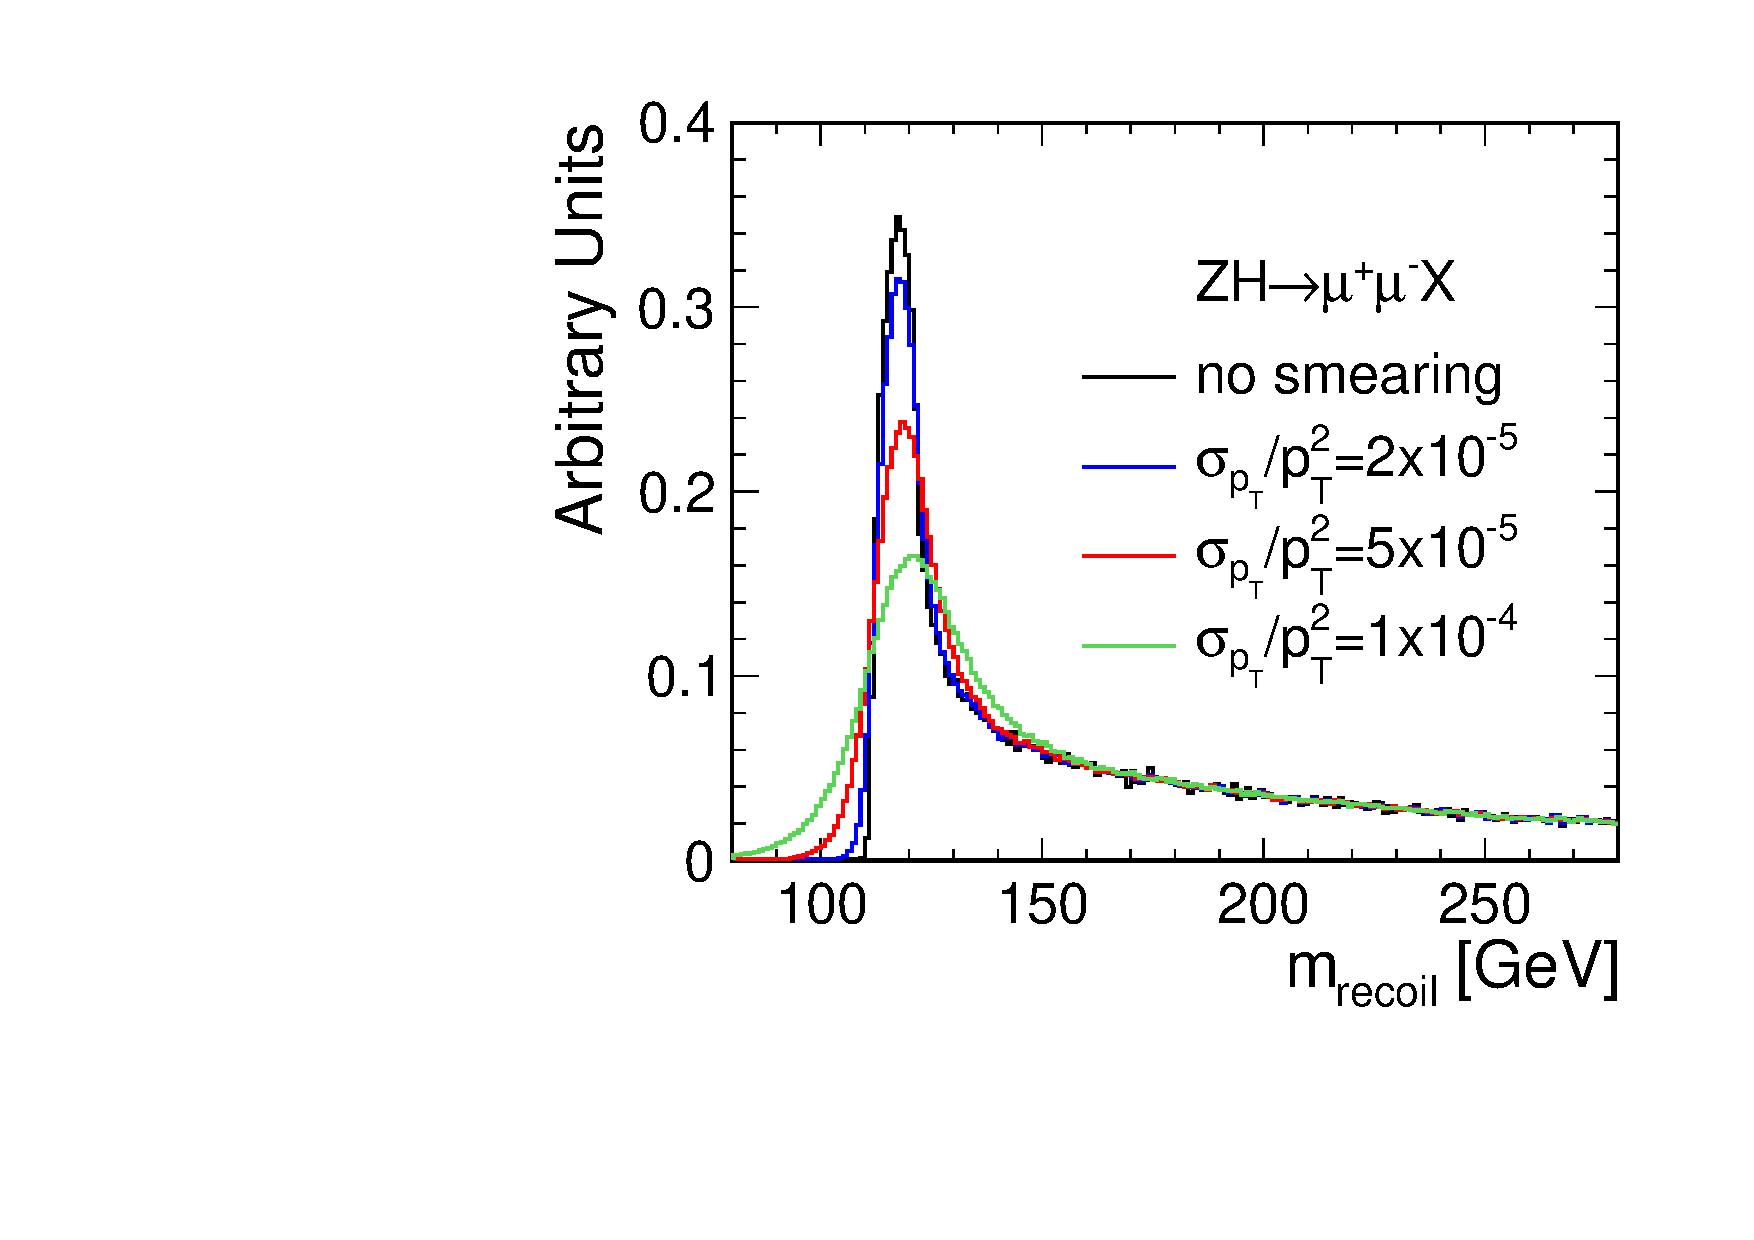
\includegraphics[width=0.49\linewidth]{../Chap3_ExpCond_PhysPerfsReqs/higgs.pdf} 
\hfill
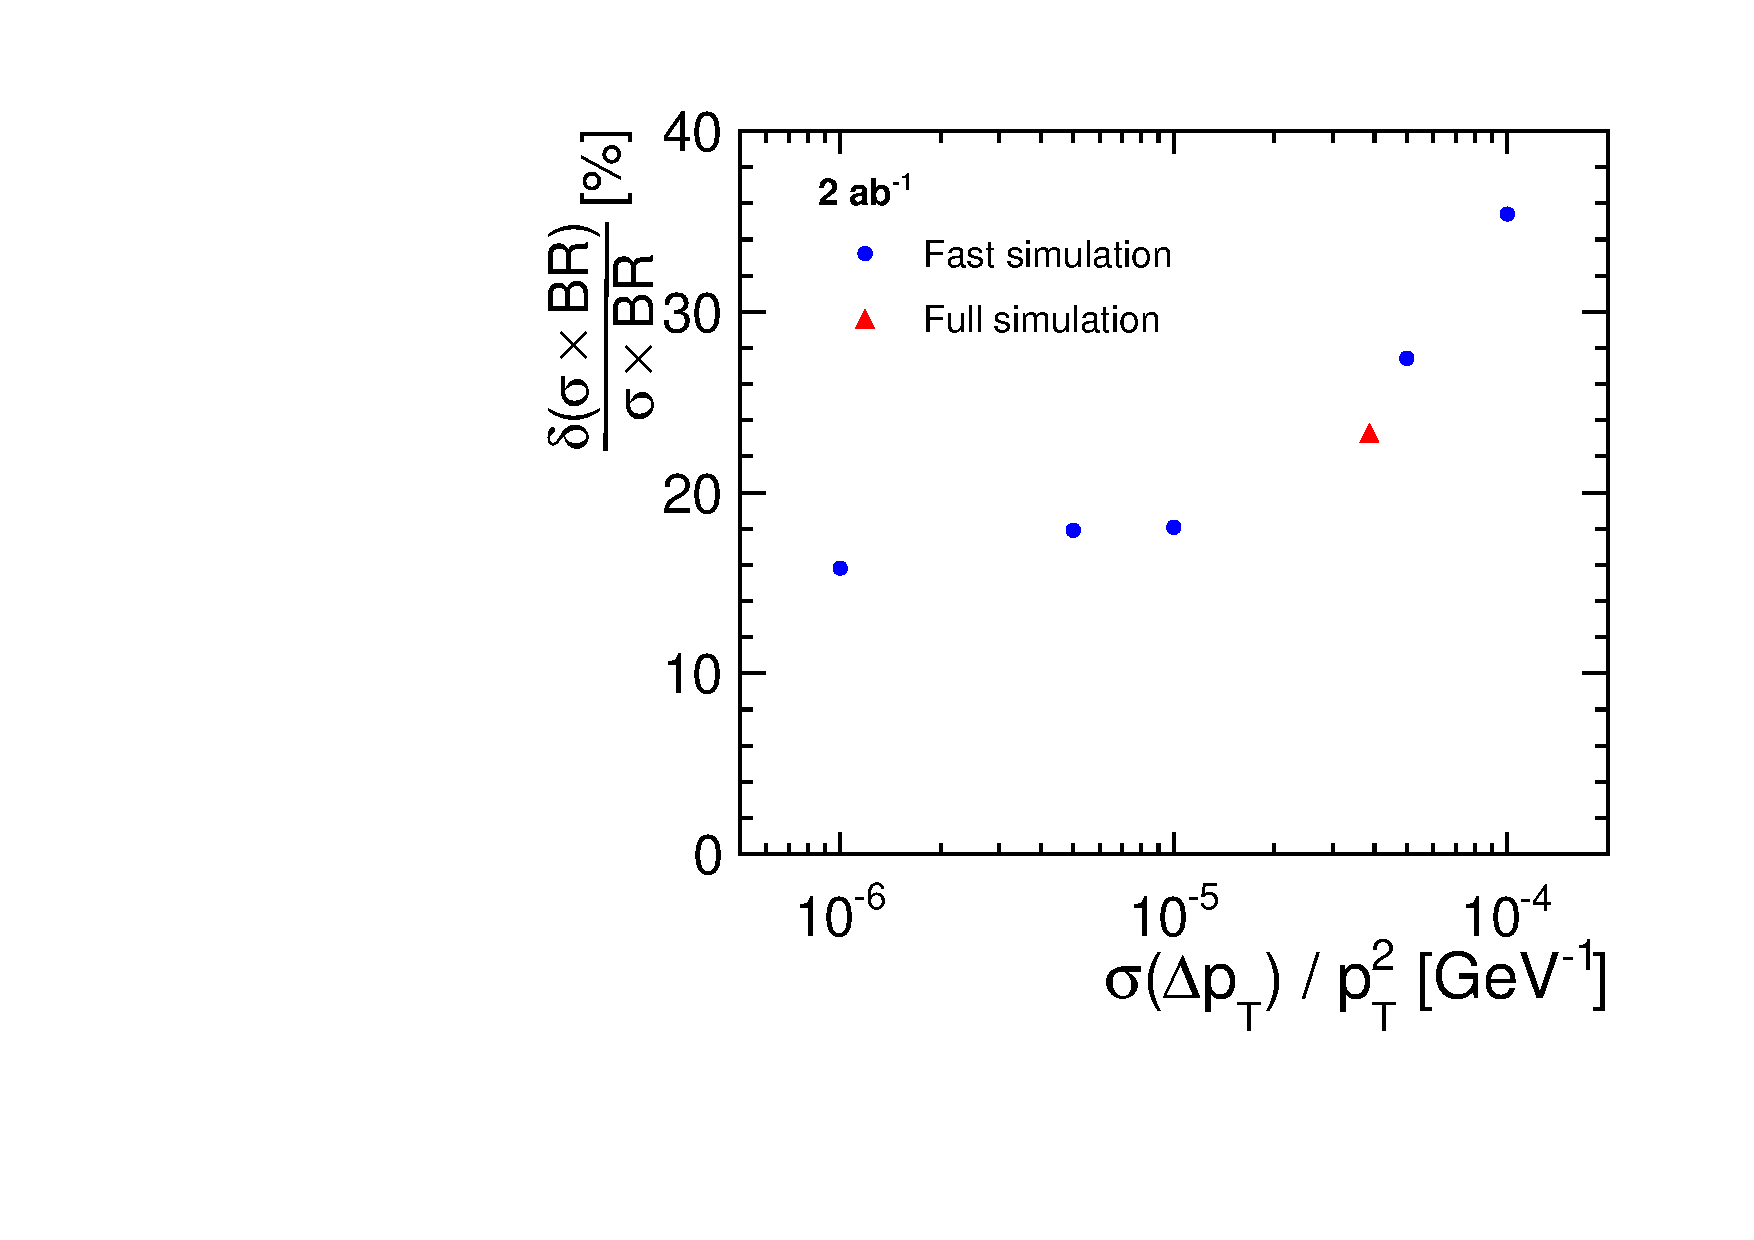
\includegraphics[width=0.49\linewidth]{../Chap3_ExpCond_PhysPerfsReqs/higgs_mumu_momres_dependence_2ab.pdf} 
\caption{Generator level reconstructed recoil mass distribution in the
Higgsstrahlung process $\epem\rightarrow\PZ\Ph\rightarrow\mpmm X$ from the
  muon momentum smeared by an assumed track momentum resolution (left). Statistical uncertainty 
  of the $\sigma\times\mathrm{BR}$ measurement of the $\PSh \to \mpmm$ channel
  depending on the momentum resolution (right). Results obtained from fast simulation are consistent with full simulation results.
  See Section~\ref{sec:chap14_hmumu} for details.
\label{fig:chap3:Higgs_mumu_momres_dependence}}
\end{figure}

Similar requirements on the momentum resolution ensue for several \acs{BSM} physics
scenarios. One possible example is the determination of the
smuon and neutralino masses from the muon momentum distribution in the process
$\epem\rightarrow\PSGm\PSGm\rightarrow\mpmm\PSGczDo\PSGczDo$.
Figure~\ref{fig:chap3:trackRequirements} (left) shows the generator level muon
momentum distribution from smuon decays (for the \acs{SUSY} \textit{model II} described in
the Section~\ref{sec:chapter3:benchmarks}) with different values for the assumed momentum
resolution. The high momentum part of the spectrum is significantly distorted
for a momentum resolution of $\sigma_{\pT}/\pT^2 >
4\cdot
10^{-5}~\textrm{GeV}^{-1}$. Figure~\ref{fig:chap3:trackRequirements} (right) shows the
corresponding reconstructed mass resolution for the neutralino and the smuon as
a function of momentum resolution.
\begin{figure}[hbt]
\centering
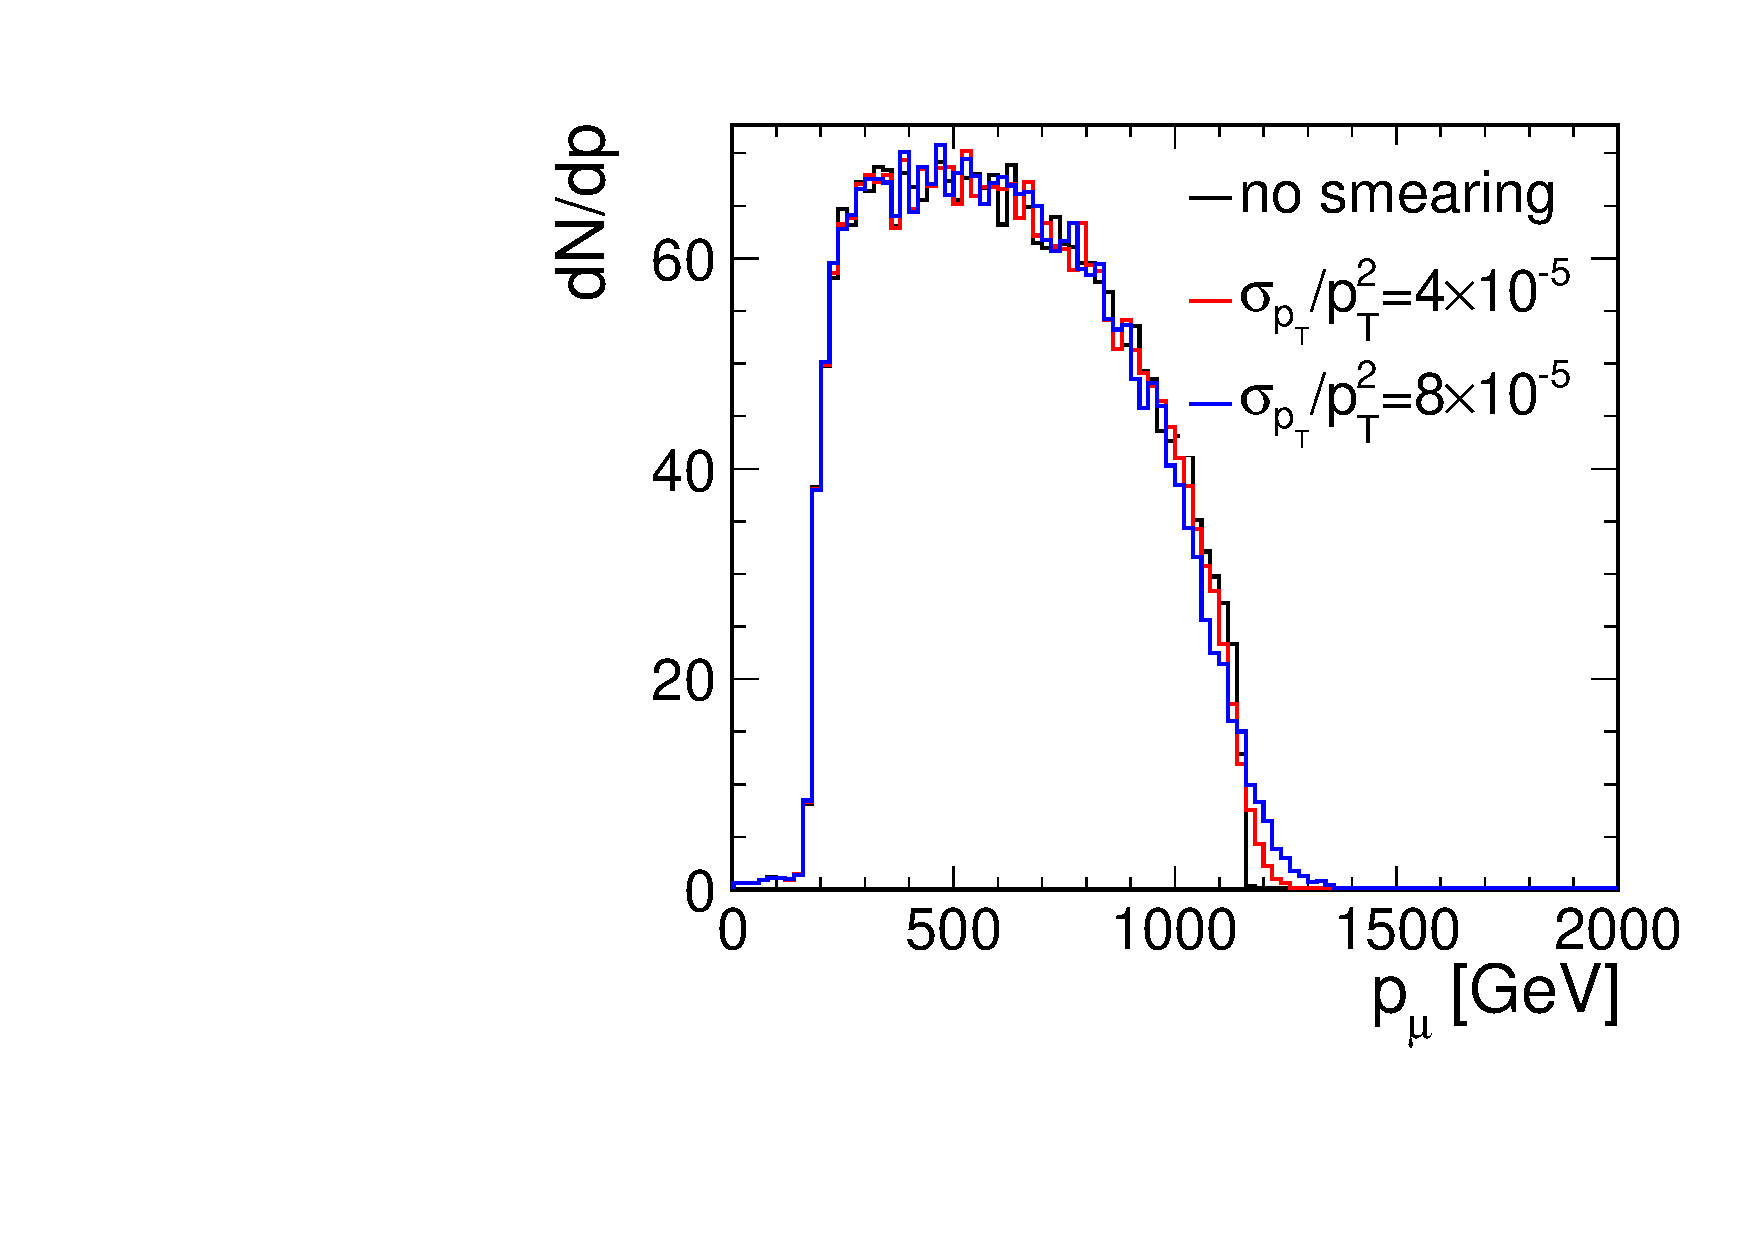
\includegraphics[width=0.49\linewidth]{../Chap3_ExpCond_PhysPerfsReqs/SleptonEndpoint.pdf} 
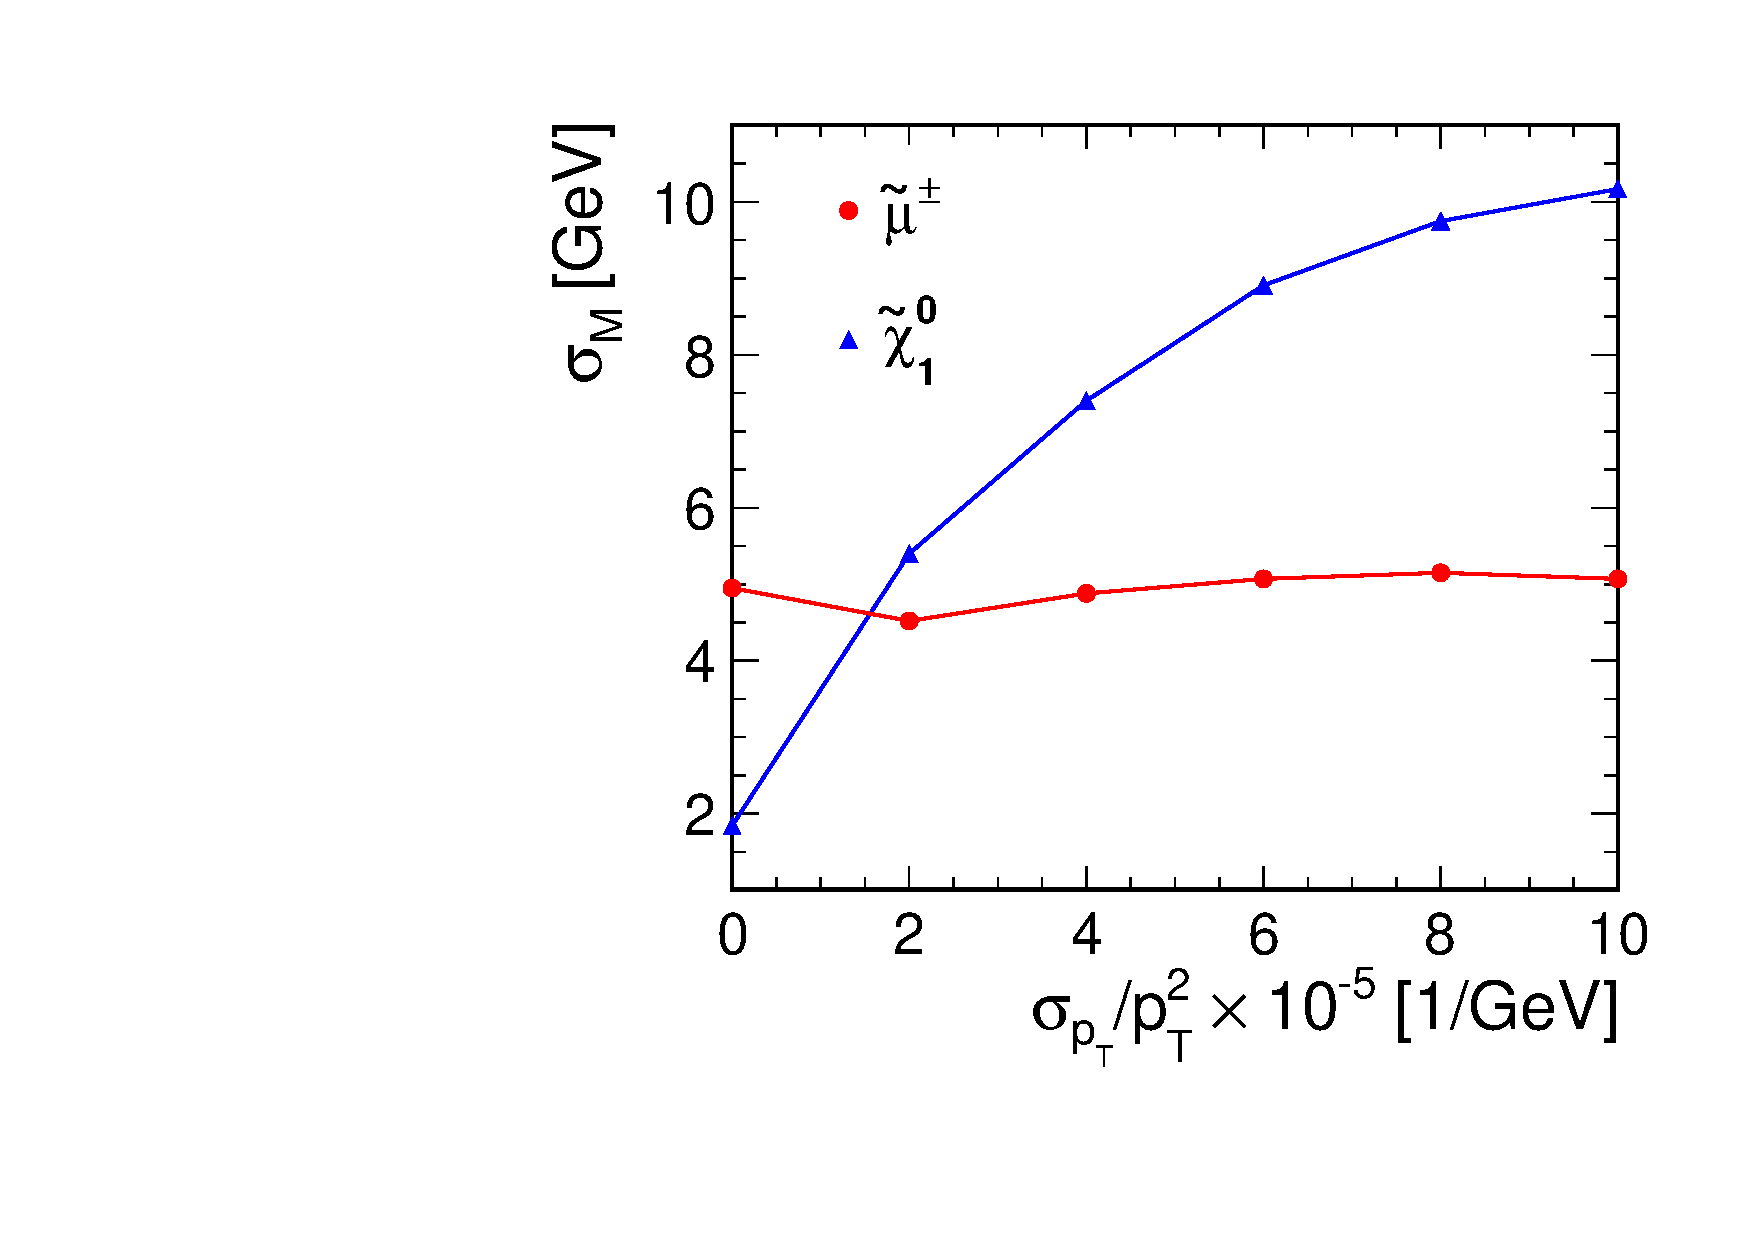
\includegraphics[width=0.49\linewidth]{../Chap3_ExpCond_PhysPerfsReqs/SleptonMassResolution.pdf}
\caption{(left) Generator level reconstructed muon momentum distribution for
  $\epem\rightarrow\PSGm\PSGm\rightarrow\mpmm\PSGczDo\PSGczDo$ assuming 2 \abinv
  of data at $\roots=3~\mathrm{TeV}$ in a SUSY model with $m(\PSGmL) =
  1100.4~\mathrm{GeV}$ and $m_{\tilde\chi_{1}^{0}}=328.3~\mathrm{GeV}$; (right)
  resolution on the reconstructed smuon and neutralino masses
  $\sigma_{\mathrm{M}}$ a function of the assumed momentum resolution
  $\sigma_{\pT}/\pT^{2}$. \label{fig:chap3:trackRequirements}}

\end{figure}


\subsection{Jet Energy Resolution\label{sec:chapter3:requirements:jetenergy}}

Many of the interesting physics processes at CLIC are likely to be characterised
by multi-jet final states, often accompanied by charged leptons or missing
transverse momentum associated with neutrinos or possibly the lightest super-symmetric
particles. The reconstruction of the invariant masses of two or more jets will
be important for event reconstruction and event identification. At \acs{LEP},
kinematic fitting enabled precise invariant mass 
reconstruction and reduced the dependence on the intrinsic calorimetric
performance of the \acs{LEP} detectors. At CLIC, due to beamstrahlung, kinematic
fitting will be, in general, less powerful and the di-jet mass reconstruction
will rely more heavily on the intrinsic jet energy resolution of the detector. 
One goal for jet energy resolution at CLIC is that it is sufficient to
provide discrimination between the hadronic decays of \PW and \PZ boson.
Figure~\ref{fig:chap3:jetRequirements} (left) shows idealised reconstructed \PW and
\PZ mass distributions for different assumed mass resolutions. Good separation is obtained for 
a mass resolution of 2.5\%, which corresponds to a jet energy resolution of
3.5\%. To obtain a separation
corresponding to $2.5\sigma$ implies a jet energy resolution of
$3.5\%$~\cite{thomson:pandora} for the entire range of jet energies of
interest at CLIC, \ie 50~GeV -- 1~TeV. A jet energy resolution of 5\% leads to a $2\sigma$  \PW/\PZ separation. 
The reconstruction of mass-related
variables in \acs{BSM} decays such as $\PSQR\rightarrow\PQq\PSGcz$ will also benefit
from good jet energy resolution. Figure~\ref{fig:chap3:jetRequirements} (right) shows
the distribution of the contravariant mass,
$M^2_{\mathrm{C}}=2(E_1E_2+\vec{p}_1\cdot\vec{p}_2)$, in
%$M^2_{\mathrm{C}}=(E_1+E_2)^2-(\vec{p}_1-\vec{p}_2)^2$ in  %%% MAT - I think this is the correct form 
$\epem\rightarrow\PSQR\PASQR\rightarrow\PQq\PSGcz\PAQq\PSGcz$, where $E_{1,2}$
and $\vec{p}_{1,2}$ are the reconstructed energies and momenta of the two jets~\cite{LCD-2010-012}.
The location of the high mass edge can be used to determine the mass
difference between the \PSQR and the \PSGcz. The sharpness is determined by
both the underlying beamstrahlung spectrum and the jet energy resolution. For
$\sigma_E/E$ of $<5\%$, the measurements are dominated by the effects of
beamstrahlung rather than the jet energy resolution.
\begin{figure}[hbt]
\centering
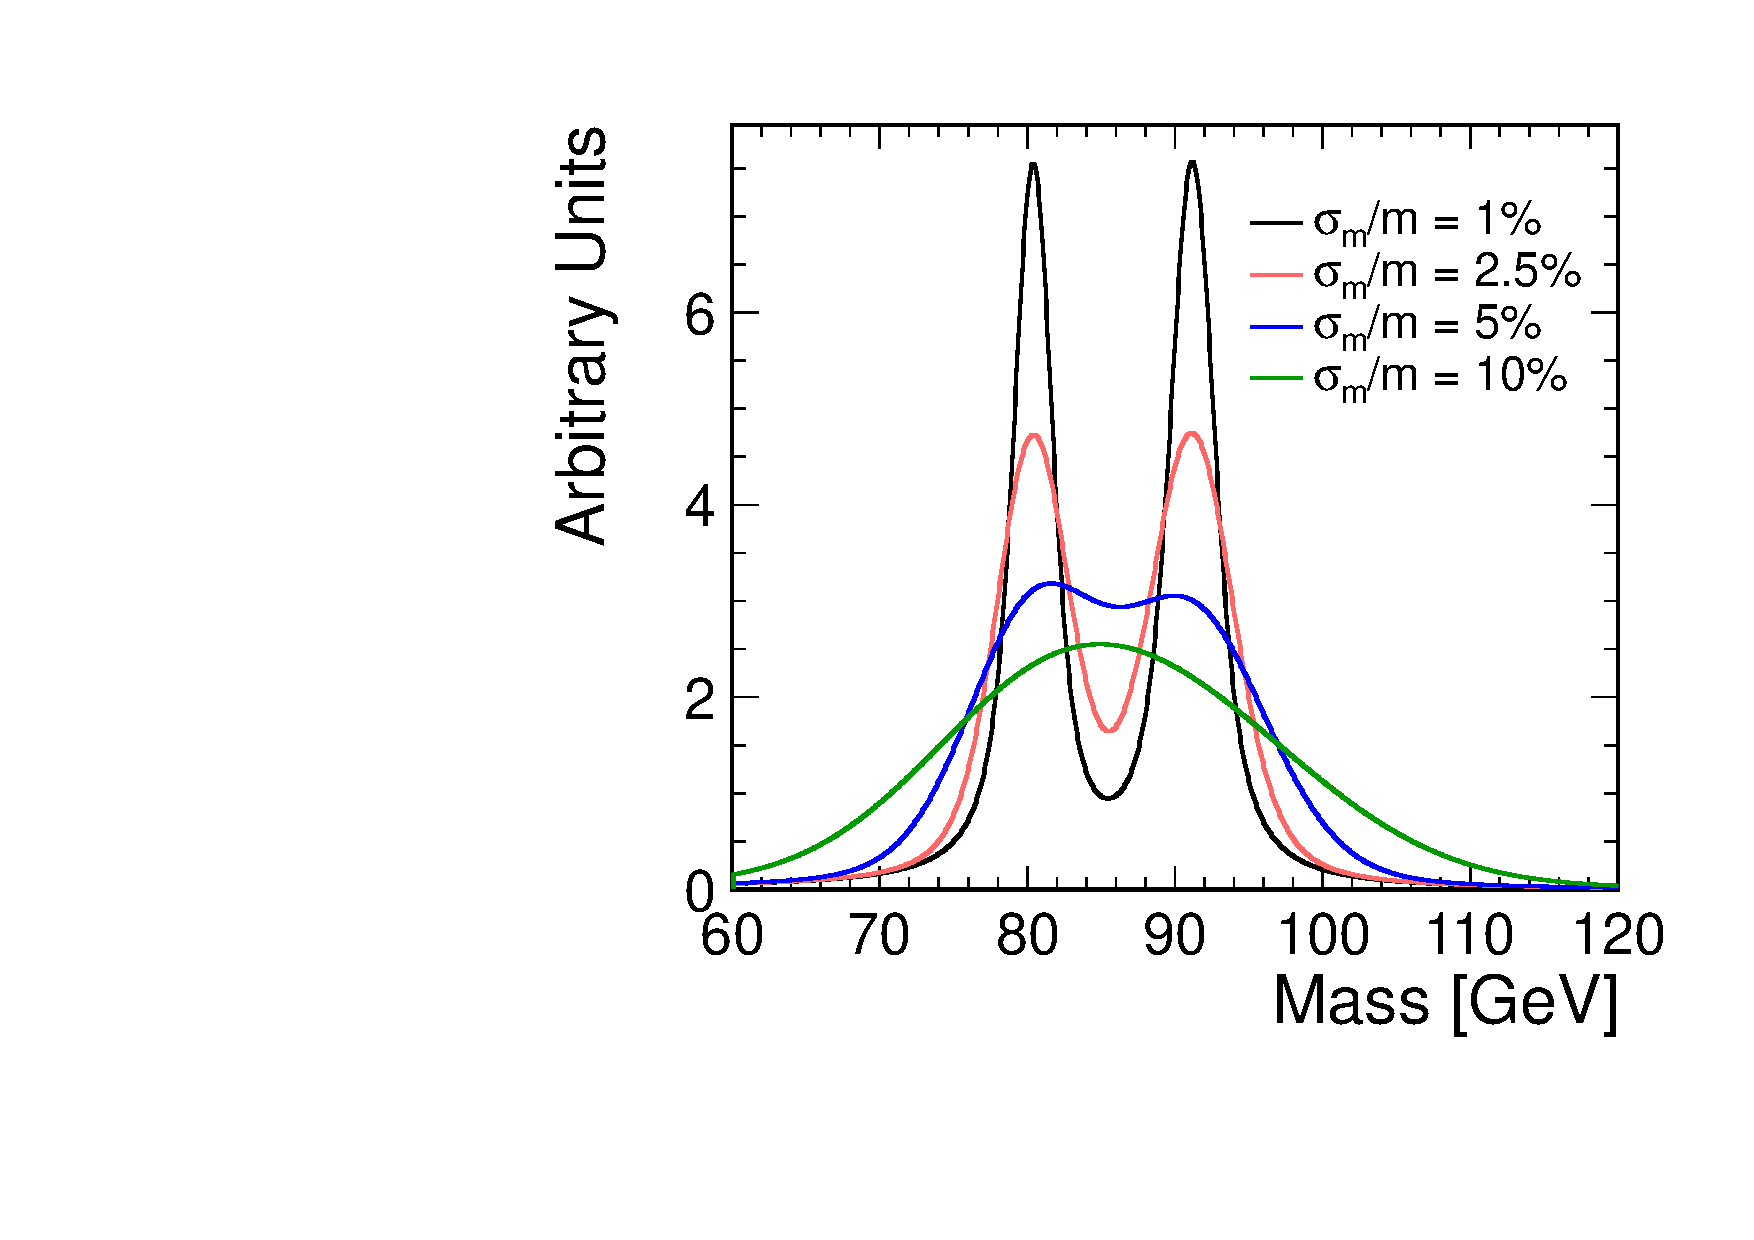
\includegraphics[width=0.49\linewidth]{../Chap3_ExpCond_PhysPerfsReqs/wzSeparation.pdf}
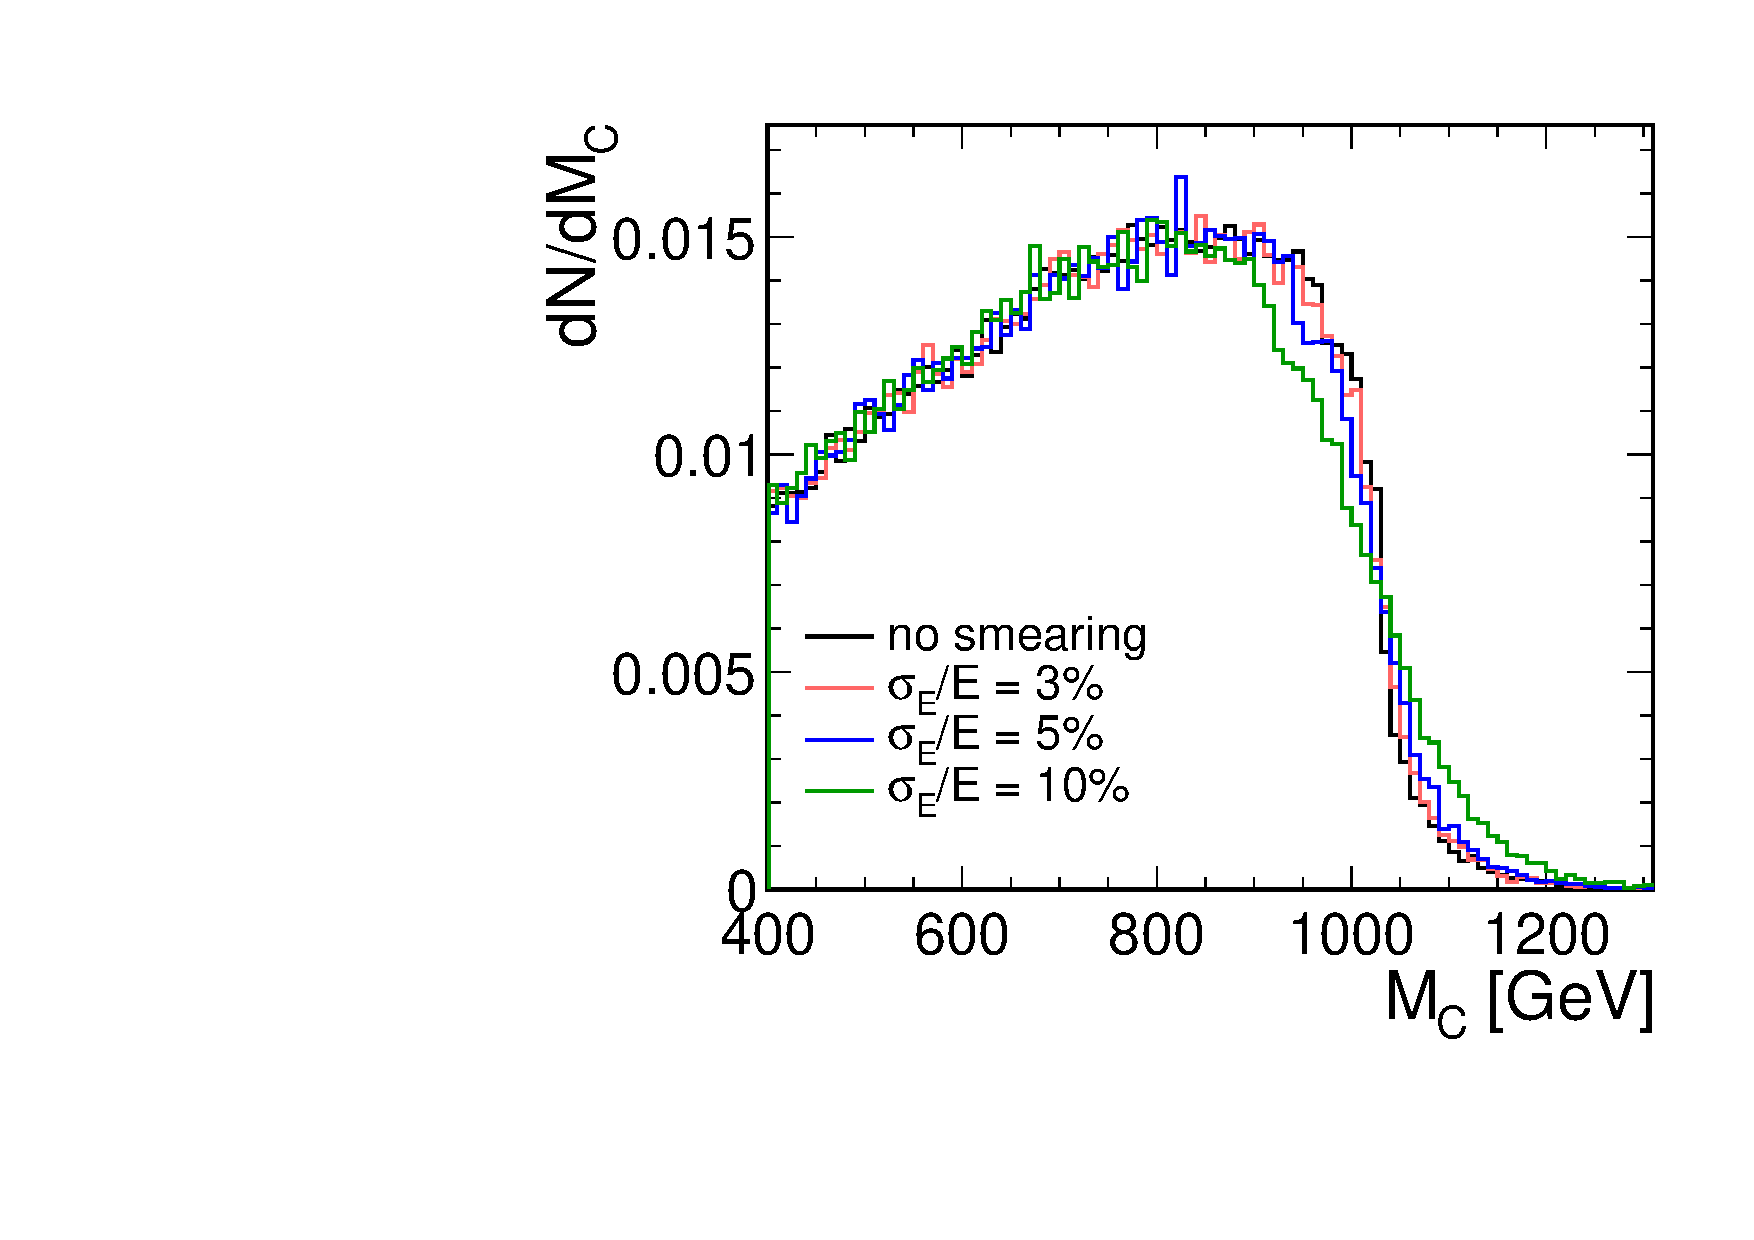
\includegraphics[width=0.49\linewidth]{../Chap3_ExpCond_PhysPerfsReqs/SquarkEndpoint.pdf}
\caption{(left) Ideal \PW/\PZ separation vs.\ jet mass resolution obtained using
a Gaussian smearing of Breit-Wigner distributions; (right) Reconstructed
contravariant mass, $M_\mathrm{C}$, for
$\epem\rightarrow\PSQR\PASQR\rightarrow\PQq\PSGcz\PAQq\PSGcz$ (including the
effects of Beamstrahlung) for different jet energy resolutions. The plot was
obtained by applying a Gaussian energy smearing to reconstructed jets based on
the generator level particles.  \label{fig:chap3:jetRequirements}}

\end{figure}

\subsection{Impact Parameter Resolution and Flavour Tagging\label{sec:chapter3:requirements:flavourtagging}}

Whatever the physics at CLIC, the ability to efficiently tag b-quarks will
feature in many physics studies. For CLIC operating in the energy range between $\roots=500$~GeV and $\roots=3$~TeV, it is
likely that one of the main physics goals will be the measurement of the 
couplings of the Higgs. Here the ability to tag both charm and bottom quarks
will be important. High performance flavour tagging depends on the ability to
identify secondary vertices and tracks which do not originate from the IP\@. The
impact parameter resolution can be expressed in the form
\begin{equation}\label{chap3:eq:impactpararesolution}
\sigma_{d_{0}}^2 = a^2 + \frac{b^{2}}{p^{2}\sin^{3}\theta}~,
\end{equation}
where the constant $a$ depends on the point resolution of the vertex detector and
parameter $b$ is related to multiple scattering and thus depends on the
amount of material in the inner detector and the geometrical arrangement of the
layers. The target values for a detector at
CLIC are derived from those for the \acs{ILC}~\cite{ildloi:2009}, 
namely $a  \lesssim 5~\micron$ and
$b \lesssim 15~\mathrm{\micron~GeV}$. 
% In the ILD LOIs the target was b<10 um. But we can not reach this, due to the larger
% beam-pipe radius. Also, SiD reached only b<~15 um in the LOI simulations.
This represents a factor 2--3 improvement
with respect to the \acs{SLD} vertex detector, both in terms of point resolution and
material budget. For CLIC operating at $\roots=3~\mathrm{TeV}$, efficient flavour
tagging will be essential for final states containing multiple \PQb-jets.

\subsection{Forward Coverage\label{sec:chapter3:requirements:forward}}
At CLIC many \acs{SM} processes will result in particles produced at relatively low angles to the beam axis; either
due to the boost along the beam axis from beamstrahlung or from $t$-channel processes. To study these processes, on the one hand, or to reduce their impact on \acs{BSM} physics studies, on the other hand, extending the detector coverage to small
polar angles is important~\cite{Fuster:2009em}.

For example, at 3~TeV, approximately 80\% of the leptons
in the \llll final state, dominated by gauge boson pairs, are produced at polar angles of $<30^\circ$ to the beam axis.
The forward region is also important for physics signatures with missing energy. It helps to reject background processes like
multi-peripheral two photon processes, $\epem \to \epem f\bar{f}$, where the scattered electrons are usually at low polar angles.
For example, forward electron tagging is essential to reject the $\epem \to \epem\mpmm$ background in the measurement of the Higgs branching ratio into two muons.
As shown in Chapter~\ref{sec:chap14_hmumu}, it improves the achievable statistical accuracy of this measurement from 23\% to 15\%, assuming an integrated luminosity of 2~\abinv and 95\% electron tagging efficiency down to $\approx$ 40~mrad polar angle.
Another example is the production and decay of stau pairs, $\epem\rightarrow\PSGt\PSGt\rightarrow\tptm\PSGczDo\PSGczDo$,
which, in some regions of \acs{SUSY} parameter space, results in a signal with relatively small missing transverse momentum.
In this case, the $\epem \to \epem\tptm$ and $\epem \to \epem\qqbar$ background processes need to be rejected by efficient
electron tagging at low polar angles. It is therefore important, in general, to provide precision tracking and calorimetry coverage down to small angles, and to extend the forward electron tagging capabilities to very low angles.

\subsection{Lepton ID Requirements\label{sec:chapter3:requirements:leptonID}}

Many of the potential \acs{BSM} physics signals at CLIC will rely on the ability to
efficiently identify high energy electrons and muons, and
efficient lepton identification is central to the CLIC detector requirements.
For efficient selection of final states with two or more leptons, lepton
identification efficiencies of more than 95\% over a wide range of momenta are highly
desirable. In addition the identification of leptons in jets from
semi-leptonic decays of \PQb- and \PQc-quarks will benefit heavy flavour tagging.

\subsection{Summary of Requirements for Physics Reconstruction}

From the perspective of the likely physics measurements at CLIC the detector requirements are:
\begin{itemize}
 \item jet energy resolution of $\sigma_E/E \lesssim 3.5-5\%$ for jet energies in the
 range 50~GeV -- 1~TeV;
 \item track momentum resolution of $\sigma_{\pT}/\pT^2 \lesssim
   2\cdot 10^{-5}~\textrm{GeV}^{-1}$;
%%not using eqref to avoid double parenthesis
 \item impact parameter resolution (equation
   \ref{chap3:eq:impactpararesolution}) with $a \lesssim 5~\micron$ and $b \lesssim 15~\micron\,\mathrm{GeV}$;
 \item lepton identification efficiency: $>95\%$ over the full range of energies; 
 \item detector coverage for electrons down to very low angles. 
\end{itemize}


%%----------------------------------------------------------------------------------------------------------------------

\section{Basic Choice of Detector Concepts for CLIC\label{sec:chapter3:concepts}}

The design considerations driving the basic choice of the detector concept(s)
for CLIC are clear; excellent track momentum and jet energy resolution,
excellent flavour tagging capability and the ability to perform precision
physics measurements in the CLIC background environment. This in turn implies
excellent time stamping capability for all detector elements. It is the jet energy 
resolution in the relatively high background environment that
has the largest impact on the overall design of a detector concept for CLIC.

Traditionally, jet energies have been obtained from the sum of the energies deposited 
in the electromagnetic and hadronic calorimeters (ECAL and HCAL) giving a jet energy 
resolution of the form
\begin{eqnarray*}
  \frac{\sigma_E}{E} &=& \frac{\alpha}{\sqrt{E\mathrm{(GeV)}}} \oplus \beta. \label{eqn:cal} 
\end{eqnarray*}
The stochastic term $\alpha$ is usually greater than 60\% and the
constant term $\beta$, which encompasses a number of effects, is typically
a few per cent. For high energy jets there also will be a contribution 
from the non-containment of the hadronic showers. 
To achieve the CLIC goal of a jet energy resolution of $\sim$3.5\% or better would require
a stochastic term below 30\% and a small constant term. 
This is unlikely to be achievable with a traditional approach to calorimetry. 
Calorimetry at a future lepton collider has been studied extensively in the
context of the ILC; it is widely acknowledged that high granularity particle flow
calorimetry is currently the most promising approach to achieving a jet energy resolution
of 3.5\%~\cite{pfaBrient, pfaMorgunov, thomson:pandora}.
High granularity particle flow calorimetry is also well suited to the relatively
high levels of background; it has the potential to separate calorimetric
energy deposits from background particles from those of the hard interaction.

Depending on the staging of the machine any detector must meet the physics requirements over
a range of centre-of-mass energies, 0.5~TeV -- 3.0~TeV. Over the last decade
concepts for general purpose detectors which meet the physics requirements for the \acs{ILC}
operating at $\roots=500~\mathrm{GeV}$ have been developed. In particular two detector
concepts, \acs{ILD}~\cite{ildloi:2009} and \acs{SiD}~\cite{Aihara:2009ad}, both based on high
granularity particle flow calorimetry, have been studied in detail. Modified versions
of these detector concepts (\clicild and \clicsid) form the basis of the
detector concepts for CLIC as discussed in detail in Chapter~\ref{chapter_05}. 

\subsection{The Particle Flow Paradigm\label{sec:chapter3:concepts:pfa}}

On average, after the decay of short-lived particles, roughly 60\% of the jet
energy is carried by charged particles (mainly hadrons), around 30\% by
photons, and about 10\% by long-lived neutral hadrons (\eg \Pn, \PAn and
\PKL). In contrast to a purely calorimetric measurement, particle flow
calorimetry requires the reconstruction of the four-vectors of all visible
particles in an event. The reconstructed jet energy is the sum of the energies
of the individual particles. The momenta of charged particles are measured in
the tracking detectors, while the energy measurements for photons and neutral
hadrons are obtained from the calorimeters. In this manner, the HCAL is used to
measure only about 10\% of the energy in the jet. If one were to assume
calorimeter resolutions of $\sigma_E/E = 15\%/\sqrt{E\mathrm{(GeV)}}$ for photons
and $\sigma_E/E = 55\%/\sqrt{E\mathrm{(GeV)}}$ for hadrons, a jet energy resolution
of $19\%/\sqrt{E\mathrm{(GeV)}}$ would be obtained. In practice, this level of
performance is not reachable as it is not possible to perfectly associate all
energy deposits with the correct particles. This \textit{confusion} rather than
calorimetric performance is the limiting factor in particle flow calorimetry. Thus, the
crucial aspect of particle flow calorimetry is the ability to assign
calorimeter energy deposits to the correct reconstructed particles. This places
stringent requirements on the granularity of the \acs{ECAL} and \acs{HCAL}\@. From the point
of view of event reconstruction, the sum of calorimeter energies is replaced by
a complex pattern recognition problem, namely the Particle Flow reconstruction
Algorithm (PFA). Based on detailed simulations of the ILC detector concepts
using the \pandora particle flow reconstruction algorithm it has been
demonstrated that jet energy resolutions of approximately 3\% can be achieved for jet
energies in the range 100~GeV -- 1000~GeV~\cite{thomson:pandora,Marshall:2010}. 

It should be noted that whilst high granularity particle flow calorimetry is a
relatively new concept, energy flow and particle flow have been used
successfully by a number of collider experiments. \acs{OPAL}, \acs{DELPHI}, H1 and D\O\ obtained
improved jet energy resolution using the Energy Flow approach, whereby energy
deposits in the calorimeters are removed according to the momentum of
associated charged particle tracks. \acs{ALEPH} and, more recently, \acs{CMS} used particle
flow techniques~\cite{Aleph-jet,PFT-09-001,PFT-10-002,PFT-10-003} to attempt to reconstruct the four
momenta of the particles in an event. 

\subsubsection{Advantages of High Granularity Calorimetry at CLIC}

The argument for a high granularity detector for the ILC is based almost
entirely on the jet energy resolution requirements. This argument still holds at
CLIC\@. However, for a detector at CLIC there is an additional argument for very
high granularity calorimetry. At CLIC the hadronic shower development time
is longer than the 0.5~ns bunch spacing, the calorimeters
necessarily integrate over a number of bunch crossing (discussed in detail in
Section~\ref{sec:chapter3:clic_detector:physicsReconstruction}). Consequently the
calorimeters integrate over a few tens of bunch crossings of background from hadronic
two-photon events (\gghadrons). Reduction of this
background relies on the ability to temporally and spatially separate energy
depositions from the background from those from the physics interaction of
interest. The excellent spatial resolution of a high granularity calorimeter
designed for particle flow will provide significant additional benefit in the
reduction of this background.


\subsection{Detector Design Considerations\label{sec:chapter3:concepts:design}}

%%Describe in a few words the impact of the PFA choice on tracking, calorimeters, location of coil, segmentation etc.

The adoption of high granularity particle flow calorimetry significantly impacts the design of the detector at CLIC:
\begin{itemize}
 \item {\bf ECAL}: the ECAL segmentation has to be sufficient to resolve energy
 depositions from near by particles in high energy jets. Studies performed in
 the context of the \acs{ILC}~\cite{thomson:pandora,ildloi:2009} suggest a calorimeter
 transverse segmentation of $5\times5~\mathrm{mm}^2$ with approximately 30 longitudinal samplings.
 \item {\bf HCAL}: the HCAL segmentation has to be sufficient to resolve energy
 depositions from hadronic showers from different particles. Previous
 studies~\cite{thomson:pandora,ildloi:2009} suggest an analogue HCAL calorimeter
 transverse segmentation of at most $3\times3~\mathrm{cm}^2$ with approximately 50
 longitudinal samplings. The high degree of longitudinal samplings makes it
 possible to track particles through the HCAL\@. The HCAL also needs to be
 sufficiently thick, about 7.5 \lambdaint, to contain the majority of the energy 
 from high energy jets at CLIC.
 \item {\bf Solenoid}: for the purposes of particle flow reconstruction, the
ECAL and HCAL have to be on the inside of the solenoid. A high magnetic
field 
%%(at least 4~T) MAT can't justify this number 
is required to achieve the desired momentum resolution
and to separate tracks from nearby particles in high energy jets.
%%MAT - don't mix the arguments (moved text below)
%%A high field
%%is also beneficial from the point of view of particle flow calorimetry as it
%%tends to increase the mean distance between energy depositions in the
%%calorimeters from neutral and charged particles.
\item Overall detector geometry: to increase the separation of particles in the
calorimeters a large inner radius for the calorimeters is beneficial although
this can, to some extent, be compensated for by a higher magnetic field which
tends to increase the mean distance between energy depositions in the
calorimeters from neutral and charged particles~\cite{thomson:pandora}.
\end{itemize}
In addition to the above considerations, a detector at CLIC must meet the requirements outlined in 
Section~\ref{sec:chapter3:detector_requirements}.
 

%%----------------------------------------------------------------------------------------------------------------------

\section{Detector Requirements for CLIC\label{sec:chapter3:clic_detector_requirements}}

The modified versions of the ILC detector concepts certainly meet the main
physics performance requirements for CLIC\@. However the CLIC experimental
environment is more challenging than that of the ILC and previous \epem
colliders. In particular, the detector must be able to cope with the relatively
high levels of background, which in turn dictates the timing and readout
requirements for the detector subsystems. Since the background increases with the
centre-of-mass energy, the majority of the following discussion focuses on
$\roots=3$~TeV where the background is most challenging.

\subsection{Impact of Backgrounds\label{sec:chapter3:clic_detector:background_impact}}

The main backgrounds in the CLIC detector are from incoherent pairs and
particles from \gghadrons. Particles from incoherent pairs are the dominant
backgrounds in the vertex and in the forward region. The particles from
\gghadrons are less forward-peaked and the dominant source of background in the
main tracking detectors and in the calorimeters (except at low radii in the
endcaps). Whilst the underlying background event rates can be determined from the
simulation of the beam alone, the backgrounds in the detector depend on the
exact detector design, in particular, on the detailed design of the forward
region. The background from incoherent pairs has two components, the particles
from the interaction point and backscattered particles from interactions in the
very forward region (particularly in the \acs{BeamCal}) and in the beam pipe
itself. The BeamCal is used as an active absorber and provides shielding to
nearby elements of the beam delivery system including the final focus
quadrupole. Whilst the detector is designed to minimise the backscattered
background, it is not possible to eliminate it completely.

To assess the levels of background in the main detector components it is
necessary to simulate the entire detector. For this purpose, the BeamCal and
beam pipe in the \clicild and \clicsid detector models were optimised to
minimise the backscattered
backgrounds in the vertex detector~\cite{lcd:2011-DannheimSailerBgrNote}. The background studies
described below were obtained for \geant models of the \clicild detector concept
with simulations performed for a full bunch train of incoherent pair and
\gghadrons backgrounds. The results for the \clicsid detector are not expected
to differ greatly.

\subsubsection{Impact on the Vertex Detector}  

In the absence of other constraints the inner layer of the vertex detector would
be placed at as small a radius as possible to the beam axis. In practice the
minimum radius is limited by the envelop of electrons and positrons from the
incoherent pair background. The higher \pT component of the pair background is
relatively low in energy and the background particles have helical trajectories
in the magnetic field of the detector. The dense core of pair-background
particles must not intercept the material of the detector as the resulting
interactions would result in a large source of background in the detector
volume. This restricts the minimum inner radius of the vertex detector to be
approximately 30~mm. The pair background also determines the locations of the
forward tracking discs. These constraints and the resulting backgrounds in the
vertex detector and forward tracking discs are discussed in detail in
Section~\ref{sec:vtx-hit-densities}.

\subsubsection{Impact on the Central Tracking Detector}  

The main background in the central tracking detector is due to relatively high
\pT tracks from \gghadrons interactions. There are approximately 3.2~\gghadrons events
per bunch crossing and each event results in an average of approximately 5
tracks which are reconstructable in the central tracking detector\footnote{Here
  reconstructable is defined as $\theta>8^\circ$ from the beam axis,
 and  $\pT>250~\mathrm{MeV}$.}. The mean
momentum of these tracks, which are forward peaked, is 1.5~GeV, resulting in a
charged particle background with total momentum of 24~GeV per bunch
crossing. Integrated over the 312 bunch crossings in the train there are over
5000 charged particle tracks with a total momentum of 7.3~TeV. The impact of
this background on the occupancy in the tracker and the resulting track finding
efficiency will depend strongly on the choice of technology used for the central
tracking device. This is discussed in detail in Chapter~\ref{chapter_07}.

\subsubsection{Backgrounds in the ECAL and HCAL}

The total energy deposition in the calorimeters from \gghadrons would be
expected to be approximately twice that observed in the central tracker. 
Figure~\ref{fig:chap3:caloBackEnergy} shows the energy depositions of the hits
in the \clicild ECAL and HCAL endcaps from an entire bunch train. In the ECAL
the contribution from \gghadrons dominates and a clear \acs{MIP} peak at just below
200~keV can be seen from both background sources. In the HCAL endcaps the
background arising from incoherent pairs dominates; this background originates 
mostly from low energy neutrons which arise from
interactions of the large incoherent pair background in the low angle BeamCal. 


\begin{figure}[hbt]
\centering
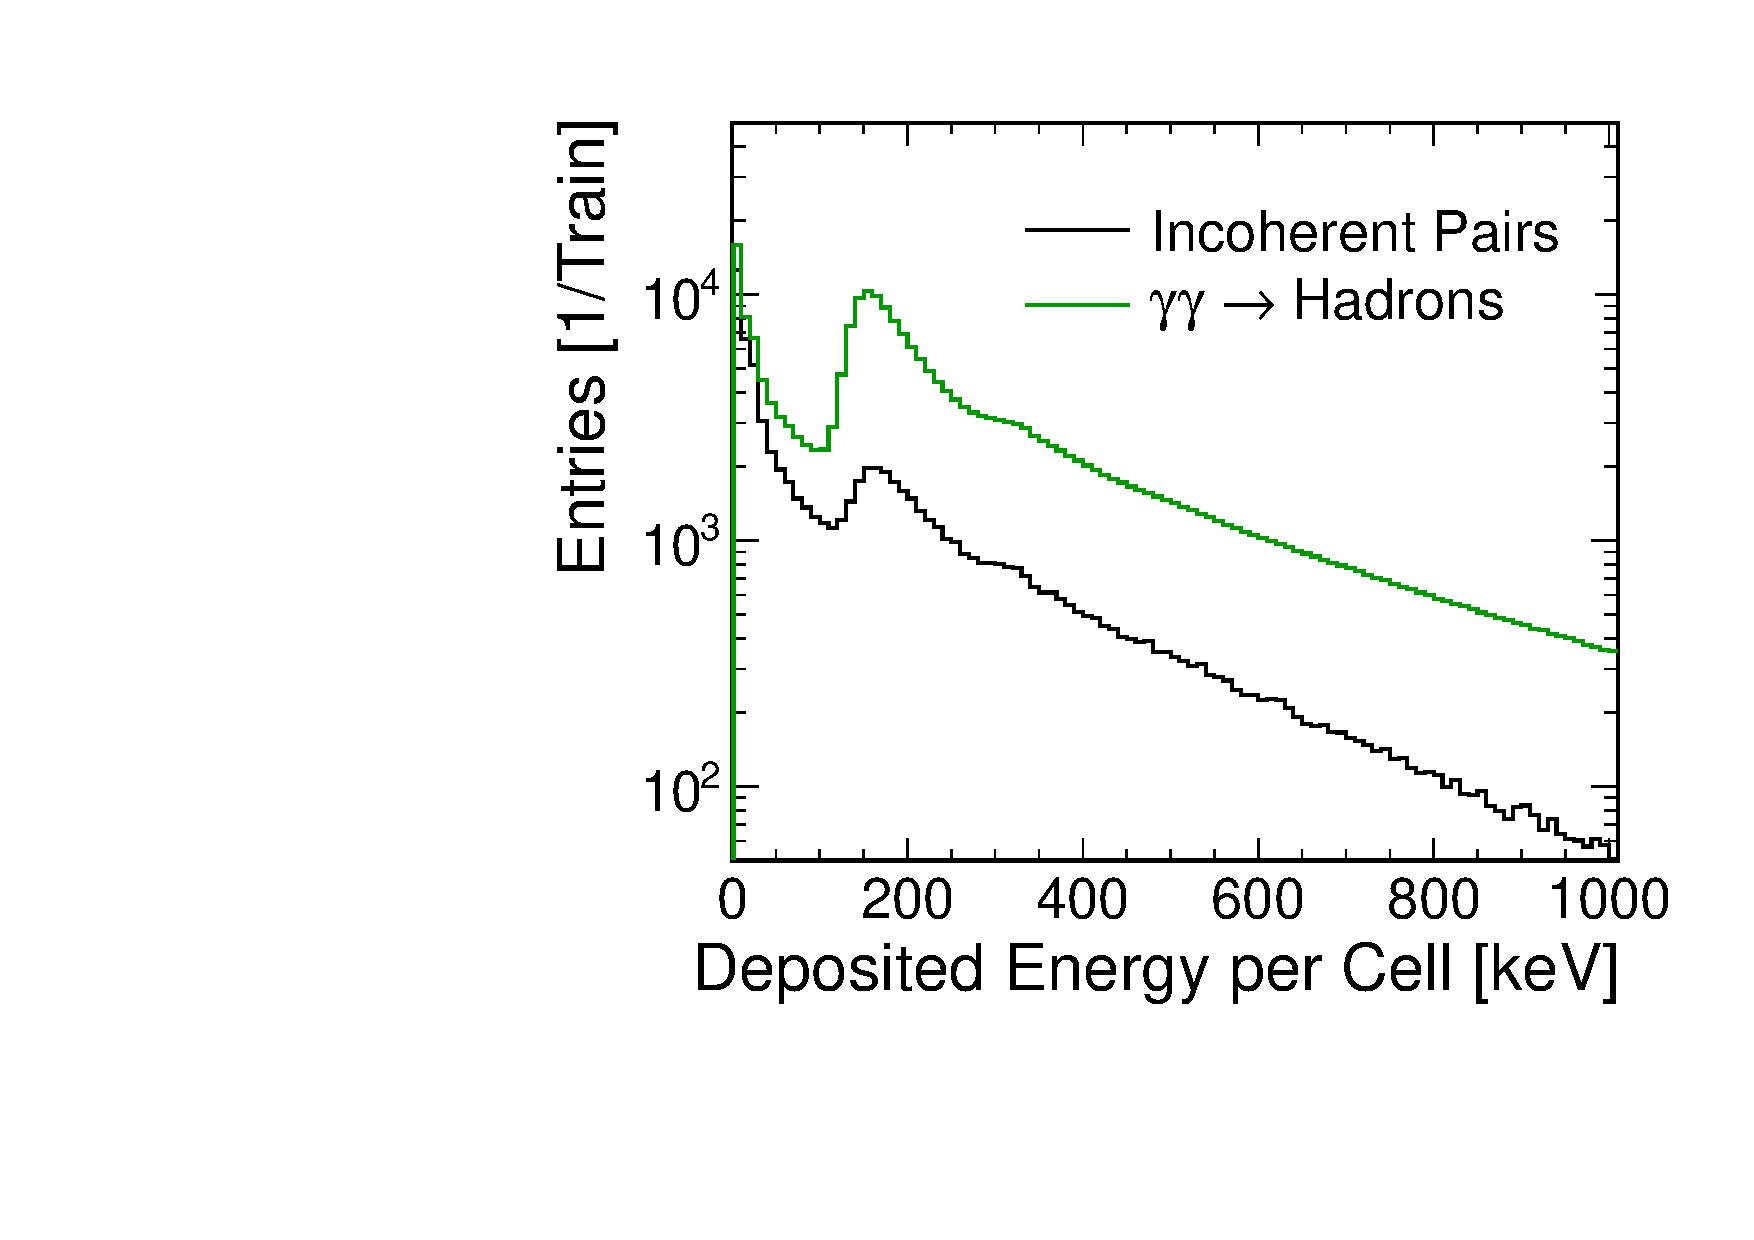
\includegraphics[width=0.49\linewidth]{../Chap3_ExpCond_PhysPerfsReqs/ECalEnergyGandPMacro.pdf}
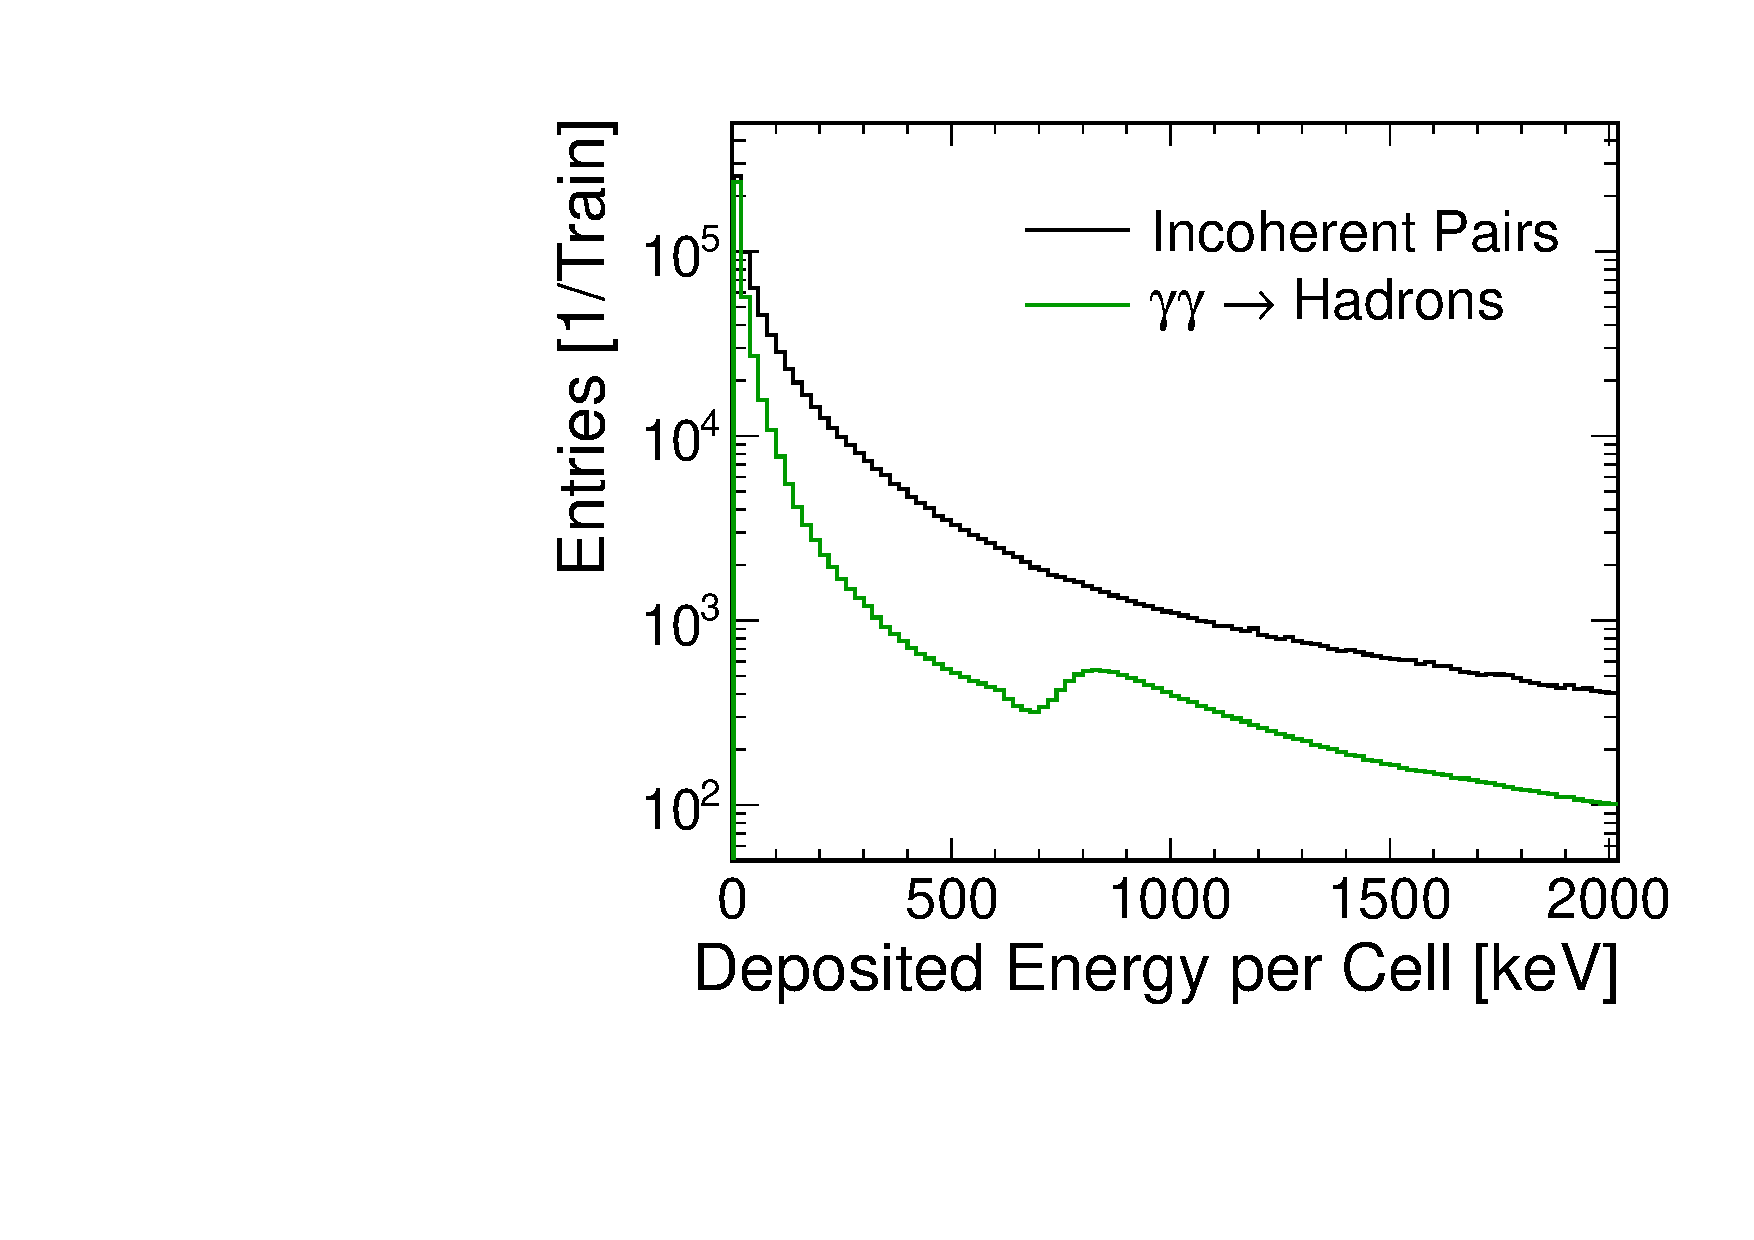
\includegraphics[width=0.49\linewidth]{../Chap3_ExpCond_PhysPerfsReqs/HCalEnergyGandPMacro.pdf}
 \caption{Distributions of the hit energies in the \clicild ECAL
   (left) and HCAL (right) endcaps for an entire bunch train of
   background. The normalisation is applied for nominal background
   rates, excluding safety factors for the simulation uncertainties.
 \label{fig:chap3:caloBackEnergy}}

\end{figure}



Figure~\ref{fig:chap3:caloBackEnergyEnergy} shows the radial distribution of the
background in the endcaps. In the ECAL, the background extends out to relatively
large radii. In the HCAL the background from \gghadrons also extends out to
large radii, but at smaller radii it is swamped by neutrons arising from the incoherent pair
background. 
\begin{figure}[hbt]
\centering
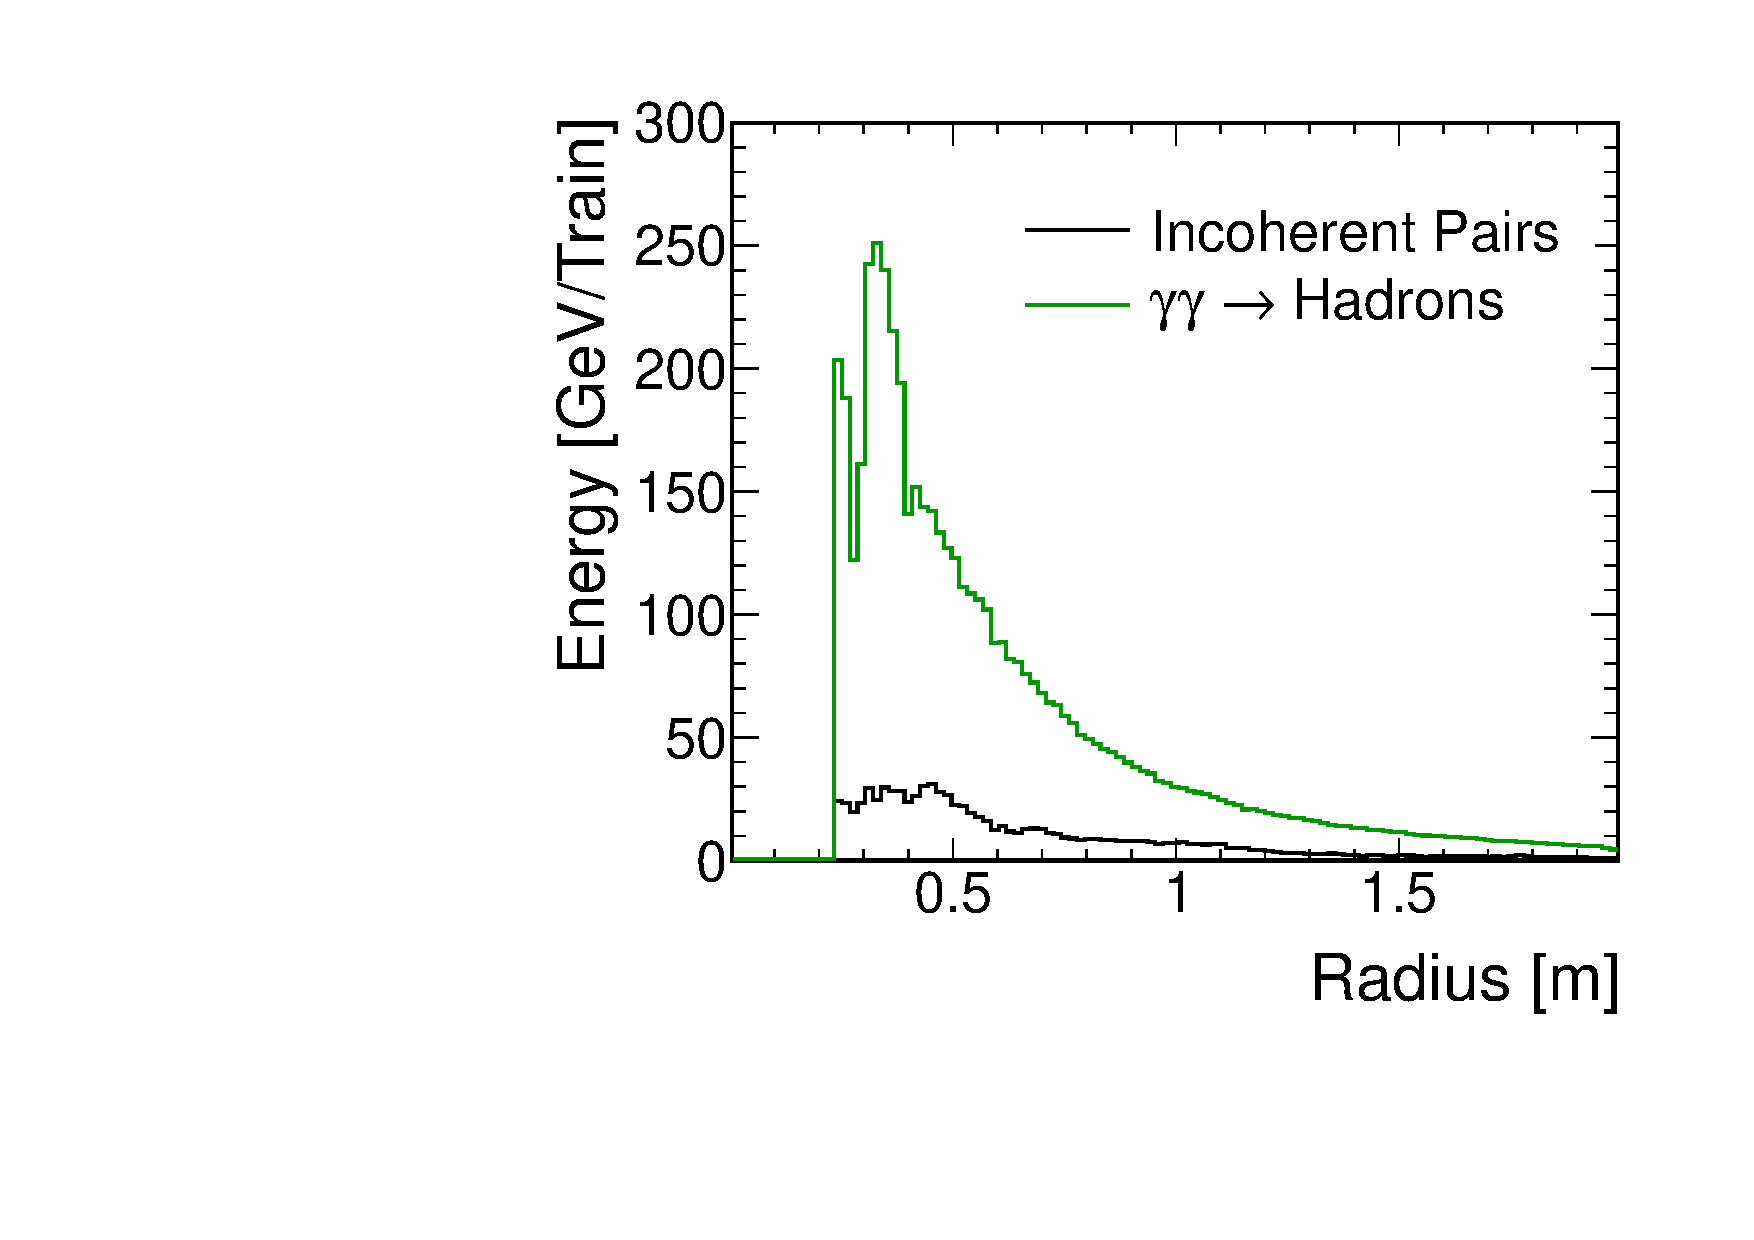
\includegraphics[width=0.49\linewidth]{../Chap3_ExpCond_PhysPerfsReqs/ECalEnergyRadiusGandPMacro.pdf}
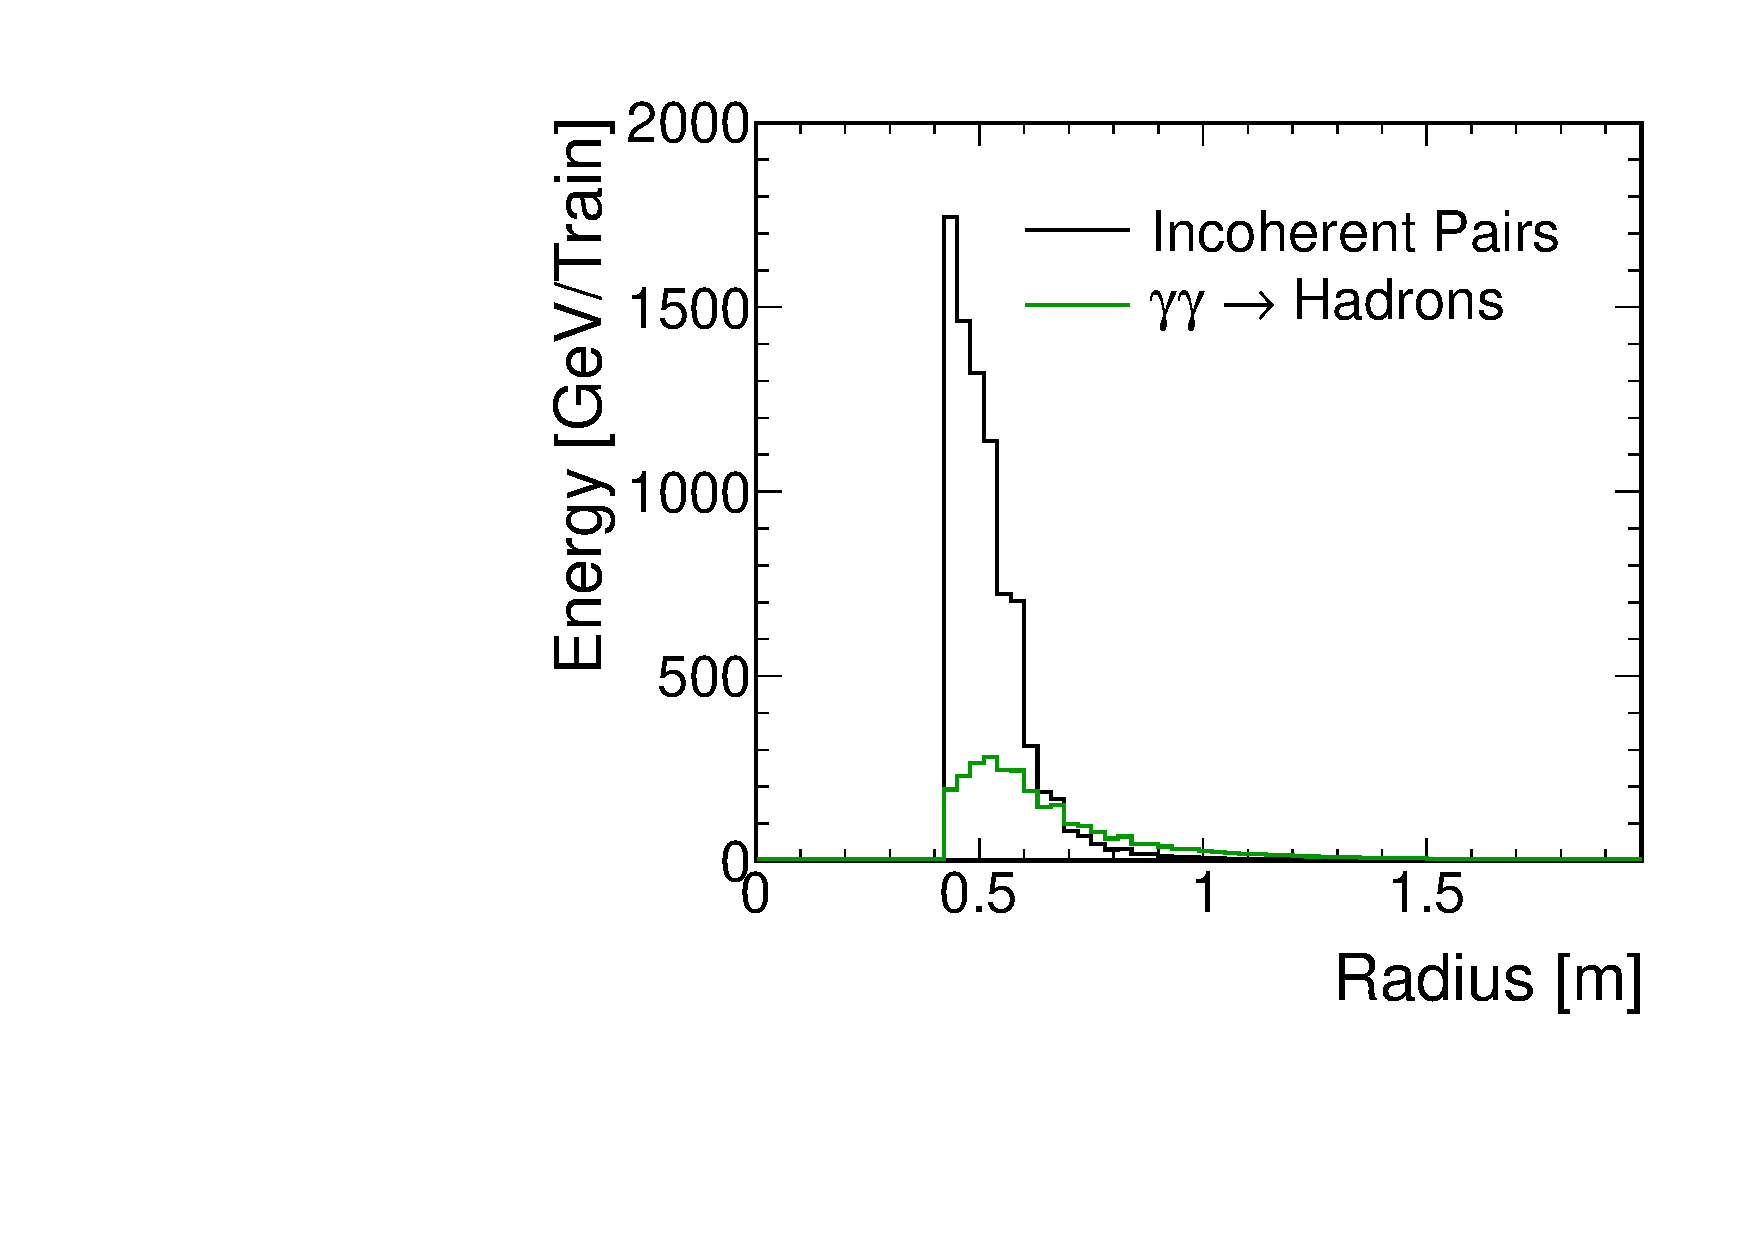
\includegraphics[width=0.49\linewidth]{../Chap3_ExpCond_PhysPerfsReqs/HCalEnergyRadiusGandPMacro.pdf}
 \caption{Radial distribution of the calorimetric energy deposition in \clicild ECAL (left) and HCAL (right) endcaps for an entire
 bunch train from within 300~ns of the start of the train. The normalisation is applied for nominal background
   rates, excluding safety factors for the simulation uncertainties.
The dip at approximately 0.3~m is due to the relatively thick
 beam pipe. The
 structure at 0.40~m in the ECAL corresponds to a small gap between calorimeter components. 
 \label{fig:chap3:caloBackEnergyEnergy}}

\end{figure}


Given that the backgrounds for an entire bunch train are high it is clear that
the calorimeter read out needs to be able to resolve multiple hits per bunch train. Another important consideration
is the level of occupancy per calorimeter cell which, in part, determines the
required two-hit time separation. Again this can only be considered in the 
context of a particular detector design and calorimeter readout cell size. In
the simulation of the \clicild detector, the Silicon sensors in the ECAL are
$5\times5~\mathrm{mm}^2$ and the scintillator tiles in the HCAL are 
$3\times3~\mathrm{cm}^2$. For the occupancy calculation the time
window of 300~ns from the start of the bunch train was divided into twelve
25~ns time windows. The mean number of hits above threshold, taken to be 0.3
minimum ionising particle equivalent, is shown for the ECAL and HCAL in
Figure~\ref{fig:chap3:caloBackOccupancy}. In the ECAL the occupancies at low
radii approach 50\% per bunch train and are dominated by the background from
\gghadrons. From Poisson statistics this implies that approximately 40\% of
cells at the inner most radii have at least one background hit per bunch train.
In order for this region of the calorimeter to be useful, the ECAL readout must
be capable of multiple-hit resolution within the bunch train. In the HCAL the
occupancies from \gghadrons are comparable to those in the ECAL reaching a
maximum of about one per train at the inner radii of the calorimeter. However,
the occupancy in the inner region of the HCAL from neutrons produced by the
incoherent pairs in the BeamCal approaches one hit per assumed 25~ns
time window. 


\begin{figure}[hbt]
\centering
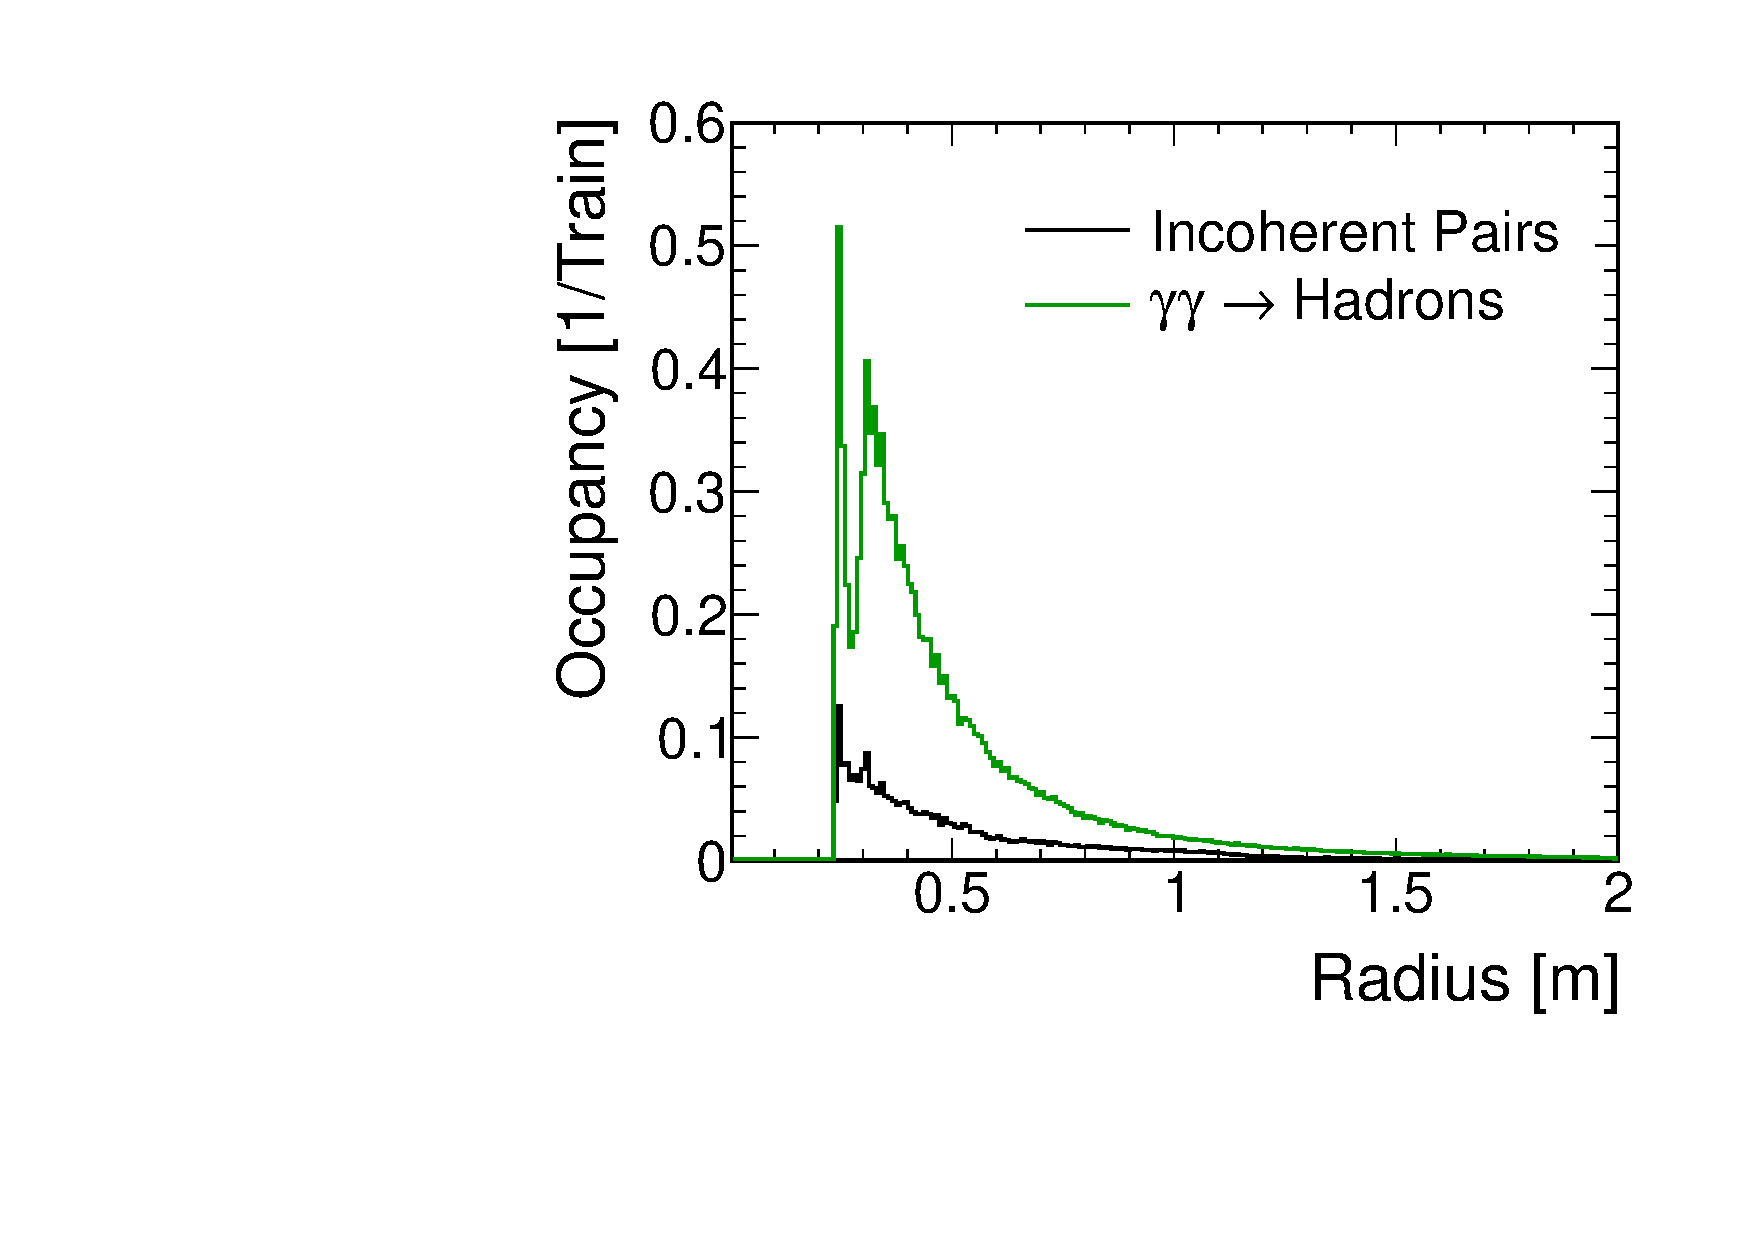
\includegraphics[width=0.49\linewidth]{../Chap3_ExpCond_PhysPerfsReqs/ECalRadiusGandPMacro.pdf}
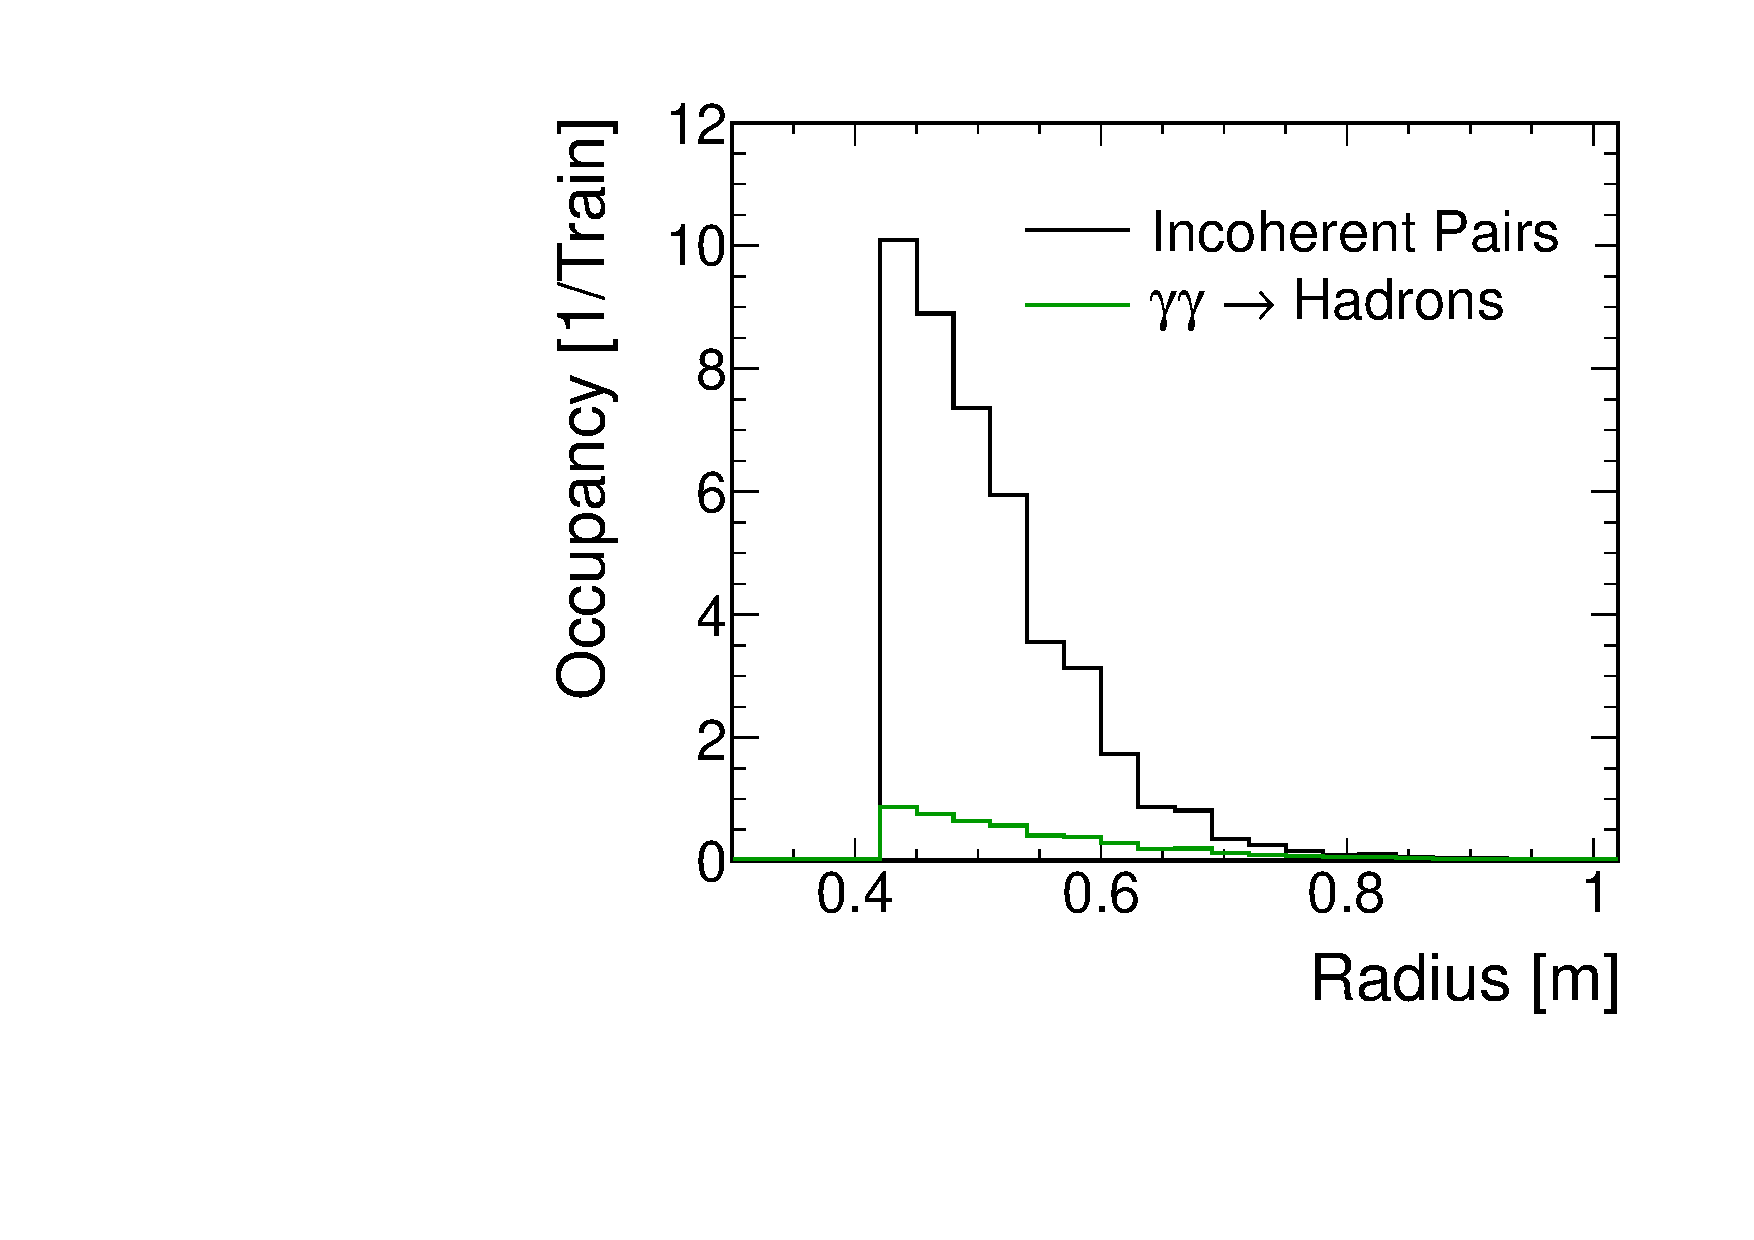
\includegraphics[width=0.49\linewidth]{../Chap3_ExpCond_PhysPerfsReqs/HCalRadiusGandPMacro.pdf}
 \caption{Average cell occupancy in the ECAL (left) and HCAL (right) endcaps of the \clicild detector. In the case of the ECAL 
 the average is given for layers 5 -- 10 which broadly correspond to maximum energy deposit of typical
 EM showers. In the case of the HCAL the average is quoted for layers 35 -- 45 where the maximum activity
 from the neutron background is observed. The results are obtained for nominal background
 rates, excluding safety factors for the simulation uncertainties.
  \label{fig:chap3:caloBackOccupancy}}

\end{figure}

The total energy deposition and associated occupancies at the inner radii of the
HCAL would pose a serious problem for event reconstruction in these regions.
However, the forward region of the \geant models of the \clicild and \clicsid
detector concepts were designed before the impact of the scattered neutron
background from the incoherent pairs interacting in the BeamCal was fully understood.
The level of background in the low radius region of the HCAL in the current
detector models is too high. However, there are a number of possible ways in which
to reduce this component of the background. These will be studied in the future and include: increased shielding
between the BeamCal and the inner regions of the HCAL; the possibility
of using a different active material which, unlike plastic scintillator, is relatively
insensitive to neutrons; and increasing the transverse segmentation to resolve
the occupancy issue. 

For the detector studies presented in Chapter~\ref{chapter_14} of this CDR, only the backgrounds from
\gghadrons are routinely included in the simulation. For all regions of the
calorimeters, with the exception of the inner part of the HCAL endcap, this is
the dominant source of background both in terms of the number of hits and the
total energy deposition. 

\subsubsection{Background Summary}

Table~\ref{tab:chap3:clicBackgrounds} summarises the simulated background conditions 
in the \clicild detector for an entire CLIC bunch train. The total calorimetric energy 
deposition of 37~TeV is large compared to the centre-of-mass energy and implies strict 
requirements on the timing resolution of CLIC calorimeters. Even excluding the HCAL contribution 
from the incoherent pair background, the overall energy deposited in the CLIC detector corresponds 
to about 20~TeV per bunch train. This is predominantly forward peaked 
(see Figure~\ref{fig:chap3:caloBackEnergyEnergy}), but nevertheless poses a serious challenge to 
the design of a detector at CLIC\@. 
\begin{table}[!htb]
\centering

  \caption{Summary of the background conditions in the \clicild detector model.
    The numbers correspond to the background for an entire CLIC bunch
    train and were obtained for nominal background rates, excluding safety
    factors for the simulation uncertainties. The
    reconstructed calorimeter energies are integrated over 300~ns from the start of
    the bunch train. The backgrounds in the HCAL from incoherent pairs are
    pessimistic as no attempts to mitigate the effect of neutrons from incoherent
    pair interactions in the \acs{BeamCal} have been made.
    \label{tab:chap3:clicBackgrounds}}
  \begin{tabular}{l c c }
    \toprule
    Subdetector       & Incoherent Pairs & \gghadrons   \\  
                      & \tabt{[TeV]}     & \tabt{[TeV]} \\ \midrule
    ECAL Endcaps      & 2                & 11           \\ 
    ECAL Barrel       & --               & 1.5          \\
    HCAL Endcaps      & 16               & 6            \\      
    HCAL Barrel       & --               & 0.3          \\ \midrule
    Total Calorimeter & 18               & 19           \\ \midrule
    Central Tracker   & --               & 7          \\ \bottomrule
  \end{tabular}
\end{table}

\section{Timing Requirements at CLIC\label{sec:chapter3:clic_detector:timingRequirements}}

The backgrounds presented in Table~\ref{tab:chap3:clicBackgrounds} are for the
full train of 312 bunches separated by 0.5~ns. The most obvious way to reduce
the backgrounds associated with a particular physics event is to time stamp the
hits from the detector and impose tight timing cuts. The background from
\gghadrons is proportional to the number of bunch crossings which are
superimposed on the physics interaction. This is determined by the subdetector
time integration windows and thus the requirements are driven by the impact of
the background on reconstructed physics observables. Whilst the \gghadrons
background is high, the majority of the particles have low values of
\pT as shown in Figure~\ref{fig:chap3:gghad-pt} and any tight timing cuts can be restricted to
relatively low \pT particles. 

The timing requirements at CLIC are driven by the levels to which the background
degrades the physics performance of the detector. Provided the occupancies in
the elements of the tracking detectors are sufficiently low that efficient
track reconstruction is possible, there is unlikely to be a significant impact
on the quality of the reconstructed tracks. Hence the main impact of the
background will be on the reconstruction of jets. As an example
Figure~\ref{fig:chap3:wwReco} shows a generator level study of the \PW-boson mass
resolution for simulated $\PW \rightarrow \mathrm{qq}$ decays, where the energy
of the \PW-boson is 500~GeV, with different numbers of bunch crossings of
\gghadrons background superimposed. The jet energy resolution is assumed to be
3.5\%. Only particles above a \pT cut are used in the jet finding to suppress
the effects of the \gghadrons background. 
The impact of the background on the reconstructed mass
distribution is significant. The reconstructed width increases by approximately
70\% when 20~BXs (10~ns) of background are overlaid, equivalent to a factor
three reduction in effective luminosity. 
Figure~\ref{fig:chap3:wwReco}  also shows
the reconstruction of a high mass di-jet state as a function of the assumed level of
background, in this case the reconstructed heavy Higgs mass from the process $\epem\rightarrow\PHz\PSAz\rightarrow \bbbb$.
From these and other studies it is
concluded that the acceptable level of background should correspond to 5--10~BXs, requiring a time resolution of
$<5$~ns. It should be noted that, in reality, simple \pT cuts will be less effective than shown here due to 
pile-up from multiple background particles faking higher \pT photons and neutral hadrons, thus the plots in 
Figure~\ref{fig:chap3:wwReco} underestimate the impact of the background.
\begin{figure}[hbt]
\centering
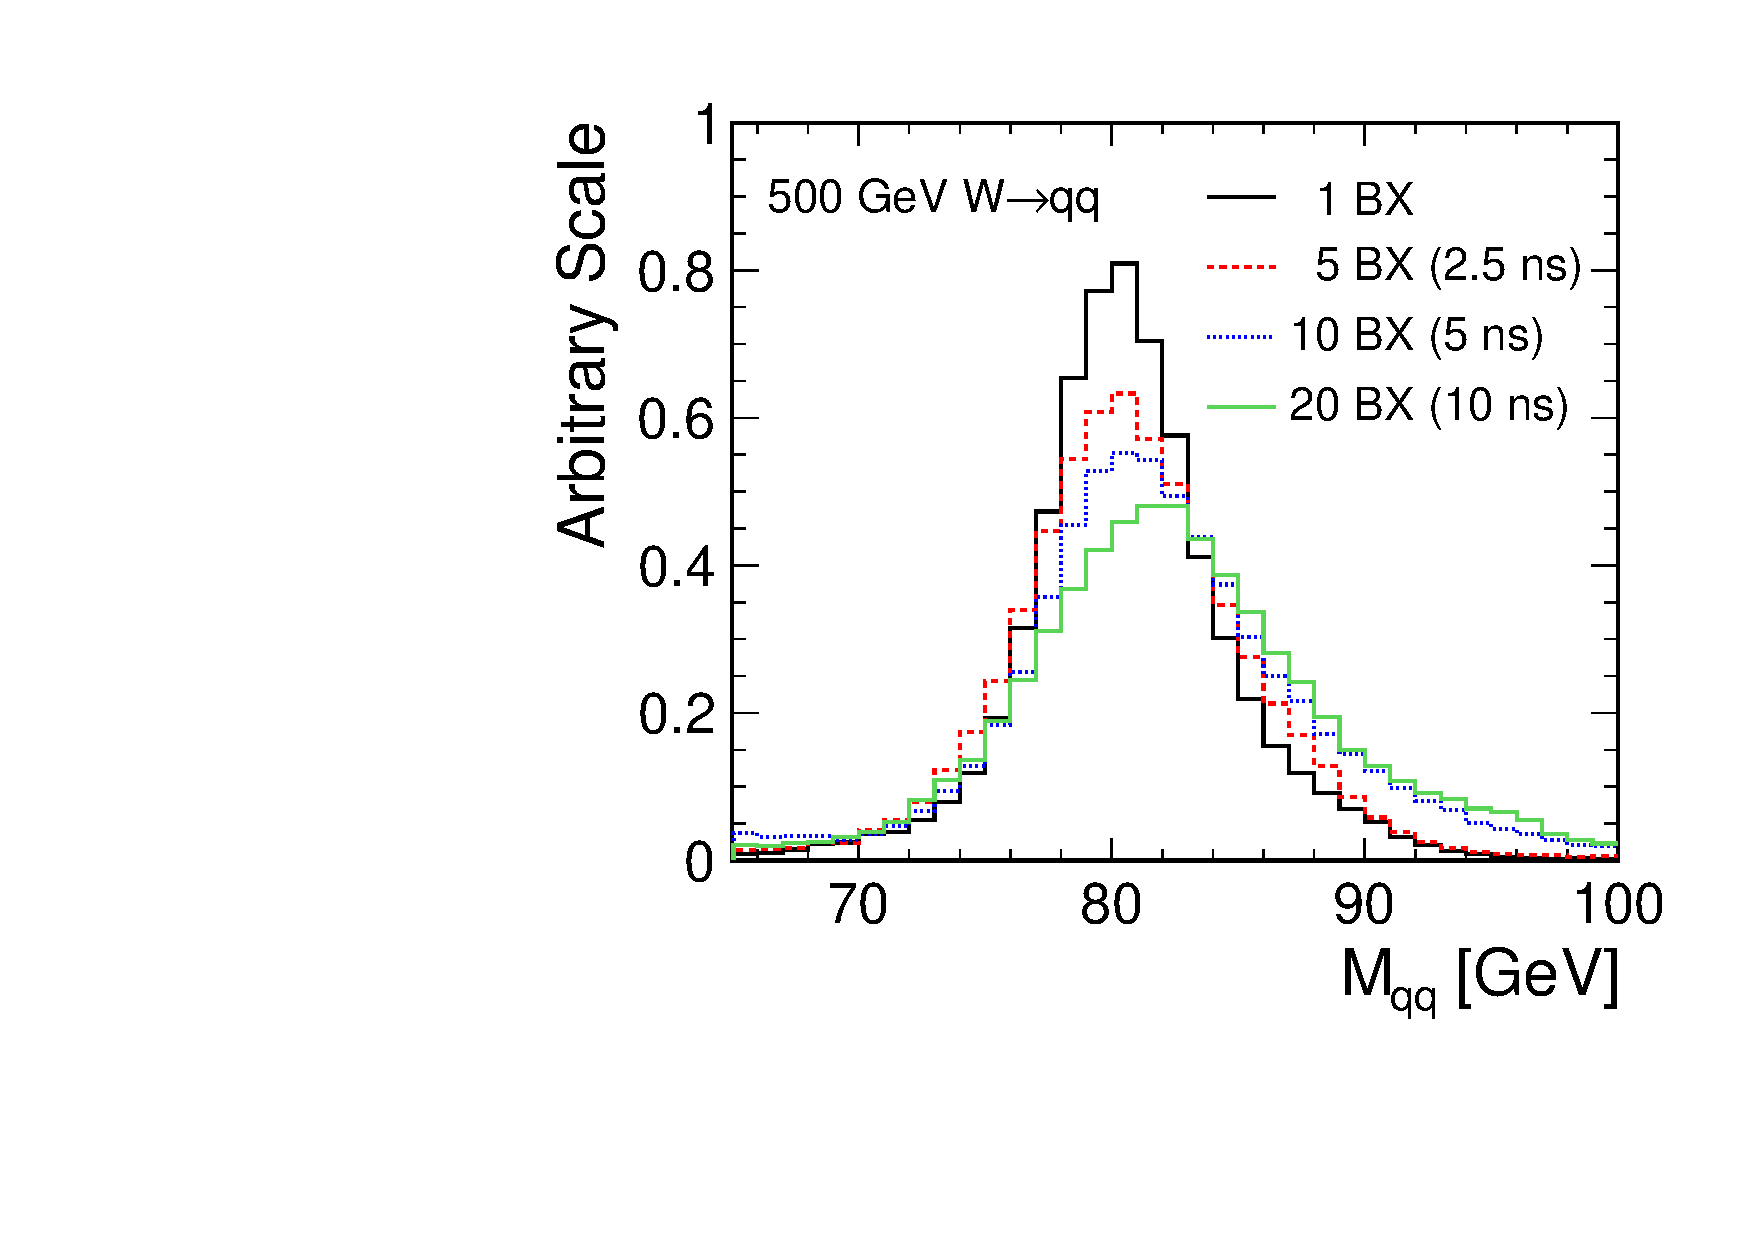
\includegraphics[width=0.49\linewidth]{../Chap3_ExpCond_PhysPerfsReqs/WTiming.pdf}
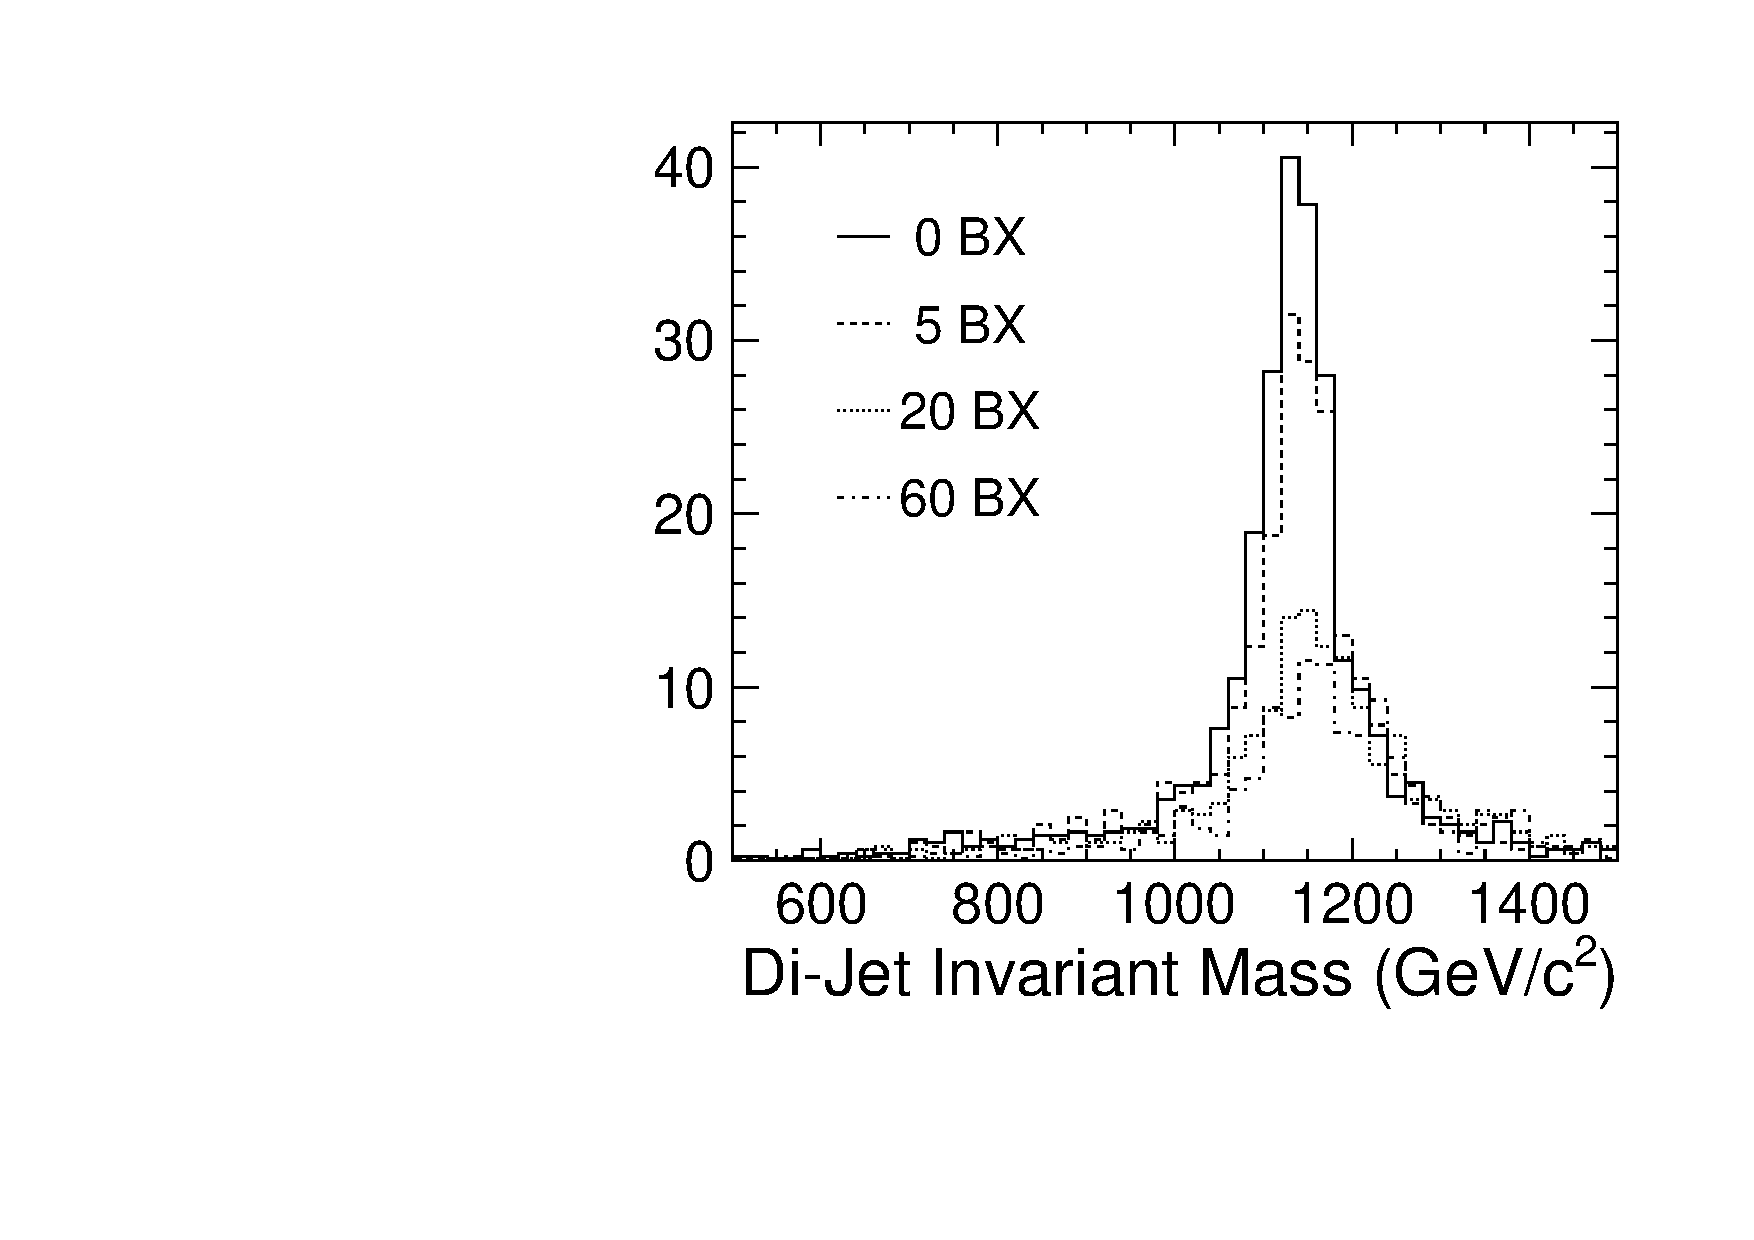
\includegraphics[width=0.49\linewidth]{../Chap3_ExpCond_PhysPerfsReqs/habx.pdf}
 \caption{(left) Reconstructed \PW boson mass distribution as a function
   of the assumed number of bunch crossing of background superimposed on 
   500~GeV $\PW\rightarrow \mathrm{qq}$ decays. Jets are reconstructed as using the \kT-algorithm,
   discussed in Chapter~\ref{chapter_14}, with a cut on $\Delta R = 0.7$. In each case, a \pT cut is applied. The
    cut value depends on the number
    of bunch crossings of background overlaid and ranges from 0.5~GeV for 5~BXs to
    1.0~GeV for 20~BXs.   (right)  Reconstructed heavy Higgs mass in the process $\epem\rightarrow\PHz\PSAz\rightarrow \bbbb$
     for different levels of assumed background. In each case a \pT cut of 0.9~GeV is applied.
     \label{fig:chap3:wwReco}}
\end{figure}

From the above arguments it might be concluded that a 5\,ns time-stamping capability is required for all
subdetectors. However, regardless of the practical considerations, there is a fundamental limitation to
the minimum time window from which it is viable to read out the calorimeters;
because the propagation speed of the particles in hadronic showers is finite and
the energy released in nuclear processes is not instantaneous on the timescale
of 1~ns. Consequently a finite time window is required to accumulate the
majority of the energy depositions associated with a hadronic shower. This has
been studied in a \geant simulation of the \clicild calorimeters using the
high precision \qgspberthp physics list. Calorimeter hit times are corrected
for straight-line time-of-flight from the \acs{IP}. Figure~\ref{fig:chap3:caloTiming}
shows the cumulative fraction of the total energy as a function of time for
steel and tungsten absorbers. For the HCAL endcap with steel for the absorber
material 90\% of the energy is recorded within 6~ns (corrected for
time-of-flight). For the tungsten absorber assumed for the HCAL barrel, only
82\% of the energy is deposited within 25~ns. The calorimetric response of
tungsten is slower than that of steel due to the much larger component of the
energy in nuclear fragments. 
\begin{figure}[hbt]
\centering
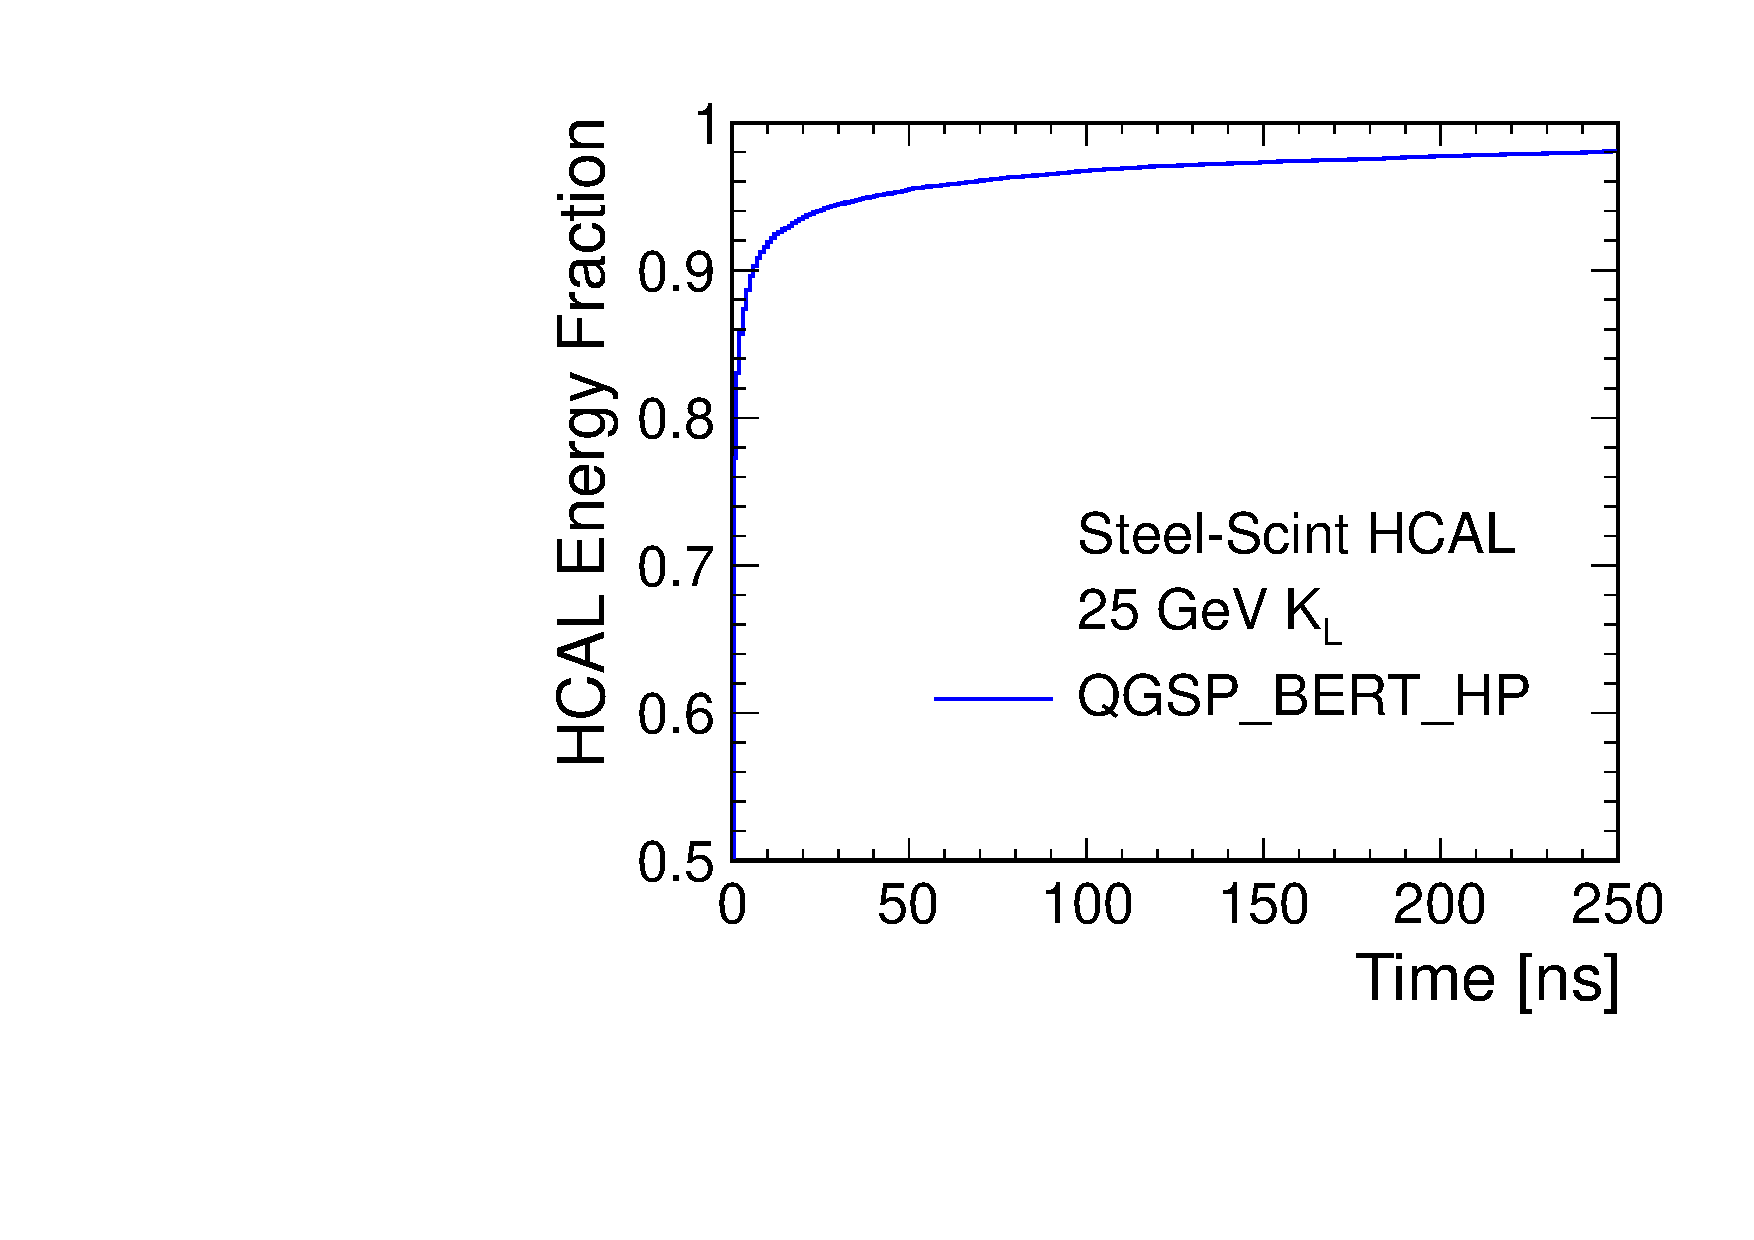
\includegraphics[width=0.49\linewidth]{../Chap3_ExpCond_PhysPerfsReqs/hcalTimingSteel.pdf}
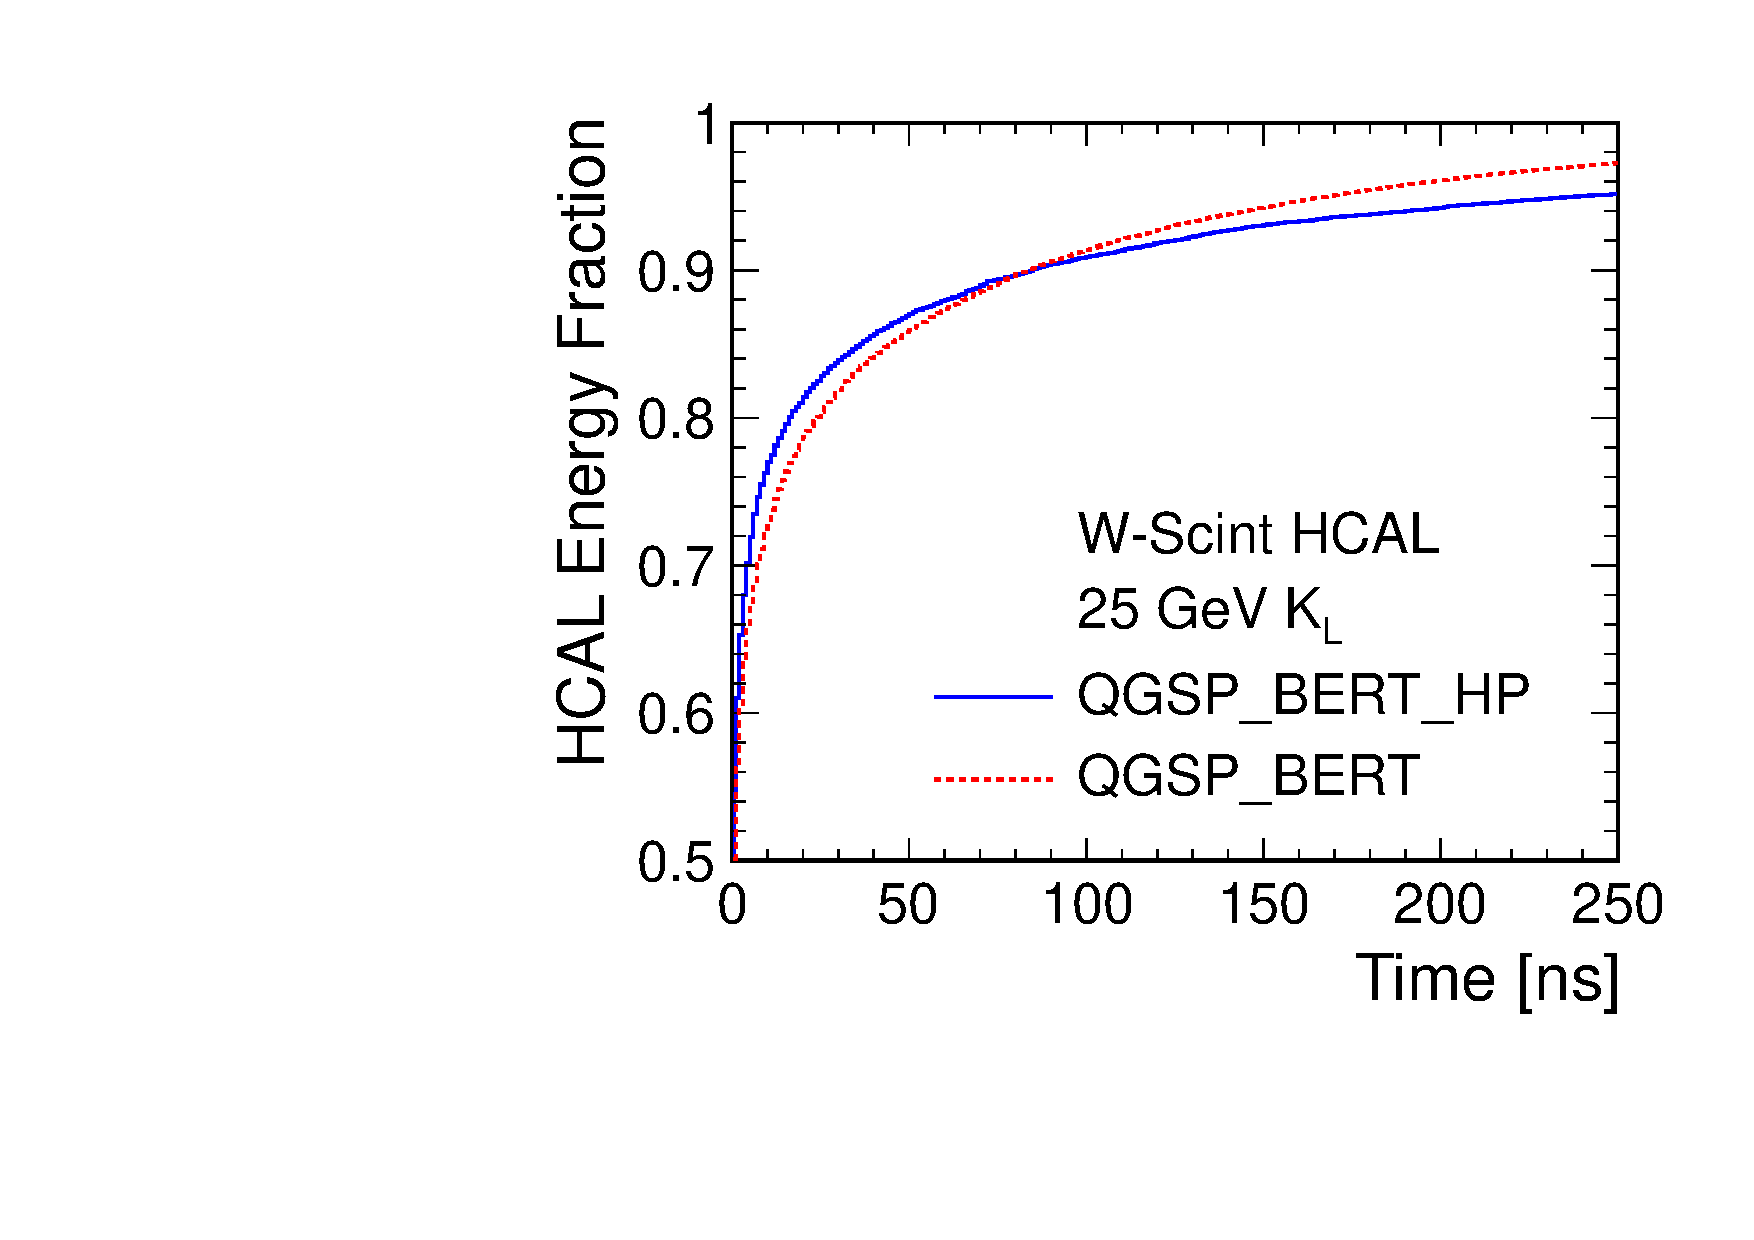
\includegraphics[width=0.49\linewidth]{../Chap3_ExpCond_PhysPerfsReqs/hcalTimingTungsten.pdf}
\caption{Fraction of total calorimetric energy recorded as a function of time
  for 25~GeV neutral hadrons as a function in the \clicild detector (left) for
  steel and (right) for tungsten HCAL absorbers. The results are based on \geant
  with the \qgspberthp physics list. Hit times are corrected for the
  straight-line time-of-flight prior to the cut. In the case of tungsten the
  plots are also shown for \qgspbert. \label{fig:chap3:caloTiming}}
\end{figure}

There is a tension between the desire for a short readout window to suppress background
and the need to read out the majority of the calorimeter hits associated with
the hard interaction. In the studies presented in this document a reconstruction
strategy has been adopted that balances these two requirements. It is this strategy,
which takes advantage of particle flow reconstruction and the highly granular
detectors being considered here, that drives the timing requirements for the CLIC detector.

\subsection{Timing in Physics Reconstruction at CLIC\label{sec:chapter3:clic_detector:physicsReconstruction}}

It is assumed that the entire bunch train of data are available for offline
reconstruction. Candidates for a hard interaction would be identified within the
bunch train and the data in a window around this time would be passed to the
event reconstruction. This integration time and the assumed single hit
resolutions for the various subdetectors are listed in
Table~\ref{tab:chap3:timingcuts}. The time window for the reconstruction in the 
calorimeters is driven by the shower development time. The single hit time
resolution of 1~ns in the calorimeters allows tighter timing cuts to be
applied to reconstructed clusters to further reduce the impact of background.
The timing requirements in the Silicon tracking detectors can be looser than the
maximum of 10~BXs suggested by studies such as those shown in
Figure~\ref{fig:chap3:wwReco}, because low momentum background tracks can be
rejected using the times of associated calorimeter clusters. An integration time
of 20~BXs is chosen, motivated by the need to reduce the combinatorics in the
track reconstruction and by the fact that not all tracks will have an associated
cluster giving a more precise time stamp. A \acs{TPC} is assumed to integrate over
the entire bunch train. All data in these time windows are passed to the track
and \acs{PFA} reconstruction software giving the reconstructed particle flow
objects (charged hadrons, photons, neutral hadrons, electrons and muons). 
\begin{table}[!htb]
\centering

  \caption{Assumed time windows used for the event reconstruction and the required single hit time resolutions.
    \label{tab:chap3:timingcuts}}
  \begin{tabular}{l c c }
    \toprule
    Subdetector         & Reconstruction window     & hit resolution   \\ \midrule
    ECAL                    & 10~ns                       & 1~ns           \\ 
    HCAL Endcaps   & 10~ns                       & 1~ns           \\      
    HCAL Barrel        & 100~ns                     & 1~ns          \\
    Silicon Detectors & 10~ns                       & 10/$\sqrt{12}$~ns   \\
    TPC                        &  entire bunch train  & n/a            \\ \bottomrule
  \end{tabular}
\end{table}

With the above timing assumptions, it is essential to demonstrate the capability of the CLIC detector concepts to
reconstruct physics events in the presence of the background from \gghadrons. For this reason, all the physics 
studies presented in this report use full \geant simulations of the CLIC detector concepts,
including background from \gghadrons overlaid on the physics events. Full track and particle flow reconstruction 
starting from the digitised hits in the time windows given in Table~\ref{tab:chap3:timingcuts} is performed.
Monte Carlo information is used at no stage in the reconstruction. Figure~\ref{fig:chap3:eventDisplays} shows the 
reconstructed particle flow objects for a simulated 
$\epem\rightarrow\PSHp\PSHm\rightarrow \tbtb$ 
event at $\roots=3$~TeV. At the reconstruction level, the background from \gghadrons produces an average energy 
of approximately 1.2~TeV per event, mostly in the form of relatively low \pT particles at relatively 
low angles to the beam axis. 
The level of \gghadrons background is roughly 1/15 of that for the entire bunch train 
(Table~\ref{tab:chap3:clicBackgrounds}), commensurate with integrating over 10~ns from the total 156~ns. 
The background can be further reduced by applying tighter timing cuts based on the reconstructed calorimeter 
cluster time. The cluster time is obtained from a truncated mean of the energy-weighted hit times constituting the cluster. In a fine grained 
particle flow detector many hits contribute to a single cluster and {\it cluster} time resolutions of <1~ns are easily
achievable. 
Efficient background rejection is achieved by using tight cuts in the range of 1.0--2.5~ns on the 
clusters (depending on the type of reconstructed 
particle and its \pT). This procedure is applied to both neutral particle flow objects and to charged objects where the 
time of the cluster associated to the track, corrected by the helical propagation time, is used. These additional timing 
cuts are applied to only relatively low \pT particle flow objects. The details of the cuts
used are discussed in 
Section~\ref{sec:chap14_backgroundOverlay}. As a result of the cluster-based timing cuts
the average 
background level can be reduced to approximately 100~GeV with negligible impact on the underlying hard 
interaction. The use of hadron-collider inspired jet-finding algorithms further reduces the impact of the background 
of \gghadrons and precision physics measurements are achievable in the CLIC background environment as 
shown in Chapter~\ref{chapter_14}.

\begin{figure}[hbt]
\centering
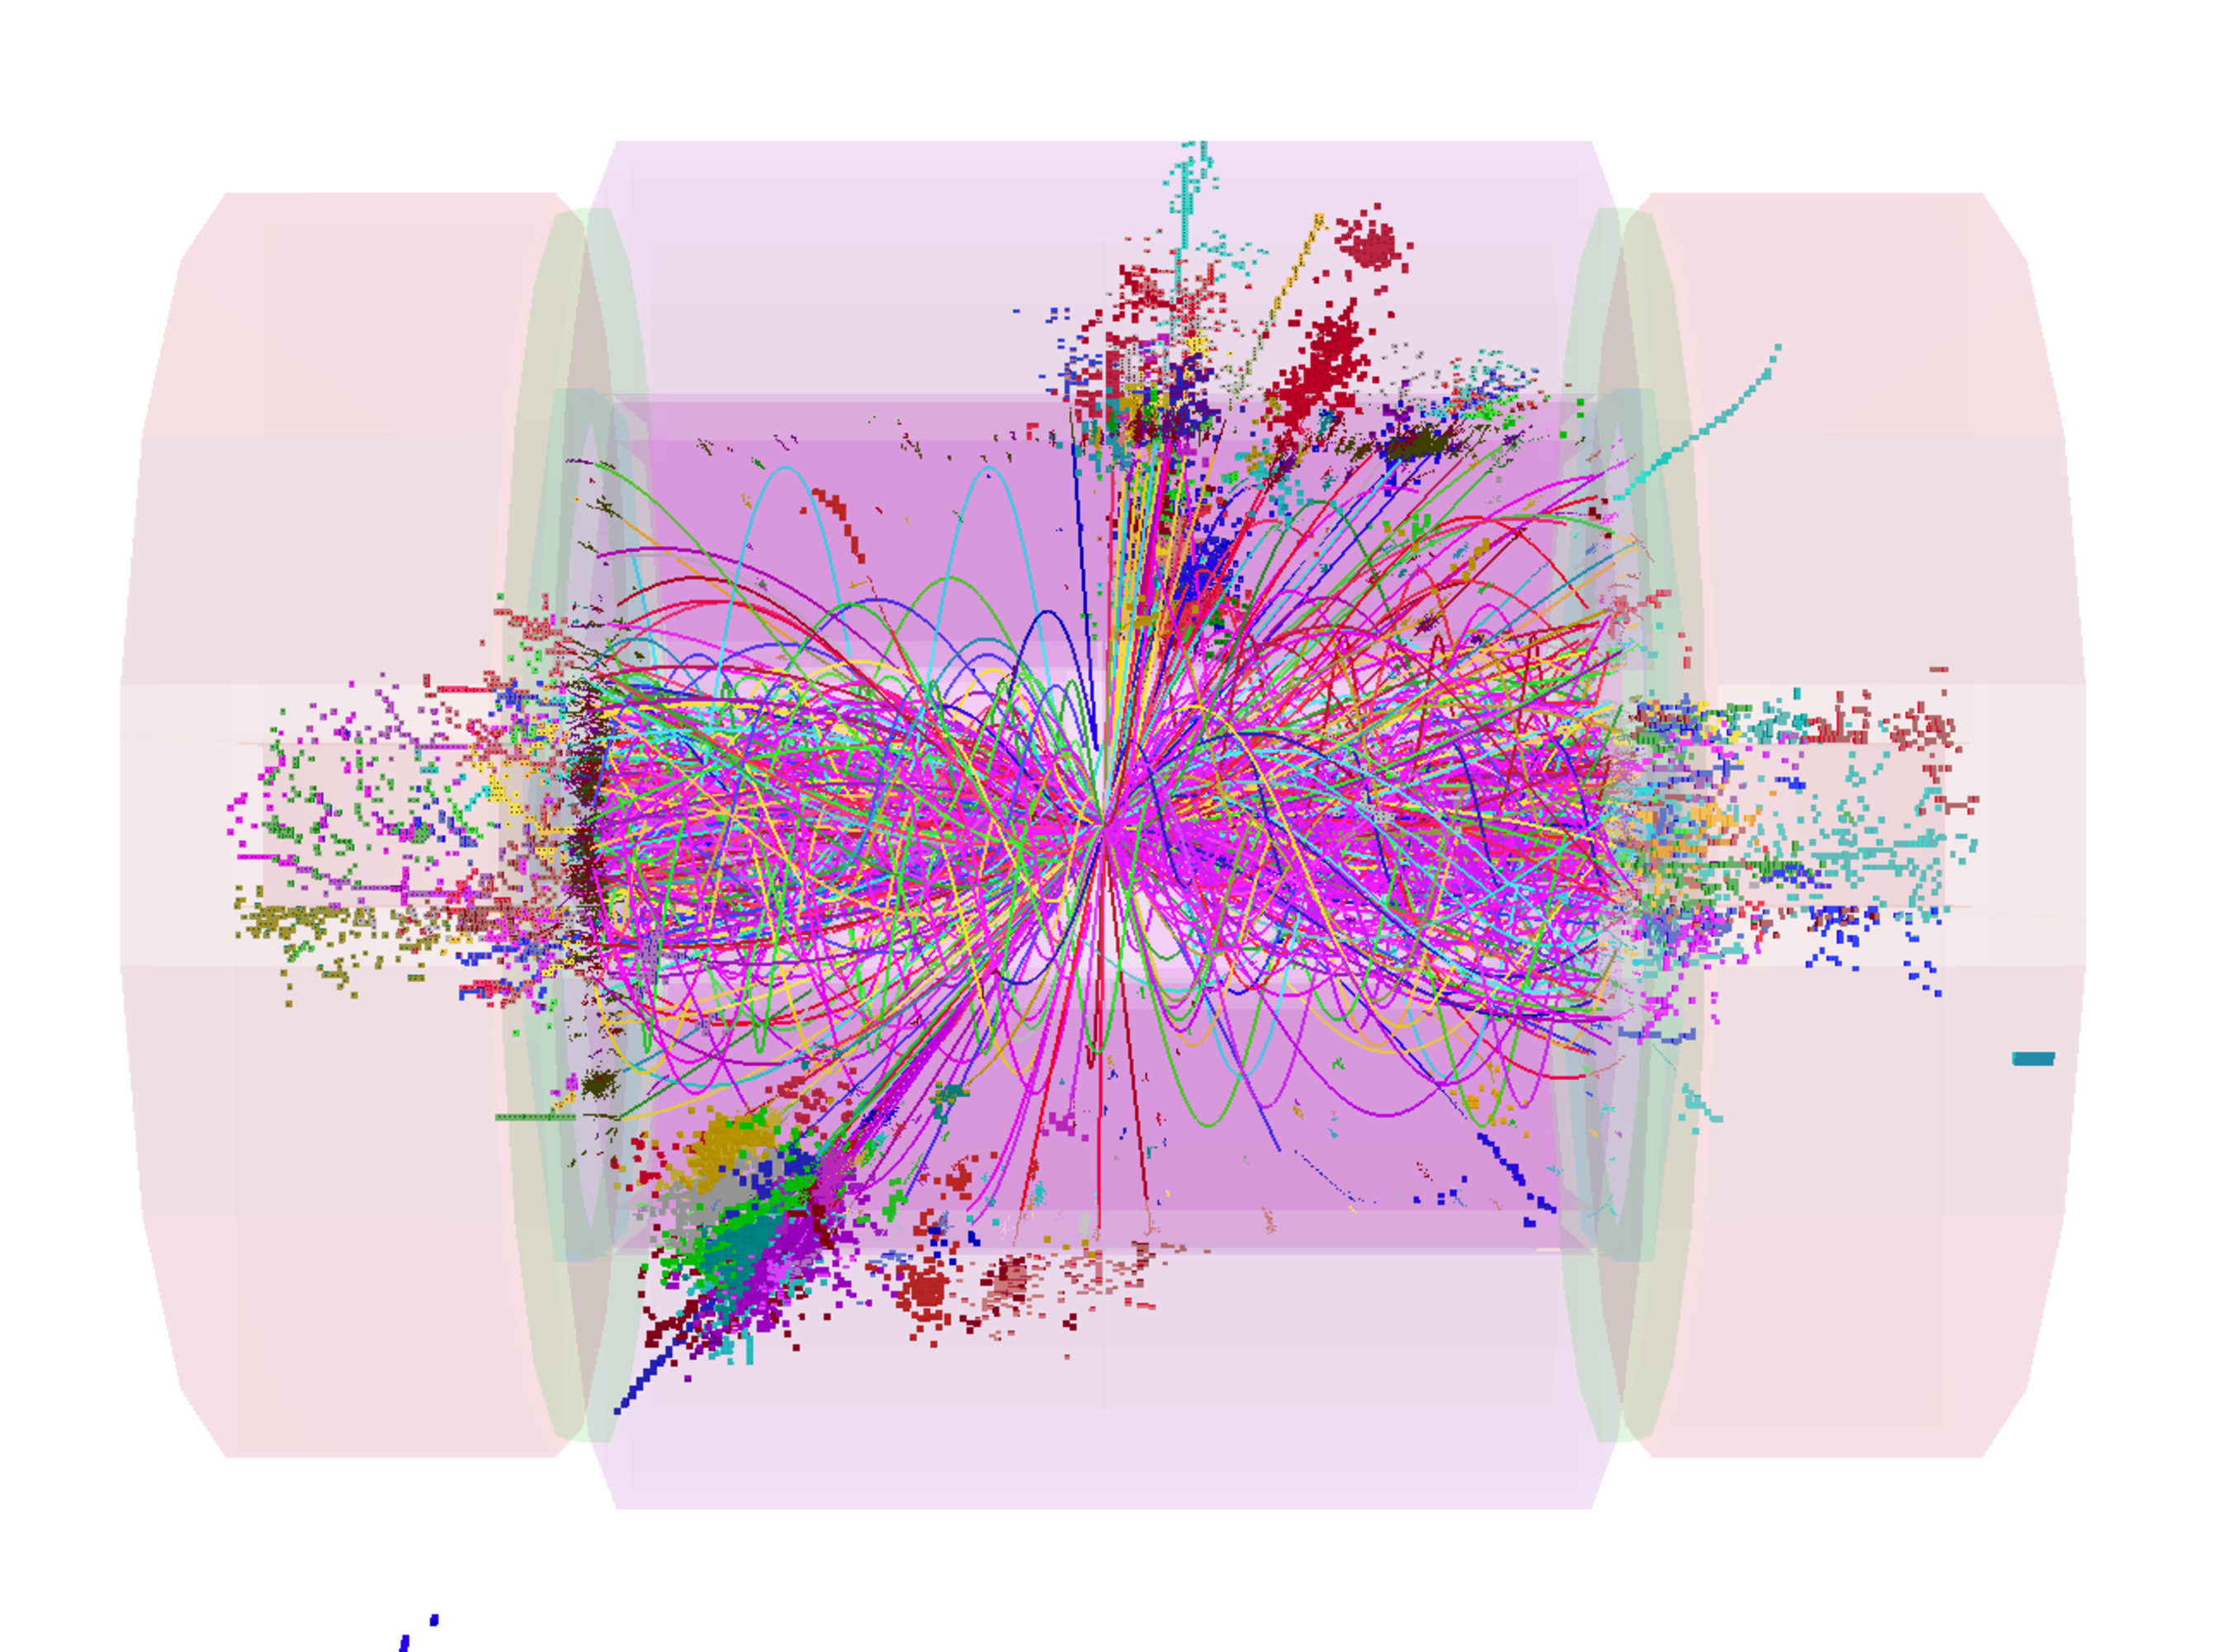
\includegraphics[width=0.49\linewidth]{../Chap3_ExpCond_PhysPerfsReqs/HH2.pdf}
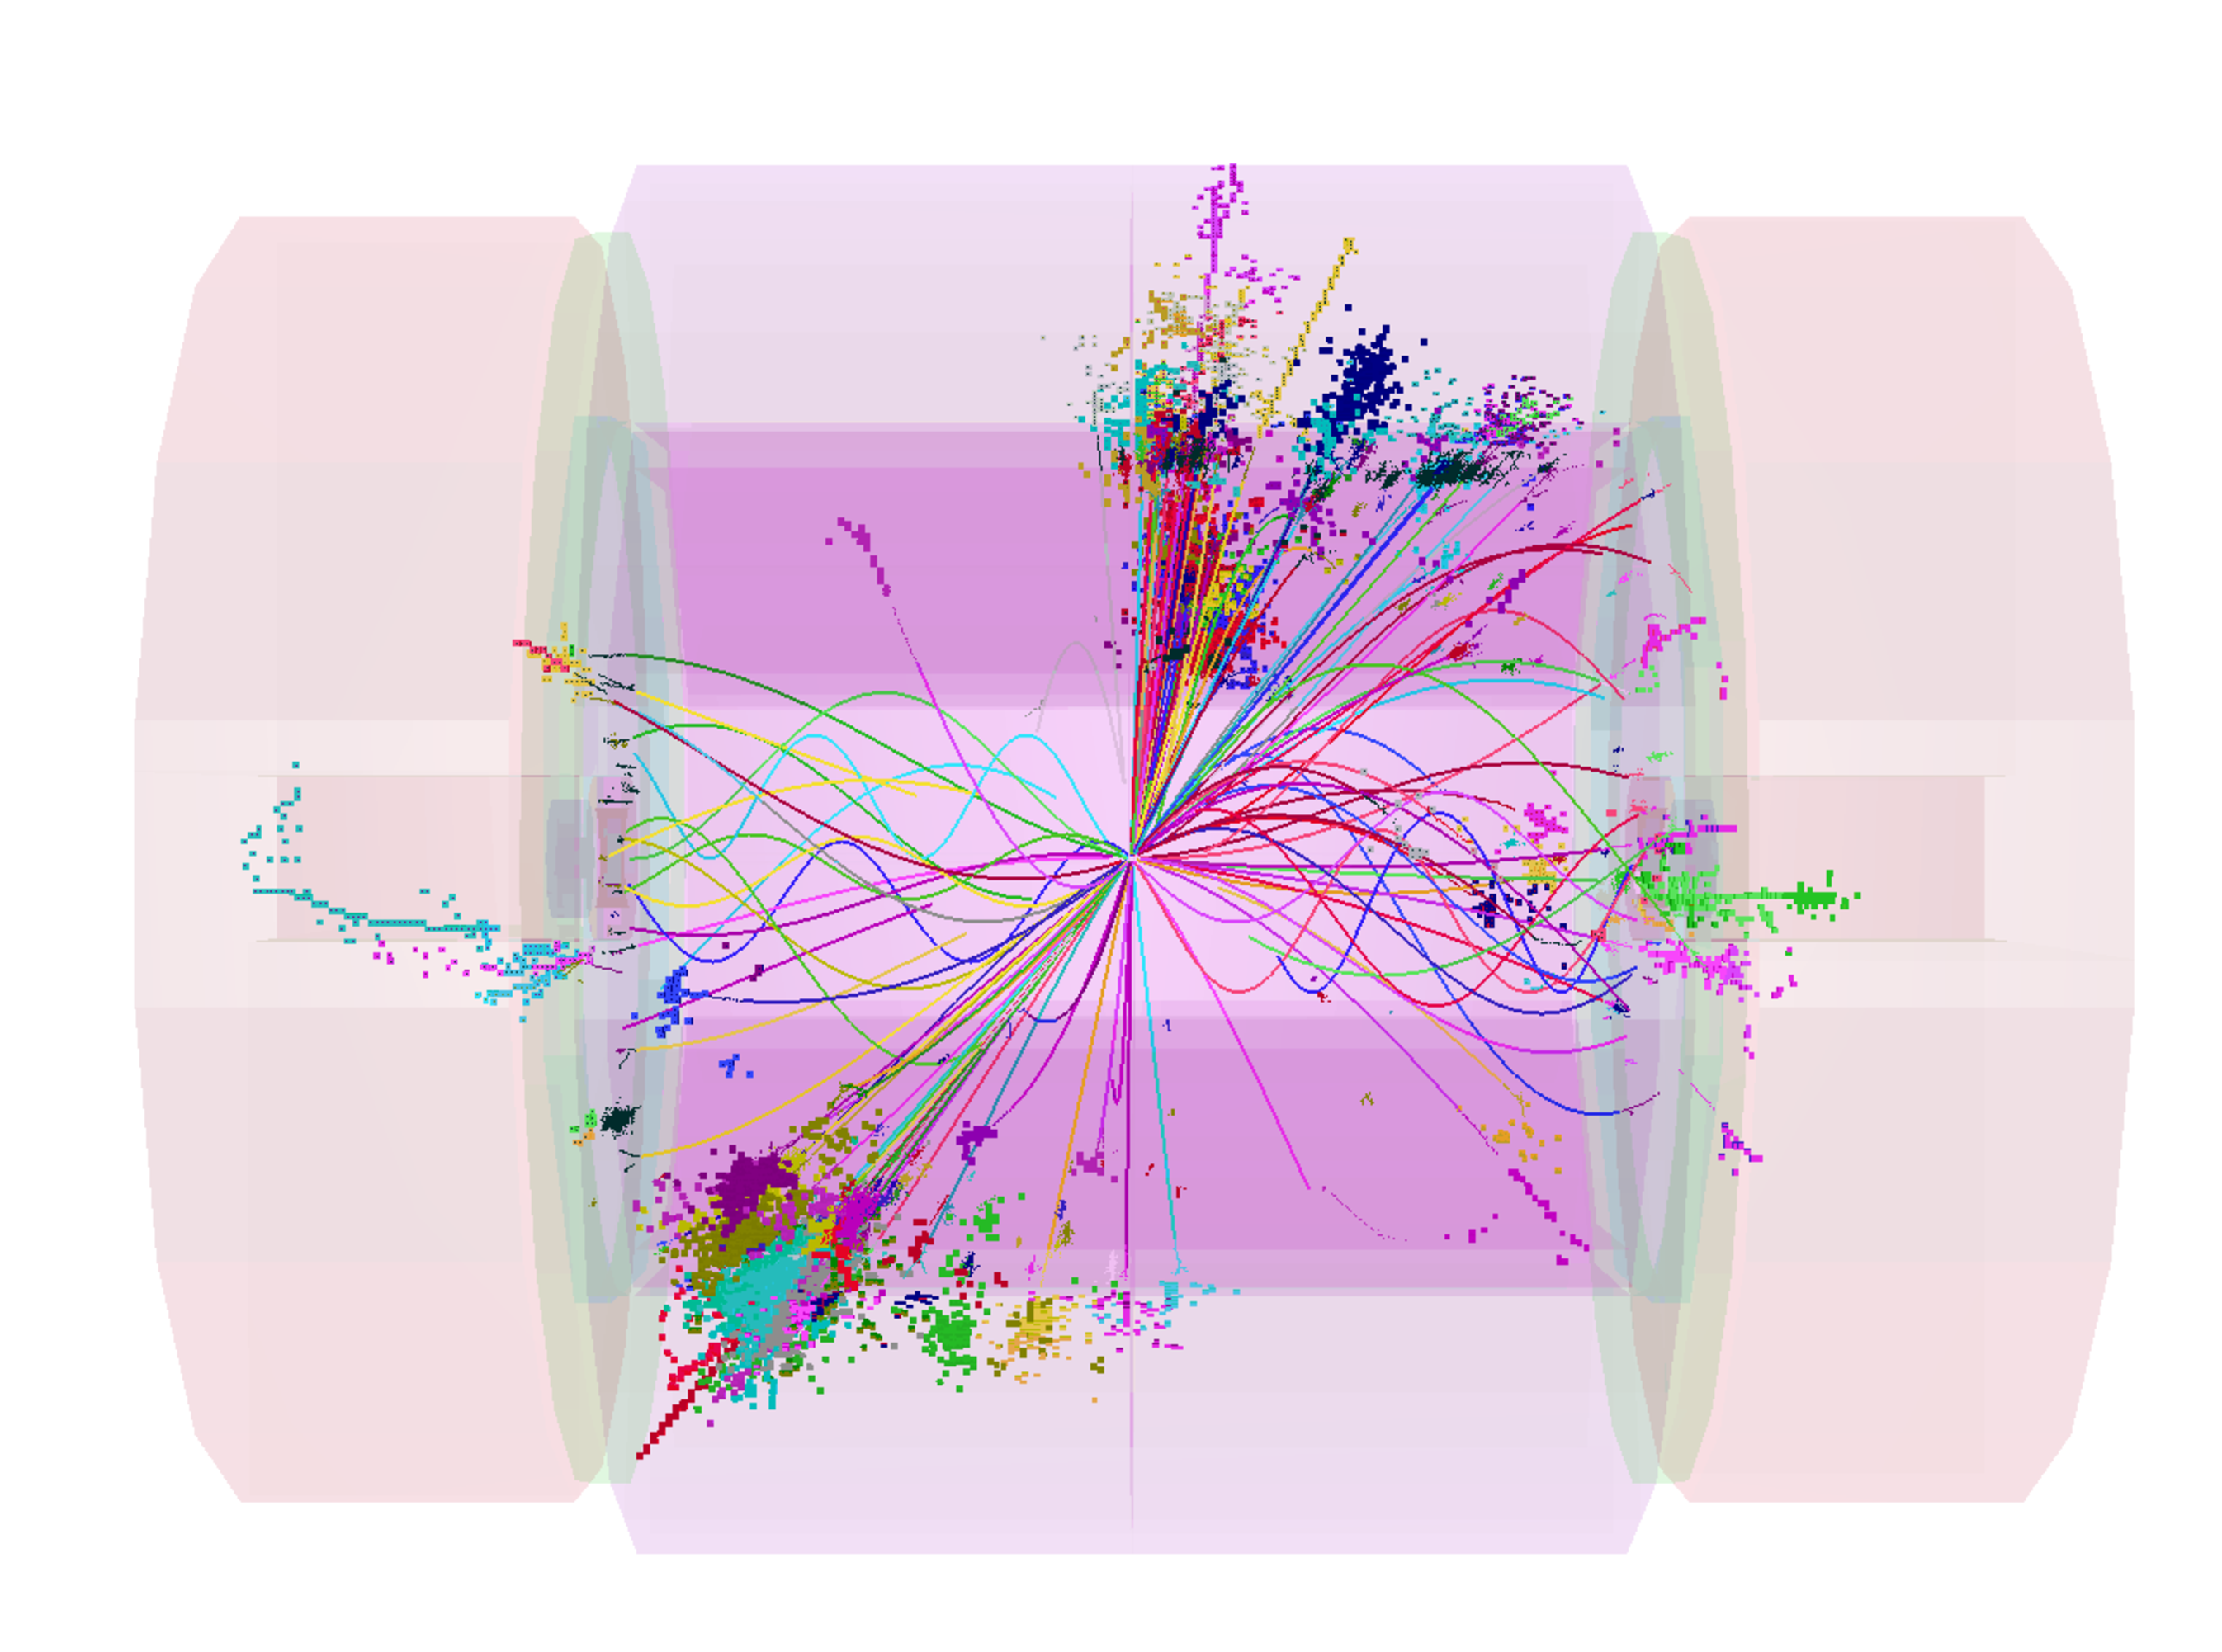
\includegraphics[width=0.49\linewidth]{../Chap3_ExpCond_PhysPerfsReqs/HH2tight.pdf}
\caption{(left) Reconstructed particles in a simulated $\epem\rightarrow\PSHp\PSHm\rightarrow \tbtb$ event at 3~TeV in the \clicild detector concept with background from \gghadrons overlaid. (right) the effect of applying tight timing cuts on the reconstructed cluster times. \label{fig:chap3:eventDisplays}}
\end{figure}

%%----------------------------------------------------------------------------------------------------------------------

\section{Detector Benchmark Processes\label{sec:chapter3:benchmarks}}

%%State benchmark processes and explain purpose (i.e. to demonstrate physics measurement potential of detectors). 
%% Explain how the benchmarks capture the essential features of physics at CLIC. 
%% Angela's benchmark list forms the basis for this section. 
%% Explain why the specific SUSY points were selected (compatibility with current physics results, emphasise potential for a high-energy CLIC)

One of the main goals of this CDR is to demonstrate that an
experiment operating at the CLIC accelerator can deliver the required performance in
terms of measuring the physics observables described above. With this aim in
mind, a number of benchmark physics processes\footnote{Models are defined and checked using the output of
Softsusy~3.1.3~\cite{Allanach:2001kg} and micrOmegas~2.2~\cite{Belanger:2008sj}. Branching ratios come from SDECAY~1.1~\cite{Muhlleitner:2004mka}, and
cross sections from Madgraph~4~\cite{Alwall:2007st}.} were chosen, each addressing
a particular aspect of the detector performance goals~\cite{lcd:2011-016}. These benchmark channels
were studied using a detailed \geant simulation of realistic detector concepts
for CLIC including pile-up from \gghadrons background.
The benchmark physics studies were mostly performed for a centre-of-mass energy
of 3~TeV. The highest CLIC energy was chosen for most of the channels as it provides the 
most challenging environment both in terms of the machine background and in terms of
the particle multiplicities and jet and lepton energies. 


\subsection{Light Higgs Production \texorpdfstring{: $\epem\rightarrow
    \PSh \PGne\PAGne$}{}}

For a light Higgs (with mass $m_{\PSh} = 120$~GeV), the dominant production
process at 3~TeV is through the \ww fusion process resulting in a large cross
section for $\epem \rightarrow \PSh \PGne \PAGne$. This large cross section opens
up the possibility to study rare decays. The first CLIC detector benchmark is
the measurement of the ratio of
$\mathrm{BR}(\PSh\rightarrow\PGmp\PGmm)/\mathrm{BR}(\PSh\rightarrow\PQb\PAQb)$. The observation of
the rare decay $\PSh\rightarrow\PGmp\PGmm$, with a branching ratio of the order of
$10^{-4}$, relies on the ability to reconstruct the Higgs mass from
the two decay muons with sufficiently good mass resolution to distinguish the
Higgs decays from the large and irreducible continuum background from, for
example, $\epem \rightarrow \mpmm\epem$.
Observation of
this rare decay thus requires excellent momentum resolution. The reconstruction
of  $\PSh\rightarrow\PQc\PAQc$ and $\PSh\rightarrow \PQb\PAQb$ final states at
$\roots = 3$~TeV provides a test of flavour-tagging for relatively low energy jets 
in the presence of the non-negligible beam related
backgrounds. It also requires sufficient jet energy resolution to distinguish Higgs
decays from \PZ decays. 
Thus this benchmark channel probes the detector
performance for:
\begin{itemize}
   \item muon momentum resolution;
   \item flavour-tagging for relatively low energy jets;
   \item jet energy reconstruction for relatively low energy jets.
\end{itemize}


%%%%%%%%%%%%%%%%%%%%%%%%%%%%%%%%%%%%%%%%%%%%%%%%%%%%%%%%%%%%%%%%%%%%%%%%%%%%%%%%%%%%%%%%%%%%%
%%%%%%%%%%%%%%%%%%%%%%%%%%%%%%%%%%%%%%%%%%%%%%%%%%%%%%%%%%%%%%%%%%%%%%%%%%%%%%%%%%%%%%%%%%%%%
%%%%%%%%%%%%%%%%%%%%%%%%%%%%%%%%%%%%%%%%%%%%%%%%%%%%%%%%%%%%%%%%%%%%%%%%%%%%%%%%%%%%%%%%%%%%%
\subsection{Heavy Higgs Production}
Supersymmetric extensions of the \acs{SM} result in a rich Higgs sector. The study
of the heavy Higgs pair production at CLIC requires the reconstruction of high mass,
multi-jet final states and thus forms a suitable detector benchmark channel. For
the heavy Higgs benchmark study, a SUSY model labelled \textit{\acs{SUSY}
  model I} and defined by the following \acs{GUT} scale
parameters was chosen: $M_1=780$~GeV, \mbox{$M_2=940$~GeV}, $M_3=540$~GeV,
\mbox{$A_0=-750$~GeV}, \mbox{$m_0=303$~GeV}, $\tanbeta=24$ and $\mu>0$. (Other
relevant particle masses are given in~\cite{lcd:2011-016}.)

Note that this is not a \acs{CMSSM} model,
since it has non-unified gaugino masses. This allows sleptons to be relatively
heavier compared to squarks than the ratio found in \acs{mSUGRA} within the
stau-coannihilation region. These parameters were chosen to be consistent with
current data. In particular the contribution to the muon magnetic moment
anomaly $a_\mu$ is $\Delta a_\mu = 6\cdot 10^{-10}$ and they result in
\mbox{$\mathrm{BR}(\PQb\rightarrow\PQs\PGg) = 3.0\cdot 10^{-4}$}. It should be noted that for
the purpose of the benchmark the detector performance the exact nature of the
model parameters are not critical. The essential feature of this model is that
it gives rise to a heavy \acs{SUSY} Higgs sector: $m(\PSh)=119.13$~GeV,
$m(\PSA)=902.6$~GeV, $m(\PHz)=902.4$~GeV and $m(\PSHpm)=906.3$~GeV. In this
model, the heavy Higgs bosons predominantly decay to heavy quark,
$\mathrm{BR}(\PSHpm\rightarrow \tb) = 82\%$, $\mathrm{BR}(\PHz\rightarrow \bb) =
82\%$ and $\mathrm{BR}(\PSA\rightarrow \bb) = 82\%$, with the remaining decay
modes being dominated by \PGt-leptons in the final state. 

The reconstruction of the heavy Higgs mass and width in the processes 
$\epem\rightarrow\PSHp\PSHm\rightarrow \tbtb$ and 
$\epem\rightarrow\PHz\PSAz\rightarrow \bbbb$ 
is chosen as the second benchmark physics process. This physics benchmark probes the detector performance for:
\begin{itemize}
   \item flavour-tagging for high energy jets;
   \item invariant mass reconstruction of high mass states in a high multiplicity environment.
\end{itemize}


 %______________________________________________________________
\subsection{Production of Right-Handed Squarks}

The production and decay of right-handed squarks in the process
$\epem\rightarrow\PSQR\PASQR\rightarrow\PQq\PSGcz\PAQq\PSGcz$ results in a
simple topology of two high energy jets and missing energy and is chosen as the
third benchmark process. The same \textit{\acs{SUSY} model I}, as for
the heavy Higgs benchmark
channel, is used here. In this model, the squark masses are $m(\PSQuR) =
m(\PSQcR) = 1125.7$~GeV and $m(\PSQdR) =m(\PSQsR) = 1116.1$~GeV and the
right-handed squarks decay almost 100\% to $\PSQR\rightarrow\PQq\PSGczDo$ with
$m(\PSGczDo) = 328$~GeV. 
The reconstruction of the squark mass in the inclusive
jets plus missing energy provides a test of:
\begin{itemize}
   \item jet energy and missing energy reconstruction for high energy jets in a simple topology.
 \end{itemize}

 %______________________________________________________________
 \subsection{Chargino and Neutralino Pair Production}
 
 A high energy \epem collider provides a clean environment to study SUSY
particles. From the perspective of demonstrating detector performance Chargino
and Neutralino pair production provides an interesting benchmark. Since the
purpose of the benchmark channels is to demonstrate the detector capabilities
for reconstructing typical final states at CLIC rather than providing a full
demonstration of the physics reach of the machine, a SUSY model in which the
lightest chargino and two lightest neutralinos are dominated by a single decay
mode is used. A model labelled \textit{\acs{SUSY} model II} and defined by the \acs{mSUGRA} parameters $m_{1/2}=800$~GeV,
$A_0=0$, $m_0=966$~GeV, $\tanbeta=51$ and $\mu>0$ is used. This model has
640~GeV wino-like states and 910~GeV Higgsino-like states. For this benchmark
process, the relevant masses are \mbox{$m(\PSGczDo) =
340.3$~GeV}, \mbox{$m(\PSGczDt) = 643.1$~GeV}, \mbox{$m(\PSGcpmDo) = 643.2$~GeV} and 
$m(\PSh) = 118.5$~GeV. 
(Other used masses are given in~\cite{lcd:2011-016}.)


In this model, the \PSGcpmDo decays essentially 100\% of the time to
\PWpm\PSGczDo and the \PSGczDt decays to both the \PZ and \PSh bosons
with branching ratios $\mathrm{BR}(\PSGczDt \rightarrow \PSh\PSGczDo) = 90.6\%$ and
$\mathrm{BR}(\PSGczDt \rightarrow \PZ\PSGczDo) = 9.4\%$. Since the \PZ, \PW and
\PSh have largest decay fractions to quarks, the signatures for chargino and
neutralino production in this model are final states with four jets and missing
energy. The reconstruction of the \PZ, \PW and \PSh masses from the
appropriate di-jet combinations is essential to disentangle the physics
signatures. Hence chargino and neutralino production provides a benchmark for
the reconstruction of hadronically decaying gauge bosons in a multi-jet
environment.

The fourth benchmark process is the reconstruction of the \PSGcpmDo,
\PSGczDo and \PSGczDt masses in final states with four jets and missing
energy from the processes:
\begin{eqnarray*}
         \epem\rightarrow & \PSGcpDo\PSGcmDo & \rightarrow\PWp\PWm\PSGczDo\PSGczDo \\
         \epem\rightarrow & \PSGczDt\PSGczDt & \rightarrow\PSh\PSh\PSGczDo\PSGczDo \\
         \epem\rightarrow & \PSGczDt\PSGczDt & \rightarrow\PSh\PZ\PSGczDo\PSGczDo
\end{eqnarray*}
This benchmark process addresses:
\begin{itemize}
   \item jet energy and missing energy reconstruction in high energy decays;
   \item di-jet mass reconstruction and separation of \PZ, \PW and \PSh hadronic decays. 
\end{itemize}
 
 %______________________________________________________________
\subsection{Slepton Production}


The production of energetic leptons is a signature for many \acs{BSM} physics
processes and thus the reconstruction of high energy electrons and muons is an
essential aspect of a detector at CLIC\@. Hence the fifth physics benchmark
channel, namely slepton production, focuses on lepton reconstruction. For the
slepton production, the same \textit{\acs{SUSY} model II}
as for the chargino and
neutralino pair production benchmark (see above) is used. In this model, the
selectron and smuon masses are: $m(\PSeR) = m(\PSGmR) = 1010.8$~GeV and 
\mbox{$m(\PSeL) = m(\PSGmL) = 1100.4$~GeV}, with the right sleptons
decaying 100\% into electrons and muons, 
\eg $\PSeR\rightarrow\Pe\PSGczDo$ and
$\PSGmR\rightarrow\PGm\PSGczDo$, while the left selectrons decay 29\%
into $\PSeL\rightarrow \Pe \PSGczDt$ and 19\% into $\PSeL\rightarrow \Pe \PSGczDo$. 
In addition, $m(\tilde\nu_\mathrm{L})=1097$~GeV,
and the sneutrino decays in 56\% of the cases into
$ \PSGneL \to \Pe\PSGcpmDo$.

The fifth detector benchmark is the reconstruction of slepton masses from the
lepton energy distributions in the processes
\begin{eqnarray*}
\epem\to &\PSeR\PSeR    & \to \epem \nene{1}{1}\\
\epem\to &\PSGmR\PSGmR  & \to \mpmm \nene{1}{1}\\
\epem\to &\PSeL\PSeL    & \to \epem \nene{2}{2}\\
\epem\to &\snuesnue   & \to \epem \chch{1}{1}
\end{eqnarray*}
The main aspects of the detector performance which are addressed are:
\begin{itemize}
   \item reconstruction and identification of high energy leptons;
   \item energy resolution for high energy electrons and muons, in two
   leptons, or in two leptons plus four jets topology;
   \item boson mass resolution.
\end{itemize}


  %______________________________________________________________
\subsection{Top Pair Production at 500 GeV}\label{sec:chap3:toppair}

The process of $\epem\rightarrow \ttbar$ has been extensively studied for the
ILC \cite{TeslaTDRPart3, ildloi:2009, Aihara:2009ad}. It is possible that 
the construction of CLIC will be staged in energy, with the exact construction path 
depending on the \acs{BSM} physics uncovered by the \acs{LHC}. For this reason it is useful to compare 
the physics reach for CLIC operating at $\roots=500$~GeV to the previous ILC studies. Given 
the different background conditions it is not \textit{a priori} clear that the same physics 
sensitivity can be reached. For this reason the measurement of the top mass from direct 
reconstruction in $\epem\rightarrow\ttbar$ at $\roots = 500$~GeV is chosen as the sixth 
benchmark process. Both fully-hadronic and semi-leptonic final states are considered, 
 ${\ttbar\rightarrow \qqb~\qqbbar}$ (six jets) and 
${\ttbar\rightarrow \qqb~\lnb}$ (four jets + lepton + missing energy).
This benchmark channel provides a test of:
\begin{itemize}
   \item mass reconstruction in a multi-jet final state for low energy jets;
   \item flavour tagging;
   \item impact of CLIC beam conditions at 500~GeV compared to those of the
   \acs{ILC}.
\end{itemize}

%%\textit{Missing elements: possible plot of H->mumu sensitivity vs momentum
%%resolution; replace event display picture with something more interesting}


%%% Local Variables: 
%%% TeX-PDF-mode: t
%%% TeX-master: "../CDRvol3/Main"
%%% End: 
